%% Stochastic Environmental Research and Risk Assessment (SERRA) -- Springer
%% LaTeX Template: article class with Springer-compatible formatting

\documentclass[12pt, a4paper]{article}

%% ============================================================
%%  PACKAGES
%% ============================================================
\usepackage[margin=2.5cm]{geometry}
\usepackage{setspace}
\usepackage{graphicx}
\usepackage{booktabs}
\usepackage{array}
\usepackage{tabularx}
\usepackage{longtable}
\usepackage{multirow}
\usepackage{amsmath}
\usepackage{amssymb}
\usepackage{amsfonts}
\usepackage{adjustbox}
\usepackage[hyphens]{url}
\usepackage[breaklinks=true]{hyperref}
\usepackage{xcolor}
\usepackage{natbib}
\usepackage{caption}
\usepackage{subcaption}
\usepackage{float}
\usepackage{lineno}

%% Critical fix: longtable + lineno infinite loop patch
\usepackage{etoolbox}
\makeatletter
\patchcmd{\LT@array}{\begingroup}{\begingroup\nolinenumbers}{}{}
\makeatother
\usepackage{enumitem}
\usepackage{titlesec}
\usepackage{abstract}
\usepackage{fancyhdr}
\usepackage{authblk}
%\usepackage{orcidlink} % removed: not guaranteed available in all LaTeX build environments

%% Fix headheight fancyhdr warning
\setlength{\headheight}{14.5pt}
\addtolength{\topmargin}{-0.5pt}

%% ============================================================
%%  FORMATTING
%% ============================================================
%\doublespacing
%% Note: \linenumbers is activated inside \begin{document} for continuous numbering

\hypersetup{
    colorlinks=true,
    linkcolor=blue,
    citecolor=blue,
    urlcolor=blue
}

\titleformat{\section}{\large\bfseries}{\thesection.}{0.5em}{}
\titleformat{\subsection}{\normalsize\bfseries}{\thesubsection.}{0.5em}{}
\titleformat{\subsubsection}{\normalsize\itshape\bfseries}{\thesubsubsection.}{0.5em}{}

\pagestyle{fancy}
\fancyhf{}
%\rhead{\textit{Stochastic Environmental Research and Risk Assessment}}
\lhead{}
\rfoot{\thepage}
\renewcommand{\headrulewidth}{0.4pt}

\begin{document}
\linenumbers
\sloppy

\begin{titlepage}
\begin{center}
\vspace*{1cm}

{\Large \textbf{Flood Susceptibility and Hazard Zonation of Khagaria District, North Bihar, India: A Machine Learning Approach Using Multi-Mission SAR Data}}

%
%
%
%
%
%
%
%
%
%
%
%
%
%
%
%
%
%
%
%
%
%

\vspace{0cm}
\noindent\rule{\textwidth}{0.4pt}

\begin{abstract}
\noindent
Converting continuous flood susceptibility probabilities into operational binary hazard maps requires a decision threshold, yet most studies default to a 0.5 cut-off or Youden's Index without regard to the asymmetric costs of missed flood detection. This study develops and benchmarks a Maximum Critical Success Index (Max-CSI) threshold optimisation framework, computed exactly over the ROC parameterisation, for Khagaria district in North Bihar, India --- a convergence zone of seven Himalayan and peninsular rivers. A multi-year flood inventory (839.40 km\textsuperscript{2}) was derived from ENVISAT ASAR (2008 Kosi avulsion) and Sentinel-1 (2020, 2021) SAR imagery and combined with fourteen conditioning factors screened by Variance Inflation Factor analysis, which revealed infinite collinearity between Slope and Topographic Wetness Index in near-flat alluvial terrain. Five models --- Random Forest, XGBoost, CatBoost, ANN, and DNN --- were compared under a unified pipeline. XGBoost performed best (AUC = 0.998; CSI = 0.937; optimal threshold $\tau^* = 0.491$), while DNN and ANN yielded CSI values of 0.705 and 0.668 with anomalously low optimal thresholds (0.284; 0.372), diagnostic of probability miscalibration that inflated their mapped flood extent by approximately 20\%. Max-CSI outperformed Youden's Index across all five models (mean $\Delta$CSI = +0.013). SHapley Additive exPlanations identified Geomorphology, Soil, Rainfall, and Elevation as the dominant predictors across all models. The XGBoost hazard map delimits 22.9\% of the district as very highly susceptible, concentrated along the Kosi meander belt, Burhi Gandak corridor, and \textit{chaur} depressions, providing the District Disaster Management Authority with a 30 m operational planning tool.
\end{abstract}

\vspace{0.3em}
\noindent
\textbf{Keywords:} Flood hazard mapping \textbullet\ Flood susceptibility \textbullet\ Synthetic Aperture Radar (SAR) \textbullet\ Machine learning \textbullet\ Maximum Critical Success Index \textbullet\ SHAP explainability

\end{center}
\end{titlepage}

\newpage

%% ============================================================
%%  GRAPHICAL ABSTRACT
%% ============================================================
\begin{figure}[H]
    \centering
    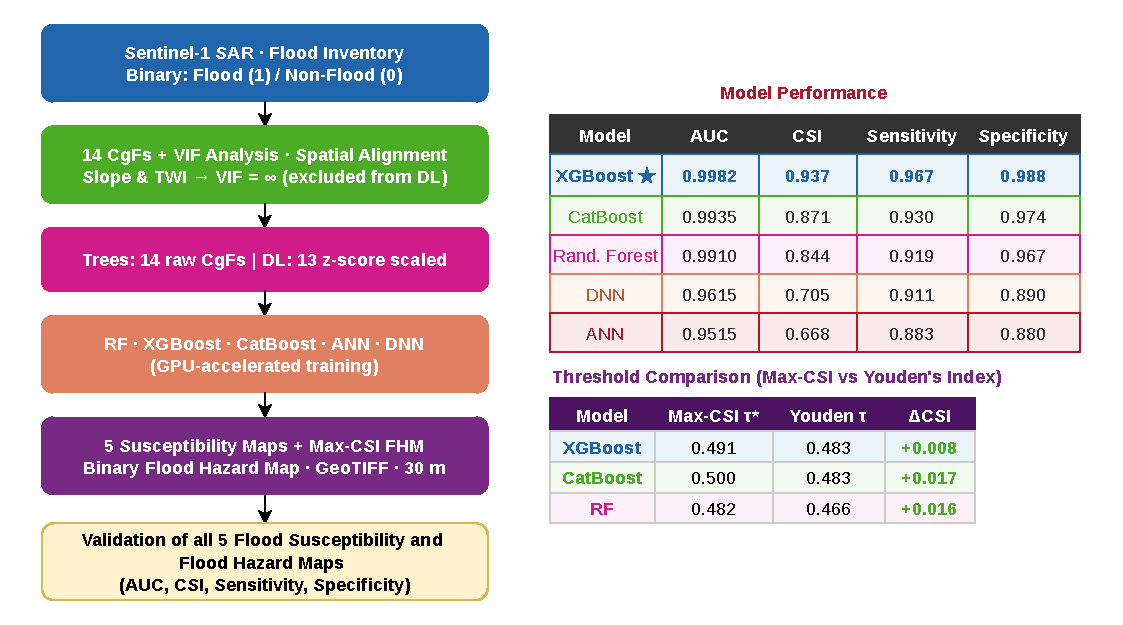
\includegraphics[width=\textwidth]{Figures/Graphical_Abstract.pdf}
    \caption*{\textbf{Graphical Abstract.} End-to-end overview of the study: data inputs (multi-mission SAR (ENVISAT ASAR + Sentinel-1) + fourteen CgFs), five-model susceptibility comparison, Max-CSI threshold optimisation, and the final XGBoost binary FHM for Khagaria district, Bihar.}
\end{figure}

\newpage

%% ============================================================
%%  1. INTRODUCTION
%% ============================================================
\section{Introduction}

Floods are the most spatially extensive and socially disruptive of all natural hazards, responsible for approximately 40\% of all disaster events globally and disproportionately affecting densely populated alluvial environments \citep{dartmouth2023, wmo2020, UNDRR2020}. During 2000--2019, floods killed over 100,000 people and affected 1.65 billion, with losses concentrated in monsoon-driven Asian river systems \citep{UNDRR2020}. In South Asia, where the Indo-Gangetic Plain concentrates hundreds of millions of people in low-lying terrain drained by glacier-fed Himalayan rivers, this exposure reaches its most acute expression. Bihar state alone sees nearly 73\% of its geographical area --- roughly 68,800 km\textsuperscript{2} --- exposed to recurrent inundation \citep{fmiscwrd2024, ray2019}, with average annual flood losses exceeding 12 billion INR over the past two decades \citep{beams2024}. The annual flood cycle is driven by the synchronised peak discharge of the Ganga and its northern tributaries --- the Kosi, Gandak, Burhi Gandak, Bagmati, and Kamla Balan --- whose origins in the geologically young and tectonically active Himalayas deliver exceptional sediment loads onto a near-flat alluvial plain \citep{gajre2017, sinha2008}. Bed aggradation, channel braiding, and frequent avulsions, compounded by engineering embankments that impede natural drainage and concentrate breach risk, render North Bihar among the most persistently flood-affected regions on Earth \citep{beams2024, mishra2018, Jha2012}. Anthropogenic climate change is further intensifying South Asian Monsoon variability and extreme precipitation frequency \citep{ipcc2021, Singh2022, Mishra2020}, making the development of accurate, high-resolution, and operationally actionable flood hazard frameworks an urgent scientific and policy priority.

Classical flood inundation modelling --- principally physics-based hydrodynamic models such as HEC-RAS, MIKE FLOOD, and LISFLOOD-FP --- offers mechanistic rigour but imposes formidable data demands: high-resolution bathymetric surveys, stream gauge networks, and extensive calibration datasets rarely available in data-scarce developing regions \citep{teng2017, neal2021, Bates2010}. These constraints have catalysed the rise of data-driven approaches leveraging satellite remote sensing and geographic information systems (GIS) to derive flood susceptibility estimates from environmental proxies. Early statistical methods --- Frequency Ratio (FR), Weights of Evidence (WoE), and Logistic Regression (LR) --- established the foundational framework of linking terrain-derived conditioning factors (CgFs) to historical flood occurrence inventories \citep{nampak2014, rahmati2016, Chapi2017}. ML successors --- Support Vector Machines \citep{hong2018}, RF \citep{tehrany2014, Pandey2021FrontEarth, Arora2021ANFIS}, and gradient-boosted tree ensembles \citep{chen2016, prokhorenkova2018} --- progressively improved predictive performance through their capacity to model non-linear predictor-response relationships. The contemporary state-of-the-art in geospatial hazard susceptibility is led by XGBoost and CatBoost, which have produced strong results across landslide \citep{Arabameri2021, Iban2022}, gully erosion \citep{zhang2022}, and flood mapping applications \citep{wang2020, li2021, Nguyen2022, Costache2022, Pourghasemi2020, Arora2025SciRep, Arora2022SERRA, Arora2024Argens}.

In parallel, the broader DL revolution has prompted increasing adoption of Artificial Neural Network (ANN) and Deep Neural Network (DNN) architectures for hydrological modelling and flood prediction, motivated by their theoretical capacity to extract hierarchical feature representations from raw input data \citep{sit2020, Hu2019, Mosavi2018, Ahmadlou2020JFRM}. DL models have achieved notable successes in time-series streamflow forecasting \citep{Kratzert2018, Shen2018}, rainfall--runoff modelling \citep{Frame2022}, and large-scale numerical weather prediction \citep{Bi2023, Lam2023, Rasp2021}, where the temporal continuity, high dimensionality, and volume of training data play directly to the strengths of recurrent and Transformer architectures. In hydrological nowcasting and medium-range weather forecasting, DL models have even begun challenging numerical weather prediction systems built over decades of physics-based development \citep{Bi2023, Lam2023}. These successes have led to a widespread but imprecise assumption that DL represents a universal improvement over classical ML in hydrology --- an assumption that does not hold when the task involves structured, low-dimensional tabular data.

Flood susceptibility mapping is fundamentally a tabular classification problem: each training sample is a pixel described by a finite row of terrain-derived attributes. In this structural setting, a body of rigorous benchmark evidence demonstrates that tree-based ensemble methods consistently outperform DL. \citet{grinsztajn2022} evaluated 45 diverse tabular datasets and found tree-based models retained a decisive advantage, attributing this to their superior inductive bias for the irregular, non-smooth, axis-aligned decision boundaries that characterise structured environmental data --- boundaries fundamentally different from the smooth manifolds that neural networks are biased towards learning. \citet{shwartzziv2022} corroborated this, arguing that DL requires dataset scales rarely attained in district-level geospatial inventories to overcome these architectural disadvantages. \citet{mcelfresh2023} extended the analysis to 176 datasets and reached the same conclusion: no DL architecture consistently dominates tree ensembles on tabular tasks. The physical rationale is transparent: flood susceptibility in alluvial terrain is governed by threshold-type rules operating in feature space --- a pixel floods if its elevation falls below a critical value AND its proximity to a river is within a threshold distance AND local drainage is impeded. These axis-aligned conditions are precisely what recursive binary partitioning in decision trees is designed to represent \citep{breiman2001, Popov2021}. Neural networks, applying stacked linear transformations with smooth activations, impose a prior favouring smooth decision surfaces --- a prior structurally mismatched to the step-wise physical logic of alluvial flood inundation. Furthermore, DL models applied to small or medium geospatial inventories are prone to producing poorly calibrated probability outputs even when AUC is competitive \citep{Niculescu-Mizil2005, zadrozny2002} --- the pattern precisely observed in the DNN and ANN results of this study, where competitive AUC coexists with markedly inferior CSI and anomalously low optimal thresholds.

A related and underexplored methodological gap in the flood mapping literature concerns the transition from continuous susceptibility probability maps to operationally deployable binary flood hazard maps (FHMs). Most studies apply a fixed 0.5 probability cut-off or Youden's Index \citep{youden1950} without accounting for the asymmetric error costs of flood detection, where missed flood zones (false negatives) carry far greater societal consequences --- in terms of loss of life, displacement, and infrastructure damage --- than unnecessary hazard designations (false positives). The Critical Success Index (CSI) --- also known as the Threat Score, originally formalised for severe weather warning verification \citep{schaefer1990} --- simultaneously penalises all three error types (TP, FP, FN) and does not reward true negatives, making it uniquely suited to operational flood mapping in environments where the non-flood class dominates by area \citep{mason2003, Pham2021, nguyen2021}. Despite this suitability, comparative evaluations of threshold optimisation methods for flood hazard zonation remain scarce. The present study operationalises Max-CSI as the primary thresholding criterion and benchmarks it rigorously against Youden's Index across all five models.

The flood inventory underpinning this study was constructed by integrating multi-year SAR-derived flood extents from the 2008, 2020, and 2021 monsoon events in Khagaria district --- an approach that captures the multi-event flood envelope rather than a single-season snapshot, following the multi-temporal inventory framework validated for the Lower Kosi River Basin \citep{Arora2022SERRA}. Sentinel-1 Synthetic Aperture Radar (SAR) imagery in C-band, available through the Copernicus Programme, enables reliable water surface detection through cloud cover and rain-band obscuration during peak monsoon inundation \citep{Twele2016, DeVries2020, dasgupta2018} --- conditions that render optical sensors operationally non-functional.

This study addresses these interconnected gaps through a systematic multi-model comparative analysis of flood susceptibility mapping and FHM derivation in Khagaria district, Bihar --- a district that, despite its extraordinary and well-documented flood exposure at the convergence of seven major river systems, has not been the subject of a rigorous pixel-level ML susceptibility study integrating both tree-based ensembles and DL architectures with a principled threshold optimisation framework. Specifically, the study: (i) constructs a fourteen-CgF geospatial database integrating a multi-year Sentinel-1 SAR-derived flood inventory with terrain, land cover, hydrological, and geological predictors; (ii) implements VIF-based collinearity screening to ensure appropriate feature selection for each model class; (iii) trains and validates RF, XGBoost, CatBoost, ANN, and DNN under a unified Hybrid Prediction Pipeline; (iv) applies SHapley Additive exPlanations (SHAP) to quantify conditioning factor importance across all five models;  (v) derives binary FHMs using Max-CSI threshold optimisation and compares performance against Youden's Index; and (vi) produces pixel-level flood hazard zonation at 30 m resolution to support the DDMA of Khagaria in operational preparedness and mitigation planning.

%% ============================================================
%%  2. STUDY AREA
%% ============================================================
\section{Study Area}

\subsection{Geographical Setting and Topography}

Khagaria district is situated in the heart of North Bihar, spanning latitudes 25\textdegree15'N to 25\textdegree44'N and longitudes 86\textdegree17'E to 86\textdegree52'E (Figure~\ref{fig:study_area}). The district encompasses approximately 1,486 km\textsuperscript{2} and is administratively part of the Munger Division, bounded by Saharsa and Madhepura to the north, Bhagalpur and Munger to the south, Begusarai and Samastipur to the west, and Katihar to the east \citep{khagdist2024}. The topography is quintessential of the Gangetic deltaic plains --- flat, low-lying, and devoid of significant relief. District elevations span approximately 36 m to 47 m above mean sea level, declining gently from north-northwest towards south-southeast --- a characteristic gradient of the Gangetic alluvial plain that severely limits natural drainage capacity \citep{khagdist2024}. This subdued topography constrains drainage efficiency and facilitates stagnation and prolonged recession of floodwaters. Soils are predominantly fine-textured alluvial deposits --- silty clay loams and silty loams --- with low infiltration capacity, exacerbating surface runoff and inundation \citep{NBSSLUPbihar2020}.

\subsection{The District of Seven Rivers}

Khagaria's hydrological identity is defined by its status as the convergence zone for seven major river systems, justifying its epithet as the ``drainage sink of North Bihar'':

\begin{itemize}
    \item \textbf{The Ganga:} The master drain, forming the district's southern boundary. Its elevated stage during monsoon peak acts as a hydraulic barrier, impeding tributary discharge and generating severe drainage congestion --- locally termed \textit{paani band} \citep{beams2024}.
    \item \textbf{The Kosi (Saptakoshi):} Known historically as the ``Sorrow of Bihar,'' the Kosi is notorious for exceptionally high bedload sediment flux and geologically recent mega-avulsions, having shifted approximately 120 km westward over roughly two-and-a-half centuries through repeated avulsion cycles \citep{sinha2008, mishra2018}. The Kosi carries approximately 100--150 million tonnes of sediment annually, progressively raising its bed above the surrounding floodplain and increasing avulsion risk \citep{sinha2008}.
    \item \textbf{The Burhi Gandak:} A meandering river joining the Ganga near Gogri Jamalpur; embankment breaches are a recurrent cause of inundation, particularly in Gogri and Mansi blocks.
    \item \textbf{The Bagmati and Kamla Balan:} Himalayan tributaries with flashy regimes, high suspended sediment loads, and documented susceptibility to embankment breaching during sustained high-discharge episodes \citep{mishra2018}.
    \item \textbf{The Kareh and Kali Kosi:} Significant distributary channels contributing to peripheral block inundation in Alauli, Beldaur, and Parbatta blocks.
\end{itemize}

The convergence of these systems within a single low-lying district means that multiple rivers may peak simultaneously, preventing drainage of any individual channel and producing multi-week inundation episodes. The \textit{chaur} depressions --- oxbow-lake remnants and shallow inter-levee basins scattered throughout the district --- act as secondary water retention zones and experience the most prolonged flooding.

\subsection{Climate and Flood History}

Khagaria experiences a humid subtropical climate (K\"{o}ppen: Cwa). The Southwest Monsoon (June--September) delivers approximately 1,255 mm annually with high inter-annual variability \citep{beams2024}. Historically significant events include the 1987 Kosi dam-burst (damages exceeding 68 billion INR), the 2004 Bagmati-Kamla flood, the catastrophic 2008 Kosi course-change near Kusaha, Nepal --- which shifted the river approximately 120 km eastward in days and inundated over 3,400 km\textsuperscript{2} of Bihar \citep{bhuvan2010, mishra2018} --- and the 2024 double-peak inundation associated with cyclonic-monsoon interactions \citep{tatatrusts2024}. The 2020 and 2021 floods, which form part of the inventory used in this study, inundated 839.40 km\textsuperscript{2} of Khagaria as delineated from Sentinel-1 SAR imagery (Figure~\ref{fig:study_area}).

\begin{figure}[H]
    \centering
    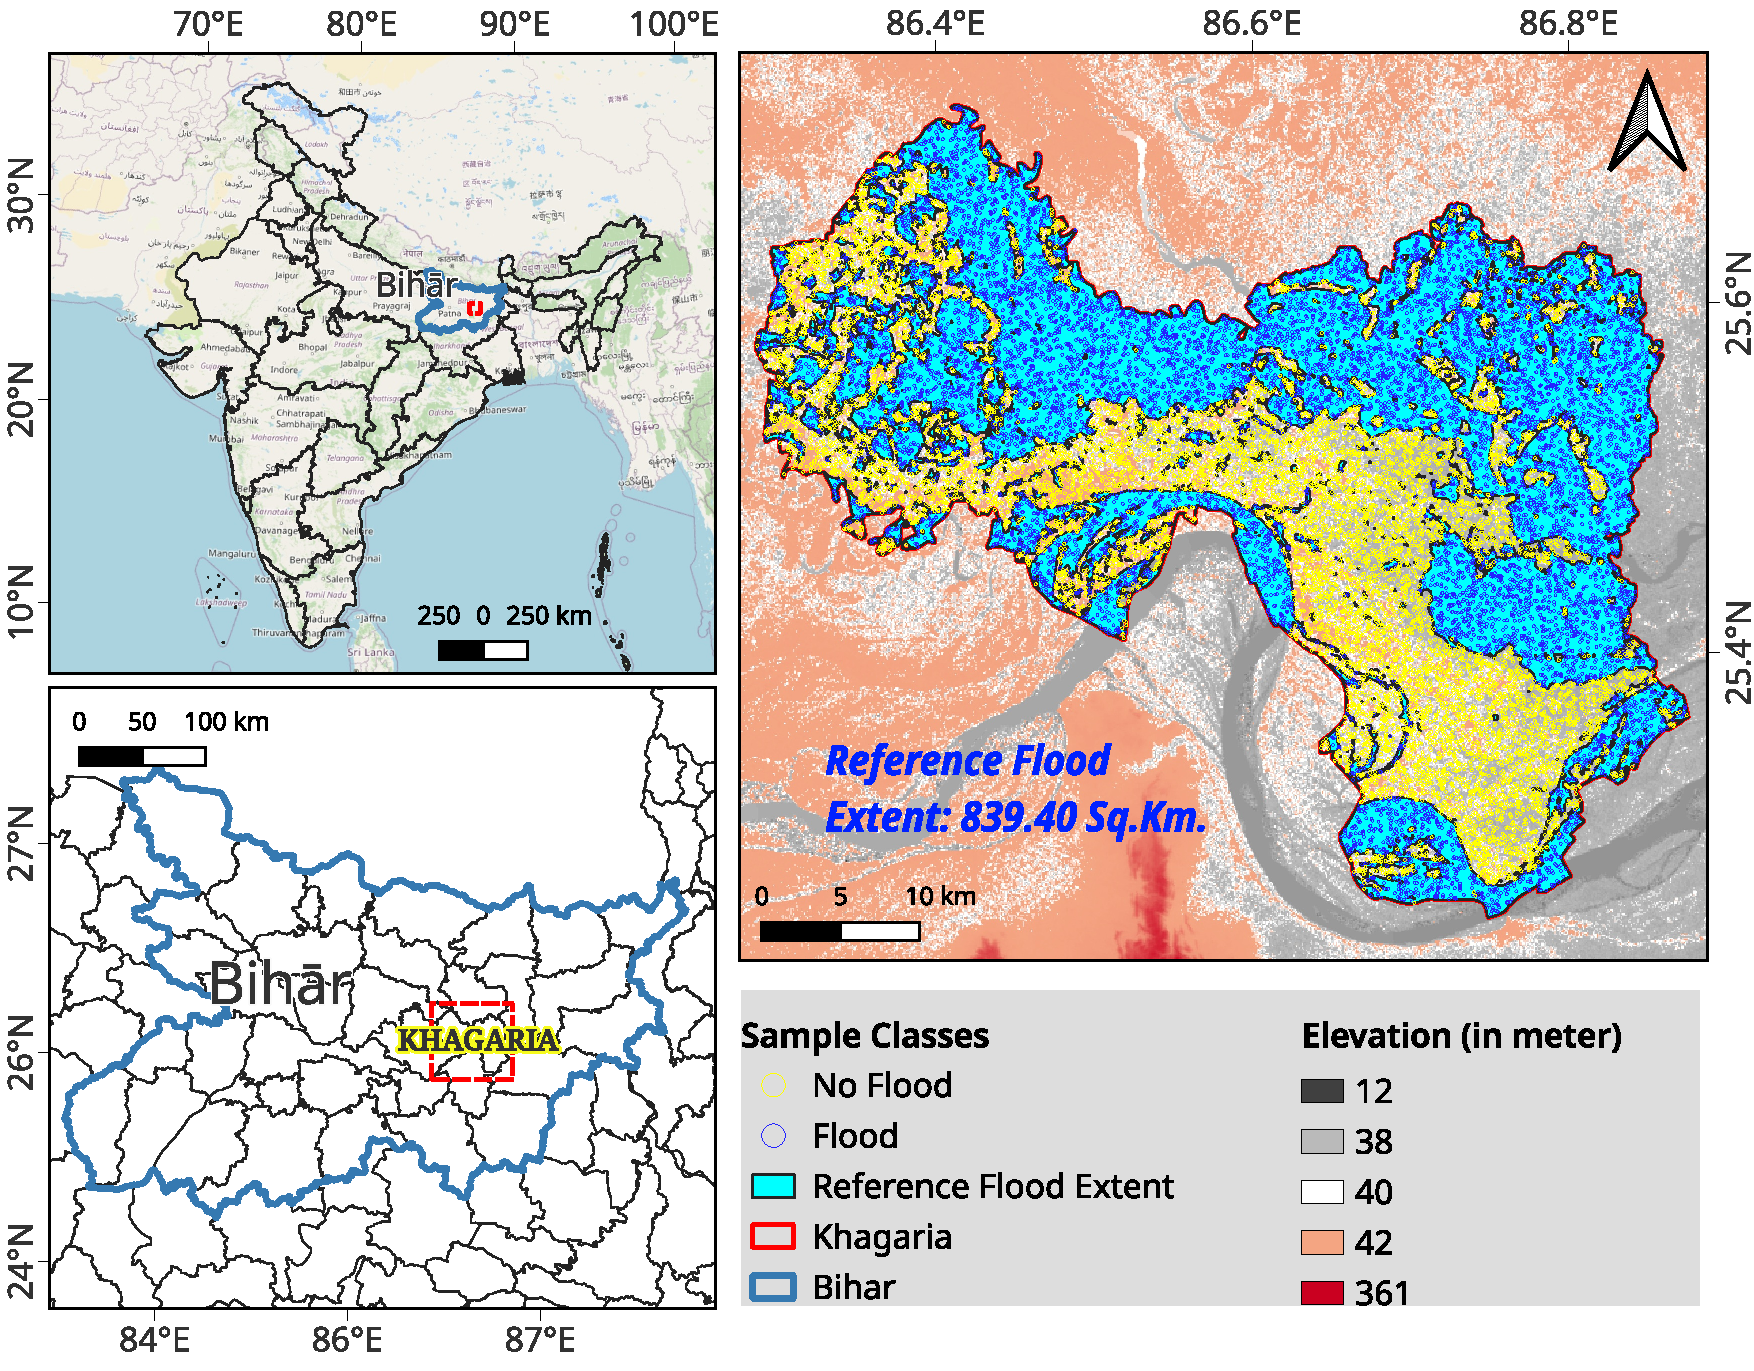
\includegraphics[width=\textwidth]{Figures/Location_map.pdf}
    \caption{Study area: Khagaria district, North Bihar, India. (Left panels) Bihar within India and Khagaria within Bihar; (Right) district boundary with block boundaries, seven major river systems, and the spatial distribution of the multi-year Sentinel-1 SAR-derived flood and non-flood inventory samples overlaid on an elevation-based background. The reference flood extent (839.40 km\textsuperscript{2}) is shown in cyan. The district occupies the hydrological sink of North Bihar, receiving simultaneous peak discharge from the Kosi, Bagmati, Burhi Gandak, and other tributaries before their confluence with the Ganga.}
    \label{fig:study_area}
\end{figure}

%% ============================================================
%%  3. MATERIALS AND METHODS
%% ============================================================
\section{Materials and Methods}

The methodological workflow comprises six sequential phases: (1) flood inventory construction from multi-year Sentinel-1 SAR, (2) CgF preparation and spatial alignment, (3) multi-collinearity analysis via VIF, (4) model training under the Hybrid Prediction Pipeline, (5) spatial susceptibility prediction, and (6) threshold-optimised FHM derivation (Figure~\ref{fig:workflow}).

\begin{figure}[H]
    \centering
    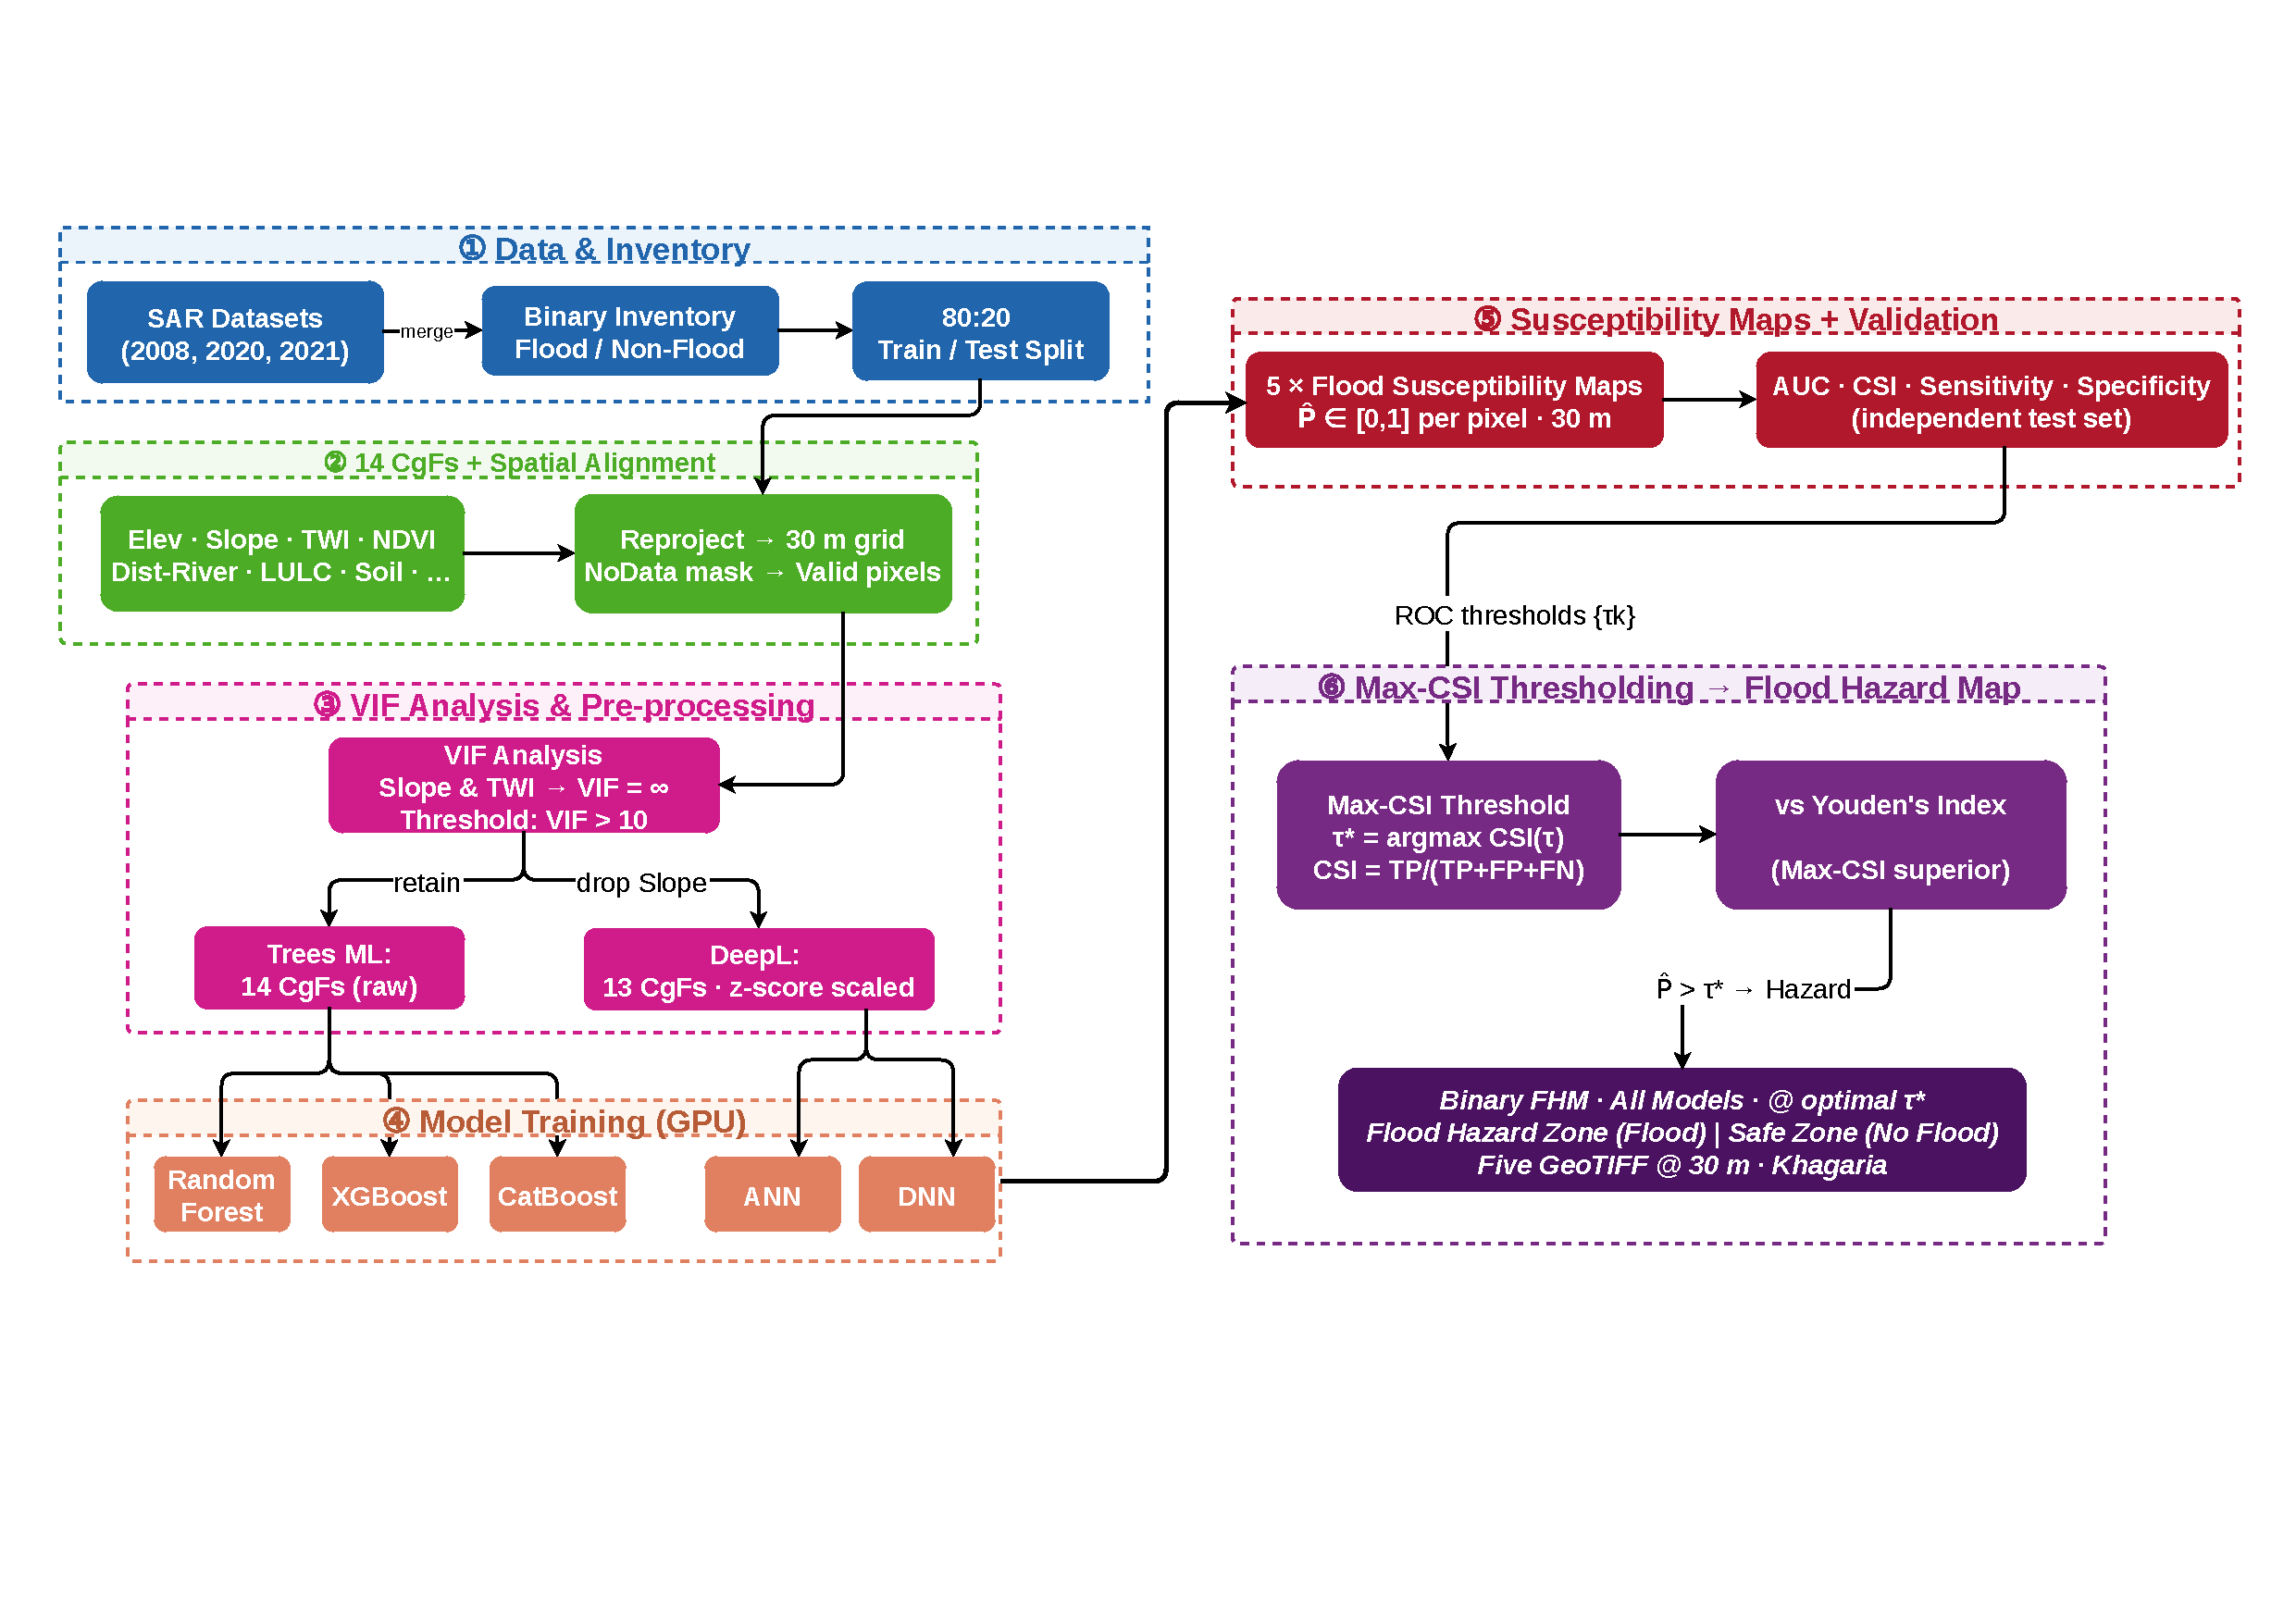
\includegraphics[width=\textwidth]{Figures/FHM_Khagaria_Methodology_Flowchart.pdf}
    \caption{Methodological workflow of the Hybrid Prediction Pipeline. The pipeline applies separate feature preprocessing for tree-based and DL model branches, followed by unified Max-CSI threshold optimisation to derive final binary FHMs.}
    \label{fig:workflow}
\end{figure}

\subsection{Flood Inventory: Ground Truth Construction}

The dependent variable is a binary flood inventory raster classifying each pixel as Flood (1) or Non-Flood (0). The inventory was constructed by integrating SAR-derived flood extents from three major flood events in Khagaria: the 2008 Kosi avulsion flood, and the 2020 and 2021 monsoon peak inundation episodes. This multi-year integration approach captures the full spatial envelope of flood occurrence rather than a single-event snapshot, following the methodology validated for the Lower Kosi River Basin \citep{Arora2022SERRA}. The resulting reference flood extent covers 839.40 km\textsuperscript{2} of Khagaria district.

SAR imagery from two sensor missions was acquired during peak flood episodes to build the multi-temporal inventory. For the 2008 Kosi avulsion event, ENVISAT ASAR Wide Swath Mode (WSM) scenes were used, providing C-band backscatter at approximately 150 m native resolution resampled to 30 m \citep{Twele2016}; the 2008 dataset constitutes the most important inventory event given the exceptional spatial extent of that avulsion. For the 2020 and 2021 monsoon peak inundations, Sentinel-1A/B Ground Range Detected (GRD) IW-mode imagery (C-band, 5.405 GHz; VV polarisation; 10 m native, resampled to 30 m) was used \citep{DeVries2020, dasgupta2018}. SAR imagery was preferred over optical sensors for its capability to penetrate persistent cloud cover and monsoon rain-band obscuration that renders optical data non-functional during peak inundation \citep{srivastava2017}. Open water exhibits distinctly lower backscatter than vegetated or built-up surfaces due to specular reflection, enabling reliable water/non-water discrimination via threshold-based change-detection \citep{bauer2015, Twele2016}. To construct the composite flood envelope, single-event binary flood masks were produced independently for each year and then merged by spatial union at the 30 m grid. Pixels flooded in any of the three events were retained as flooded (spatial union), ensuring the inventory represents the maximum observed inundation extent rather than any single event, following the multi-temporal protocol validated for the Lower Kosi River Basin \citep{Arora2022SERRA}. Non-flood reference pixels were sampled from areas demonstrably unaffected throughout the entire inventory period at approximately 1:1 flood-to-non-flood ratio to prevent severe class imbalance. The inventory was partitioned 80:20 (training:testing) using stratified random sampling:
\begin{equation}
    \text{Training set} = 80\%\ \text{of valid pixels},\quad \text{Test set} = 20\%\ \text{of valid pixels}
\end{equation}

\subsection{Flood Conditioning Factors}

Fourteen CgFs were selected based on a systematic literature review of flood susceptibility modelling \citep{khosravi2018, tehrany2019, rahmati2016, Costache2022, Pourghasemi2020, Pandey2021FrontEarth, Arora2022SERRA} and the physico-geographic characteristics of Khagaria's alluvial environment (Table~\ref{tab:factors}). The selection spans five thematic domains: topographic controls (Elevation, Slope, Curvature, Aspect, TWI, SPI), hydrological proximity (Distance to River, Stream Density), land surface characteristics (LULC, Geomorphology, Soil), geological substrate (Lithology), climatic forcing (Rainfall), and anthropogenic drainage modification (Distance to Roads). All CgFs were prepared as GeoTIFF rasters aligned to a common reference grid at 30 m spatial resolution.

\begin{table}[H]
\centering
\caption{Flood conditioning factors (CgFs) employed in this study.}
\label{tab:factors}
\small
\begin{tabularx}{\linewidth}{@{} c l l X @{}}
\toprule
\textbf{No.} & \textbf{Factor} & \textbf{Source} & \textbf{Hydrological Rationale} \\
\midrule
1  & Aspect              & Derived (SRTM)            & Directional exposure influences moisture and evapotranspiration \\
2  & Curvature           & Derived (SRTM)            & Identifies concave surfaces as water collection zones \\
3  & Distance to River   & Derived (SRTM)            & Proximity increases exposure to bank overflow \\
4  & Distance to Roads   & OSM                       & Road embankments alter local drainage patterns \\
5  & Elevation           & SRTM 30 m                 & Primary control on inundation depth and extent \\
6  & Geomorphology       & GSI                       & Floodplain geomorphological unit classification \\
7  & Lithology           & GSI                       & Bedrock type influences groundwater dynamics and permeability \\
8  & LULC                & Sentinel-2                & Vegetation and impervious cover modulate infiltration \\
9  & Rainfall            & IMD Gridded (1901-2021)   & Primary triggering factor for surface runoff generation \\
10 & Slope               & Derived (SRTM)            & Controls overland flow velocity; near-zero slopes intensify ponding \\
11 & Soil                & HWSD, FAO                 & Controls infiltration rate and hydraulic conductivity \\
12 & Stream Density      & Derived (SRTM)            & Dense networks accelerate runoff concentration \\
13 & Stream Power Index  & Derived (SRTM)            & Measures erosive power of overland flow \\
14 & TWI                 & Derived (SRTM)            & Quantifies soil saturation propensity and flow accumulation \\
\bottomrule
\end{tabularx}
\end{table}

\subsection{Data Preprocessing and Spatial Alignment}

All CgF rasters were reprojected to the reference coordinate reference system (UTM Zone 45N, WGS84) and resampled using nearest-neighbour interpolation via \texttt{rasterio.warp.reproject()} \citep{gillies2019} to ensure an identical grid geometry across all layers. A binary valid mask was computed:
\begin{equation}
    \text{mask}_{i} = \bigcap_{k=1}^{K}\Big[\big(\text{value}_{k,i} \neq -9999\big) \cap \big(\neg\,\text{NaN}_{k,i}\big)\Big]
\end{equation}
where $i$ indexes pixels and $k$ indexes layers, excluding all pixels with missing values in any CgF or the flood inventory. Neural network architectures additionally require normalised inputs for stable gradient descent convergence \citep{lecun2012, Goodfellow2016}; all features were scaled using zero-mean, unit-variance standardisation:
\begin{equation}
    x' = \frac{x - \mu}{\sigma}
\end{equation}
where $\mu$ and $\sigma$ are training-set statistics applied consistently to the test set and full spatial prediction rasters to prevent data leakage. Tree-based models were trained on raw (unscaled) values, as they are invariant to monotonic transformations \citep{breiman2001}.

\subsection{Multi-Collinearity Analysis: Variance Inflation Factor}

Multi-collinearity among predictor variables can destabilise neural network gradient descent and inflate prediction variance \citep{dormann2013, Belsley2005}. The VIF was computed for each CgF:
\begin{equation}
    \text{VIF}_{j} = \frac{1}{1 - R^{2}_{j}}
\end{equation}
where $R^{2}_{j}$ is the coefficient of determination from regressing the $j^{\text{th}}$ predictor on all remaining predictors. A VIF threshold of 10 was adopted \citep{dormann2013, OBrien2007}. Both Slope and TWI exhibited effectively infinite VIF ($\text{VIF} \to \infty$), attributable to their algebraic interdependence:
\begin{equation}
    \text{TWI} = \ln\left(\frac{A_s}{\tan \beta}\right)
\end{equation}
where $A_s$ is the specific catchment area and $\beta$ is local slope angle. In the near-flat terrain of Khagaria (mean slope $< 0.5\textdegree$), slope values approach zero, causing $\tan \beta$ to produce extreme TWI values and a computationally singular collinearity. Both were excluded from ANN and DNN feature sets; tree-based models retained all fourteen CgFs due to their inherent robustness to collinearity through greedy split-selection. The feature correlation matrix is presented in Figure~\ref{fig:corrmatrix} and full VIF scores in Table~\ref{tab:vif}. The VIF analysis was conducted on a stratified subsample of 50,000 valid pixels for computational tractability.

\begin{figure}[H]
    \centering
    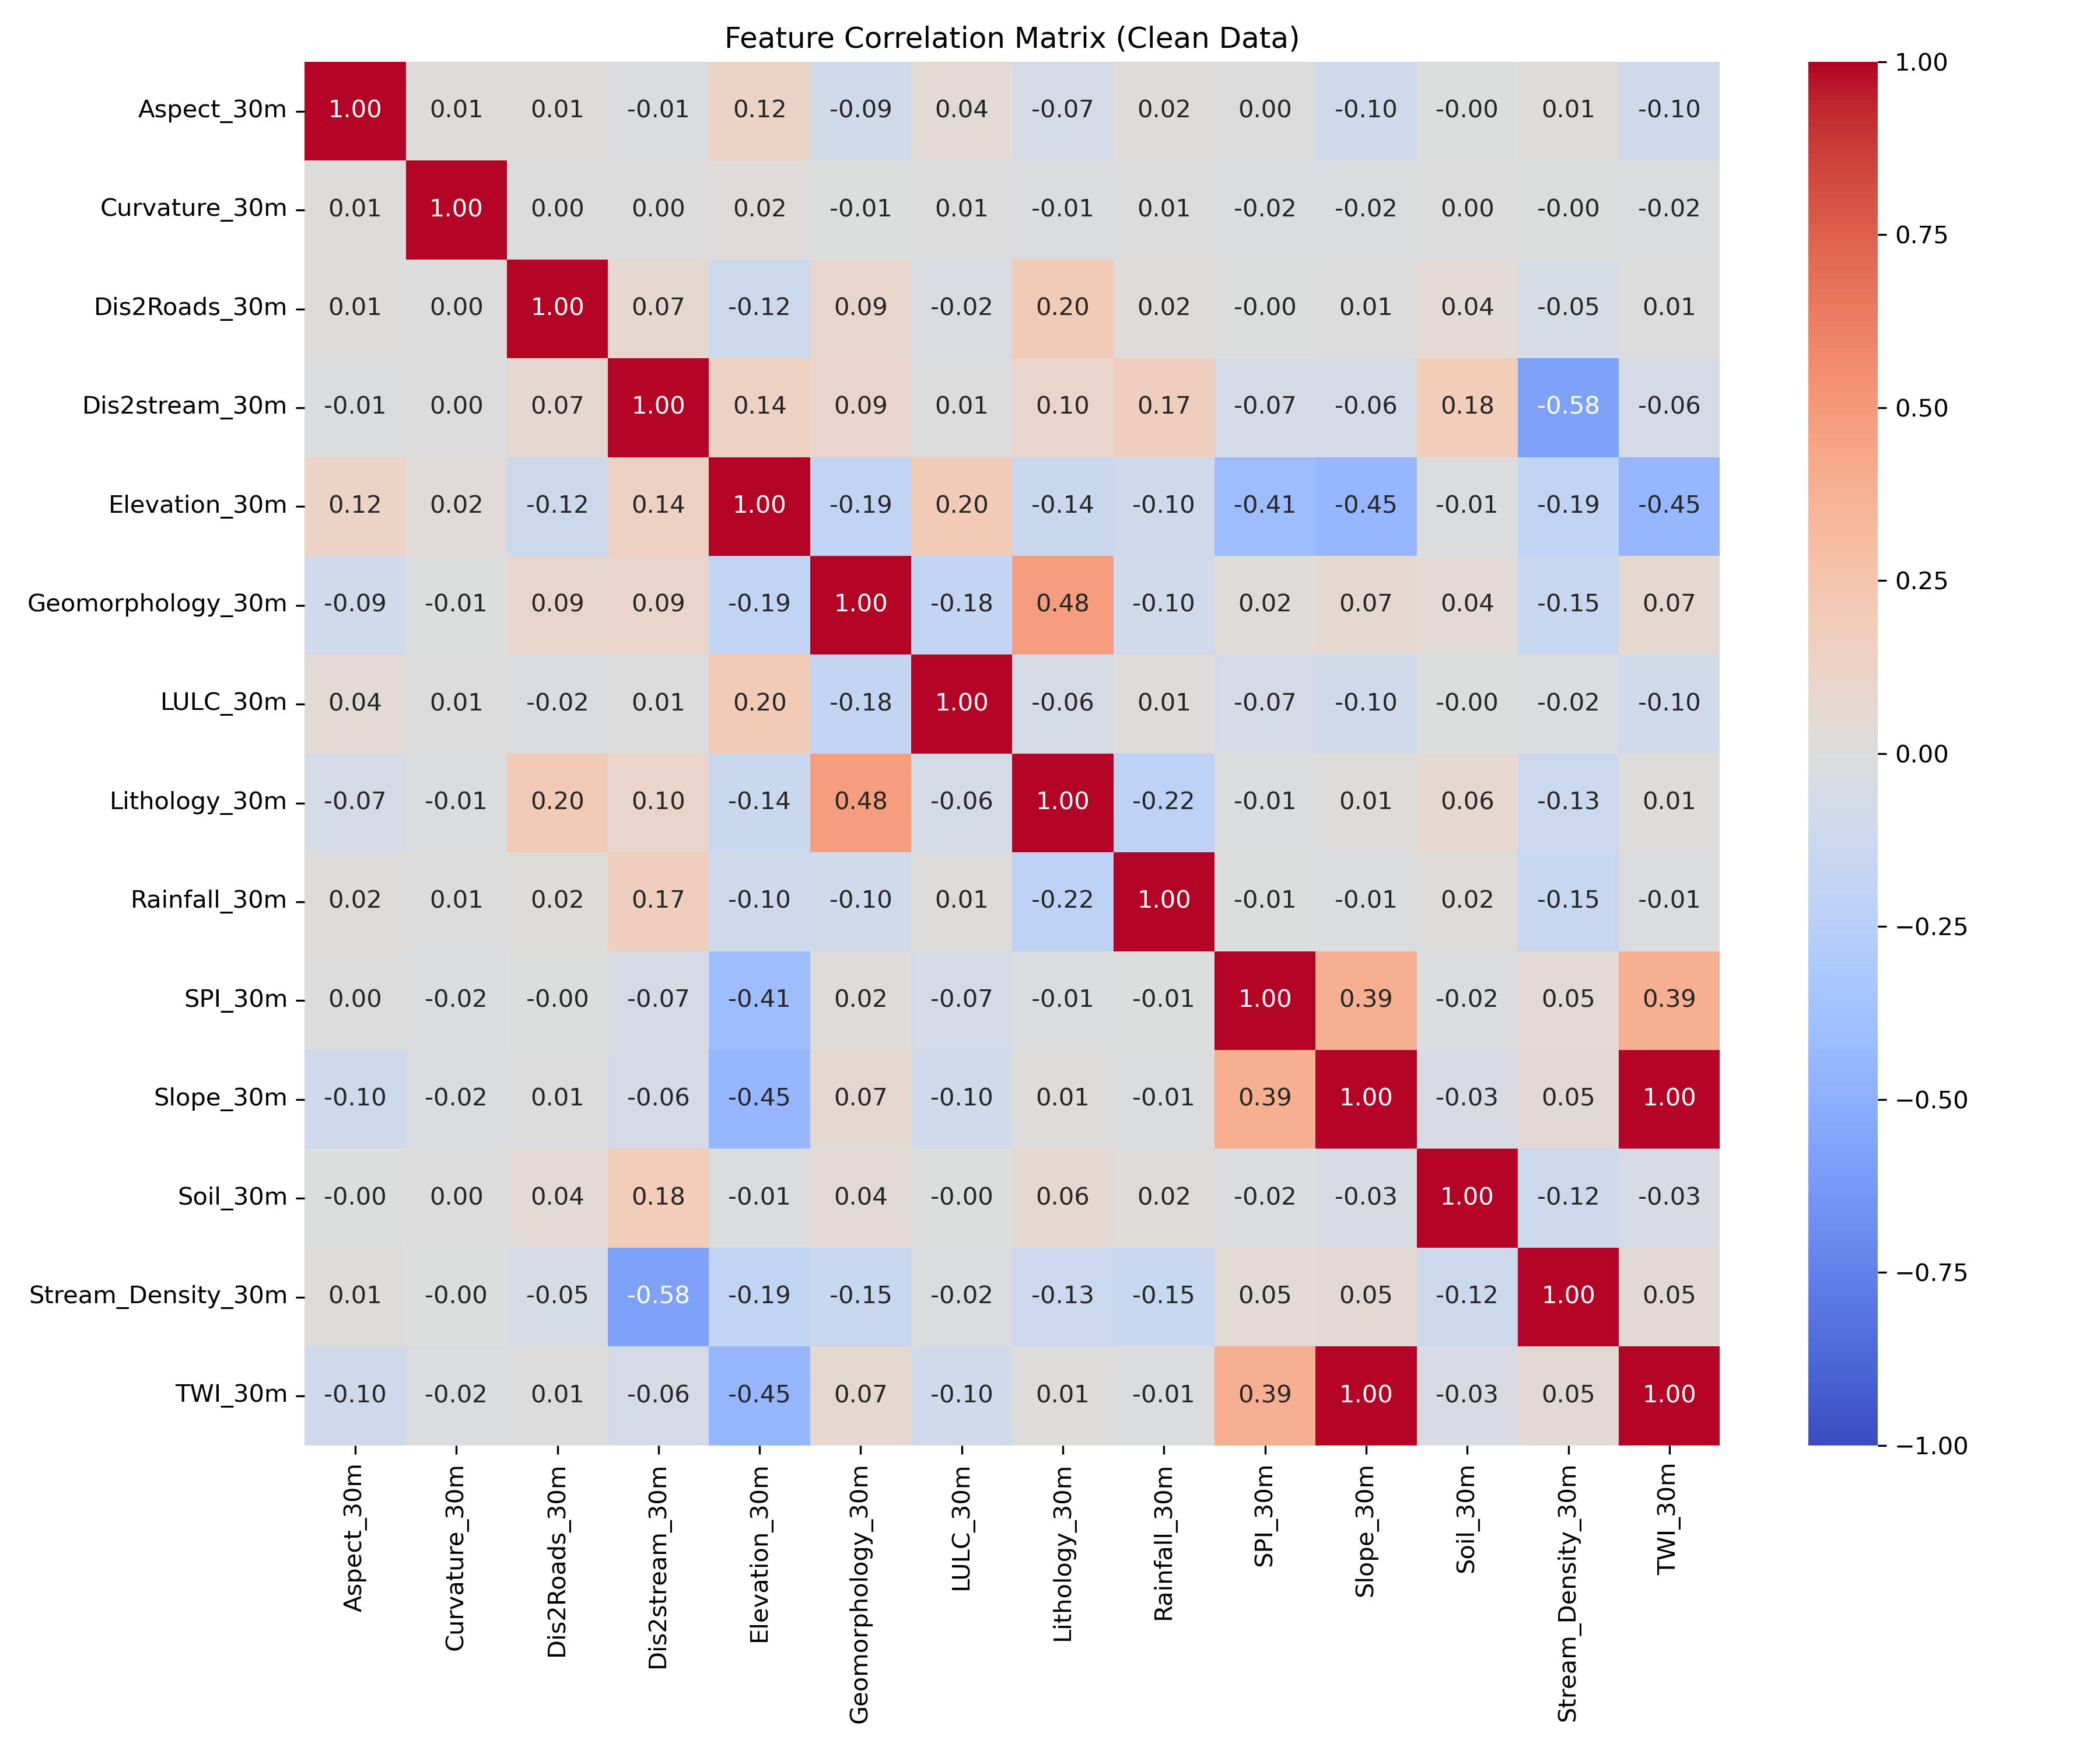
\includegraphics[width=0.95\textwidth]{Figures/Correlation_Matrix_Robust.png}
    \caption{Pearson correlation matrix for the fourteen CgFs computed from a 50,000-pixel subsample. The perfect correlation ($r = 1.00$) between Slope\textsubscript{30m} and TWI\textsubscript{30m} confirms their algebraic interdependence under the TWI formulation, consistent with the infinite VIF values obtained for both in the near-zero-slope alluvial terrain of Khagaria. A moderate negative correlation ($r = -0.58$) between Distance to Stream and Stream Density reflects the geomorphological relationship between channel proximity and drainage network density in the Gangetic floodplain. A moderate negative correlation between Elevation and TWI ($r = -0.45$) and Elevation and SPI ($r = -0.41$) is expected, as lower elevations accumulate more flow. All other inter-factor correlations are below $|r| = 0.5$, confirming the adequacy of the remaining twelve features for neural network training.}
    \label{fig:corrmatrix}
\end{figure}

\subsection{Model Architectures and Training}

\subsubsection{Random Forest}
RF is a bagging ensemble constructing $T$ independent decision trees, each trained on a bootstrap resample using a random subset of $\sqrt{p}$ features at each split node \citep{breiman2001, belgiu2016}. Predictions are averaged probability estimates across all trees. A GPU-accelerated cuML implementation was employed with $T = 150$ trees and maximum depth of 16, using all 14 raw CgFs without scaling.

\subsubsection{XGBoost}
XGBoost \citep{chen2016} constructs an additive ensemble of decision trees sequentially, each fitted to the negative gradient of a regularised second-order Taylor expansion of the loss:
\begin{equation}
    \mathcal{L}^{(t)} \approx \sum_{i=1}^{n} \left[g_i f_t(x_i) + \frac{1}{2}h_i f_t^2(x_i)\right] + \Omega(f_t)
\end{equation}
where $g_i$ and $h_i$ are the first and second derivatives of the loss, and $\Omega(f_t)$ penalises tree complexity via $L_1$ and $L_2$ regularisation. Hyperparameters: maximum depth = 8, learning rate = 0.1, subsample = 0.8, up to 1,000 boosting rounds with early stopping (20 rounds without AUC improvement). GPU histogram acceleration (\texttt{tree\_method=hist}, \texttt{device=cuda}) was used.

\subsubsection{CatBoost}
CatBoost \citep{prokhorenkova2018} introduces two algorithmic innovations: (i) \textit{Ordered Boosting}, using a random permutation to compute unbiased gradient estimates and mitigate target leakage; and (ii) \textit{Oblivious Trees} (symmetric decision trees), applying the same split at all nodes of a given depth level for efficient and regularised inference \citep{Dorogush2018}. Training: 800 iterations, learning rate 0.1, depth 8, GPU acceleration.

\subsubsection{Artificial Neural Network}
The ANN employed a shallow feed-forward topology trained on 12 VIF-filtered, standardised CgFs:
\begin{multline}
    \text{Input}(p) \to \text{Linear}(64) \to \text{ReLU} \to \text{BatchNorm} \to \text{Dropout}(0.3) \\
    \to \text{Linear}(32) \to \text{ReLU} \to \text{Linear}(1) \to \sigma
\end{multline}
where $\sigma$ is the sigmoid activation and $p = 12$ (excluding Slope and TWI). Batch normalisation and dropout serve as regularisation against overfitting \citep{ioffe2015, srivastava2014}. Loss: Binary Cross-Entropy with Logits; optimisation: Adam \citep{kingma2014}, learning rate $10^{-3}$, 15 epochs, batch size 4,096. Implemented in PyTorch \citep{paszke2019} with CUDA acceleration.

\subsubsection{Deep Neural Network}
The DNN extended the ANN by increasing depth:
\begin{multline}
    \text{Input}(p) \to \text{Linear}(128) \to \text{ReLU} \to \text{BN} \to \text{Drop}(0.4) \to \text{Linear}(64) \\
    \to \text{ReLU} \to \text{BN} \to \text{Drop}(0.3) \to \text{Linear}(32) \to \text{ReLU} \to \text{Linear}(1) \to \sigma
\end{multline}
The deeper architecture theoretically enables hierarchical feature abstraction but, as the results demonstrate, confers no performance advantage over tree ensembles for this tabular dataset \citep{grinsztajn2022, shwartzziv2022}. The same training configuration as the ANN was applied: Adam, $\text{lr} = 10^{-3}$, 15 epochs, batch size 4,096.

\subsection{SHAP Explainability Analysis}
\label{sec:shap_method}

To provide model-conditioned, physically interpretable importance scores, SHAP \citep{lundberg2017, lundberg2020} were computed post-training for all five models. SHAP uniquely satisfies the four Shapley axioms --- efficiency, symmetry, linearity, and dummy \citep{shapley1953} --- guaranteeing a fair attribution of each prediction to each input feature that is both theoretically sound and locally accurate.

\subsubsection{GPU Acceleration per Model Type}

\begin{description}[style=nextline, align=left]
  \item[\textbf{XGBoost:}] Exact GPU TreeSHAP via \texttt{booster.predict(pred\_contribs=True)} on \texttt{device=cuda}.  This is XGBoost's native SHAP path, returning the full Shapley attribution matrix in a single GPU call with no external SHAP wrapper required. Output: $(N,\,p+1)$ float32 array; last column is the bias term and is discarded.

  \item[\textbf{CatBoost:}] GPU SHAP via \texttt{model.get\_feature\_importance(data=pool, type=`ShapValues', shap\_calc\_type=`Regular')}. This routes through CatBoost's internal GPU inference engine when the model was trained with \texttt{task\_type=`GPU'}, yielding exact Shapley values aligned with the Ordered Boosting formulation.

  \item[\textbf{RandomForest:}] \texttt{shap.TreeExplainer} applied to a proxy \texttt{sklearn} RF (100 estimators, same hyperparameters) fitted on the same balanced SHAP sample, using exact C++ tree traversal.

  \item[\textbf{ANN and DNN:}] \texttt{shap.GradientExplainer} with CUDA tensors, applying Integrated Gradients \citep{Sundararajan2017} through the network in a single batched GPU pass.  This is 100--500$\times$ faster than KernelExplainer for neural architectures. Background: 200 pixels; inference batch size: 256.
\end{description}

SHAP values were computed on a balanced stratified sample of $N = 5{,}000$ pixels ($2{,}500$ flood; $2{,}500$ non-flood) drawn from the full valid-pixel domain.  Mean absolute SHAP values $\bar{|\phi_j|}$ summarise each feature's average predictive contribution in log-odds units.  For inter-model comparison, values were min--max normalised to $[0,1]$.

\subsection{Spatial Prediction}

Each trained model generated a continuous probability map $\hat{P} \in [0,1]$ for every valid pixel in Khagaria, constituting the flood susceptibility map (FSM). Neural network inference was performed in batches of 50,000 pixels to manage GPU memory. All outputs were saved as GeoTIFF files with LZW compression and float32 precision, retaining original coordinate reference system and transform metadata. For spatial visualisation, the continuous FSMs were reclassified into five susceptibility classes using Natural Breaks (Jenks) optimisation: Very Low (0.00--0.10), Low (0.10--0.33), Moderate (0.33--0.61), High (0.61--0.88), and Very High (0.88--1.00).

\subsection{Threshold Optimisation: Maximum Critical Success Index}

Converting continuous FSM probabilities to binary FHMs requires selection of a decision threshold $\tau$. Standard approaches use $\tau = 0.5$ or Youden's Index \citep{youden1950}:
\begin{equation}
    J = \text{Sensitivity} + \text{Specificity} - 1 = \text{TPR} - \text{FPR}
\end{equation}
These are suboptimal for imbalanced flood inventories where false negatives carry asymmetric operational costs. This study adopted Max-CSI \citep{schaefer1990, wilks2019}:
\begin{equation}
    \text{CSI} = \frac{\text{TP}}{\text{TP} + \text{FP} + \text{FN}}
\end{equation}
where TP, FP, and FN denote true positives, false positives, and false negatives. The CSI simultaneously penalises all three error types and does not reward true negatives (safe pixels correctly classified as safe), making it uniquely aligned with the operational objective of flood hazard detection \citep{mason2003, Pham2021}. Given ROC-curve-derived thresholds $\{\tau_k\}$ with corresponding true positive rate (TPR) and false positive rate (FPR), the CSI was computed efficiently via:
\begin{equation}
    \text{CSI}_k = \frac{\text{TPR}_k \cdot P}{P + \text{FPR}_k \cdot N}
\end{equation}
where $P$ and $N$ are the total flood and non-flood pixel counts respectively. The optimal threshold is $\tau^* = \tau_{\arg\max_k \text{CSI}_k}$. Pixels with $\hat{P} > \tau^*$ were classified as Flood Hazard Zone (1); otherwise as Safe Zone (0). A visualisation of the resulting CSI and Youden's J curves across all threshold values, alongside the achieved CSI scores at each optimal point, is presented in the Results section (Figure~\ref{fig:maxcsi}).

\subsection{Validation Metrics}

Model performance was assessed using: (1) AUC --- discrimination ability across all possible thresholds; (2) CSI at $\tau^*$ --- threshold-specific flood detection accuracy penalising TP, FP, and FN; (3) Sensitivity (TPR) --- fraction of actual flood pixels correctly identified; (4) Specificity (TNR) --- fraction of safe pixels correctly identified; and (5) overall Accuracy. These metrics jointly address both ranking ability (AUC) and operational classification performance \citep{Fawcett2006, Powers2011}. To assess generalisation, both training-set and test-set AUC are reported, and the difference quantifies overfitting tendency.

\subsection*{Use of AI Tools}
\textit{[Author note: complete this statement accurately before submission. Springer requires disclosure of generative-AI use in the Methods section where it involved editorial work beyond copy-editing --- e.g., drafting text, structuring arguments, or assisting with analysis framing. AI-assisted copy-editing for grammar, spelling, and tone does not require disclosure. Suggested wording, to be verified and adjusted: ``An AI language model (Claude, Anthropic) was used to assist with manuscript drafting, structuring, and language editing during preparation of this work. All AI-assisted content was reviewed, verified, and edited by the authors, who take full responsibility for the accuracy and integrity of the final manuscript. The AI tool was not used for data analysis, model development, or generation of results.'']}

%% ============================================================
%%  4. RESULTS
%% ============================================================
\section{Results}

\subsection{Multi-Collinearity Analysis}

The VIF analysis confirmed the anticipated collinearity structure (Table~\ref{tab:vif}). Slope and TWI both exhibited infinite VIF in the near-flat alluvial terrain of Khagaria, directly attributable to the near-zero slope values ($< 0.5\textdegree$) that drive extreme TWI calculations. All remaining twelve CgFs returned VIF values well below 10 (range: 1.001--1.672), confirming their mutual independence and suitability for model training. The correlation matrix (Figure~\ref{fig:corrmatrix}) reveals a moderate negative correlation between Distance to Stream and Stream Density ($r = -0.58$), consistent with the geomorphological relationship between channel proximity and drainage network density in the Gangetic floodplain. Moderate negative correlations of Elevation with TWI ($r = -0.45$) and with SPI ($r = -0.41$) are expected given that lower-lying areas accumulate flow. The Geomorphology--Lithology correlation ($r = 0.48$) reflects the co-occurrence of specific landform units and underlying geological formations. All other inter-feature correlations remain below $|r| = 0.3$, confirming the statistical independence of the twelve retained features.

\begin{table}[H]
\centering
\caption{VIF scores for all fourteen CgFs, ordered by VIF value. Factors with infinite VIF were excluded from ANN and DNN feature sets but retained for tree-based models.}
\label{tab:vif}
\small
\begin{tabular}{lcc}
\toprule
\textbf{Factor} & \textbf{VIF} & \textbf{DL Feature Set} \\
\midrule
Slope             & $\infty$ & Excluded \\
TWI               & $\infty$ & Excluded \\
Elevation         & 1.672    & Retained \\
Stream Density    & 1.623    & Retained \\
Distance to River & 1.572    & Retained \\
Lithology         & 1.444    & Retained \\
Geomorphology     & 1.389    & Retained \\
Stream Power Index & 1.310   & Retained \\
Rainfall          & 1.166    & Retained \\
LULC              & 1.066    & Retained \\
Distance to Roads & 1.060    & Retained \\
Soil              & 1.041    & Retained \\
Aspect            & 1.032    & Retained \\
Curvature         & 1.001    & Retained \\
\bottomrule
\end{tabular}
\end{table}

\subsection{Model Validation and Performance Metrics}

Table~\ref{tab:results} presents full validation results for all five models on the independent 20\% held-out test set at Max-CSI optimal thresholds. Training-set AUC and CSI are presented in Table~\ref{tab:training} for generalisation assessment. ROC curves for training and validation datasets are shown in Figures~\ref{fig:roc_train} and~\ref{fig:roc_val}, respectively.

\begin{table}[H]
\centering
\caption{Training-set performance for all five models.}
\label{tab:training}
\begin{adjustbox}{max width=\linewidth}
\begin{tabular}{lcc}
\toprule
\textbf{Model} & \textbf{Training AUC} & \textbf{Training CSI} \\
\midrule
XGBoost       & 0.9971 & 0.9174 \\
CatBoost      & 0.9931 & 0.8675 \\
RandomForest  & 0.9898 & 0.8345 \\
DNN           & 0.9615 & 0.6679 \\
ANN           & 0.9515 & 0.6521 \\
\bottomrule
\end{tabular}
\end{adjustbox}
\end{table}

\begin{table}[H]
\centering
\caption{Comparative validation performance of the five models at Max-CSI optimal thresholds on the independent test set, ranked by CSI.}
\label{tab:results}
\begin{adjustbox}{max width=\linewidth}
\begin{tabular}{lcccccc}
\toprule
\textbf{Model} & \textbf{AUC} & \textbf{CSI} & \textbf{Sensitivity} & \textbf{Specificity} & \textbf{Accuracy} & \textbf{$\tau^*$} \\
\midrule
XGBoost       & 0.9982 & 0.9372 & 0.9666 & 0.9882 & 0.9823 & 0.491 \\
CatBoost      & 0.9935 & 0.8711 & 0.9303 & 0.9745 & 0.9624 & 0.500 \\
RandomForest  & 0.9910 & 0.8444 & 0.9194 & 0.9667 & 0.9538 & 0.482 \\
DNN           & 0.9615 & 0.7050 & 0.9114 & 0.8901 & 0.8959 & 0.284 \\
ANN           & 0.9515 & 0.6681 & 0.8825 & 0.8795 & 0.8803 & 0.372 \\
\bottomrule
\end{tabular}
\end{adjustbox}
\end{table}

Comparing Tables~\ref{tab:training} and~\ref{tab:results} reveals excellent generalisation for all three tree-based models: the training-to-validation AUC differences are $\Delta_\text{AUC} < 0.001$ for XGBoost, CatBoost, and RF, indicating negligible overfitting. For ANN and DNN, training and validation AUC are essentially identical, suggesting that their inferior performance is not attributable to overfitting but rather to the intrinsic architectural mismatch between smooth neural decision manifolds and the step-wise physical logic of alluvial flood susceptibility.

XGBoost achieved the highest performance across all metrics at $\tau^* = 0.491$, demonstrating that the standard 0.5 cut-off would have been marginally suboptimal. CatBoost ranked second (AUC = 0.9935; CSI = 0.8711), confirming the robustness of Ordered Boosting. RF achieved AUC = 0.9910 and CSI = 0.8444, consistent with ensemble bagging competitiveness on tabular geospatial data \citep{belgiu2016, Rodriguez-Galiano2012}. DNN yielded CSI = 0.7050 at a notably low $\tau^* = 0.284$, indicating systematic underestimation of flood probabilities. ANN recorded the lowest CSI (0.6681) despite a competitive AUC (0.9515), reflecting reasonable class rank-ordering but poor decision boundary calibration. The performance gap between the best tree-based model and the best DL model is 0.232 CSI points --- operationally significant at Khagaria's 1,486 km\textsuperscript{2} scale, corresponding to thousands of hectares misclassified at the operational 0.5 threshold.

\begin{figure}[H]
    \centering
    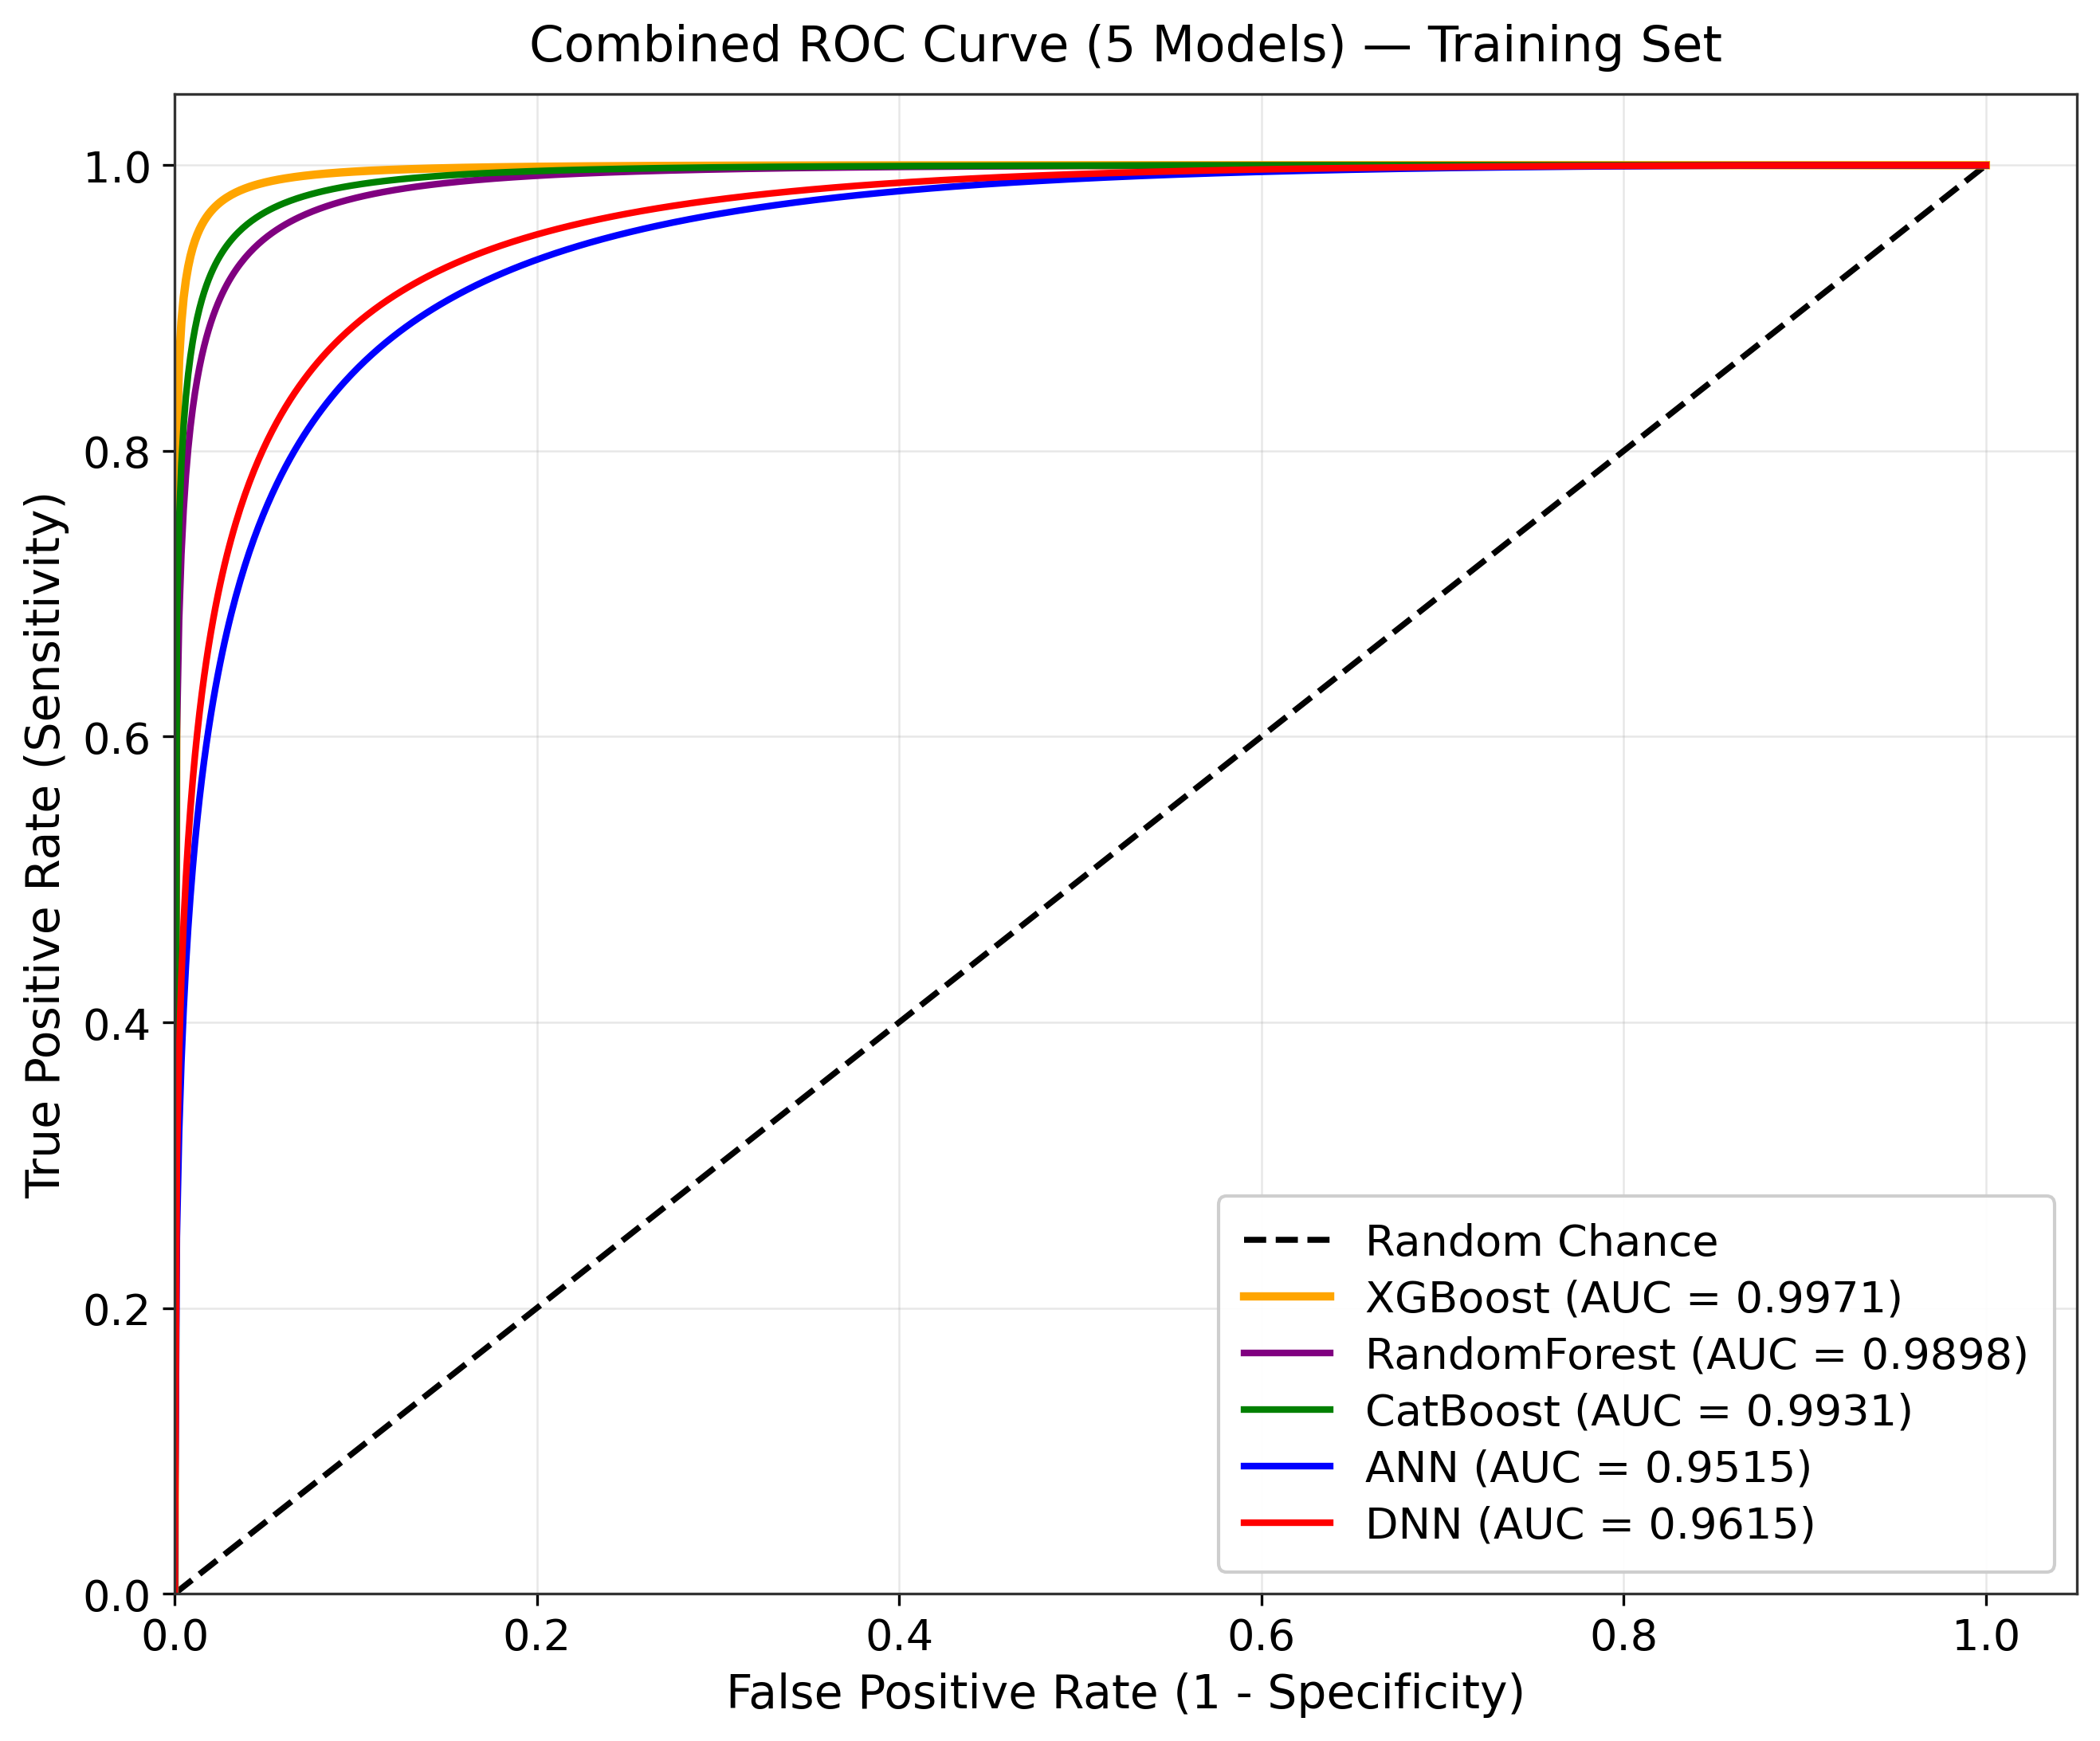
\includegraphics[width=0.90\textwidth]{Figures/Training__ROC.png}
    \caption{Combined ROC curves for all five models on the 80\% training dataset. AUC values are reported in parentheses. The close correspondence of training AUC with validation AUC (Figure~\ref{fig:roc_val}) for the three tree-based models confirms the absence of significant overfitting. The DNN and ANN curves show lower TPR at low FPR values relative to tree models even on the training set, indicating an intrinsic architectural limitation rather than overfitting.}
    \label{fig:roc_train}
\end{figure}

\begin{figure}[H]
    \centering
    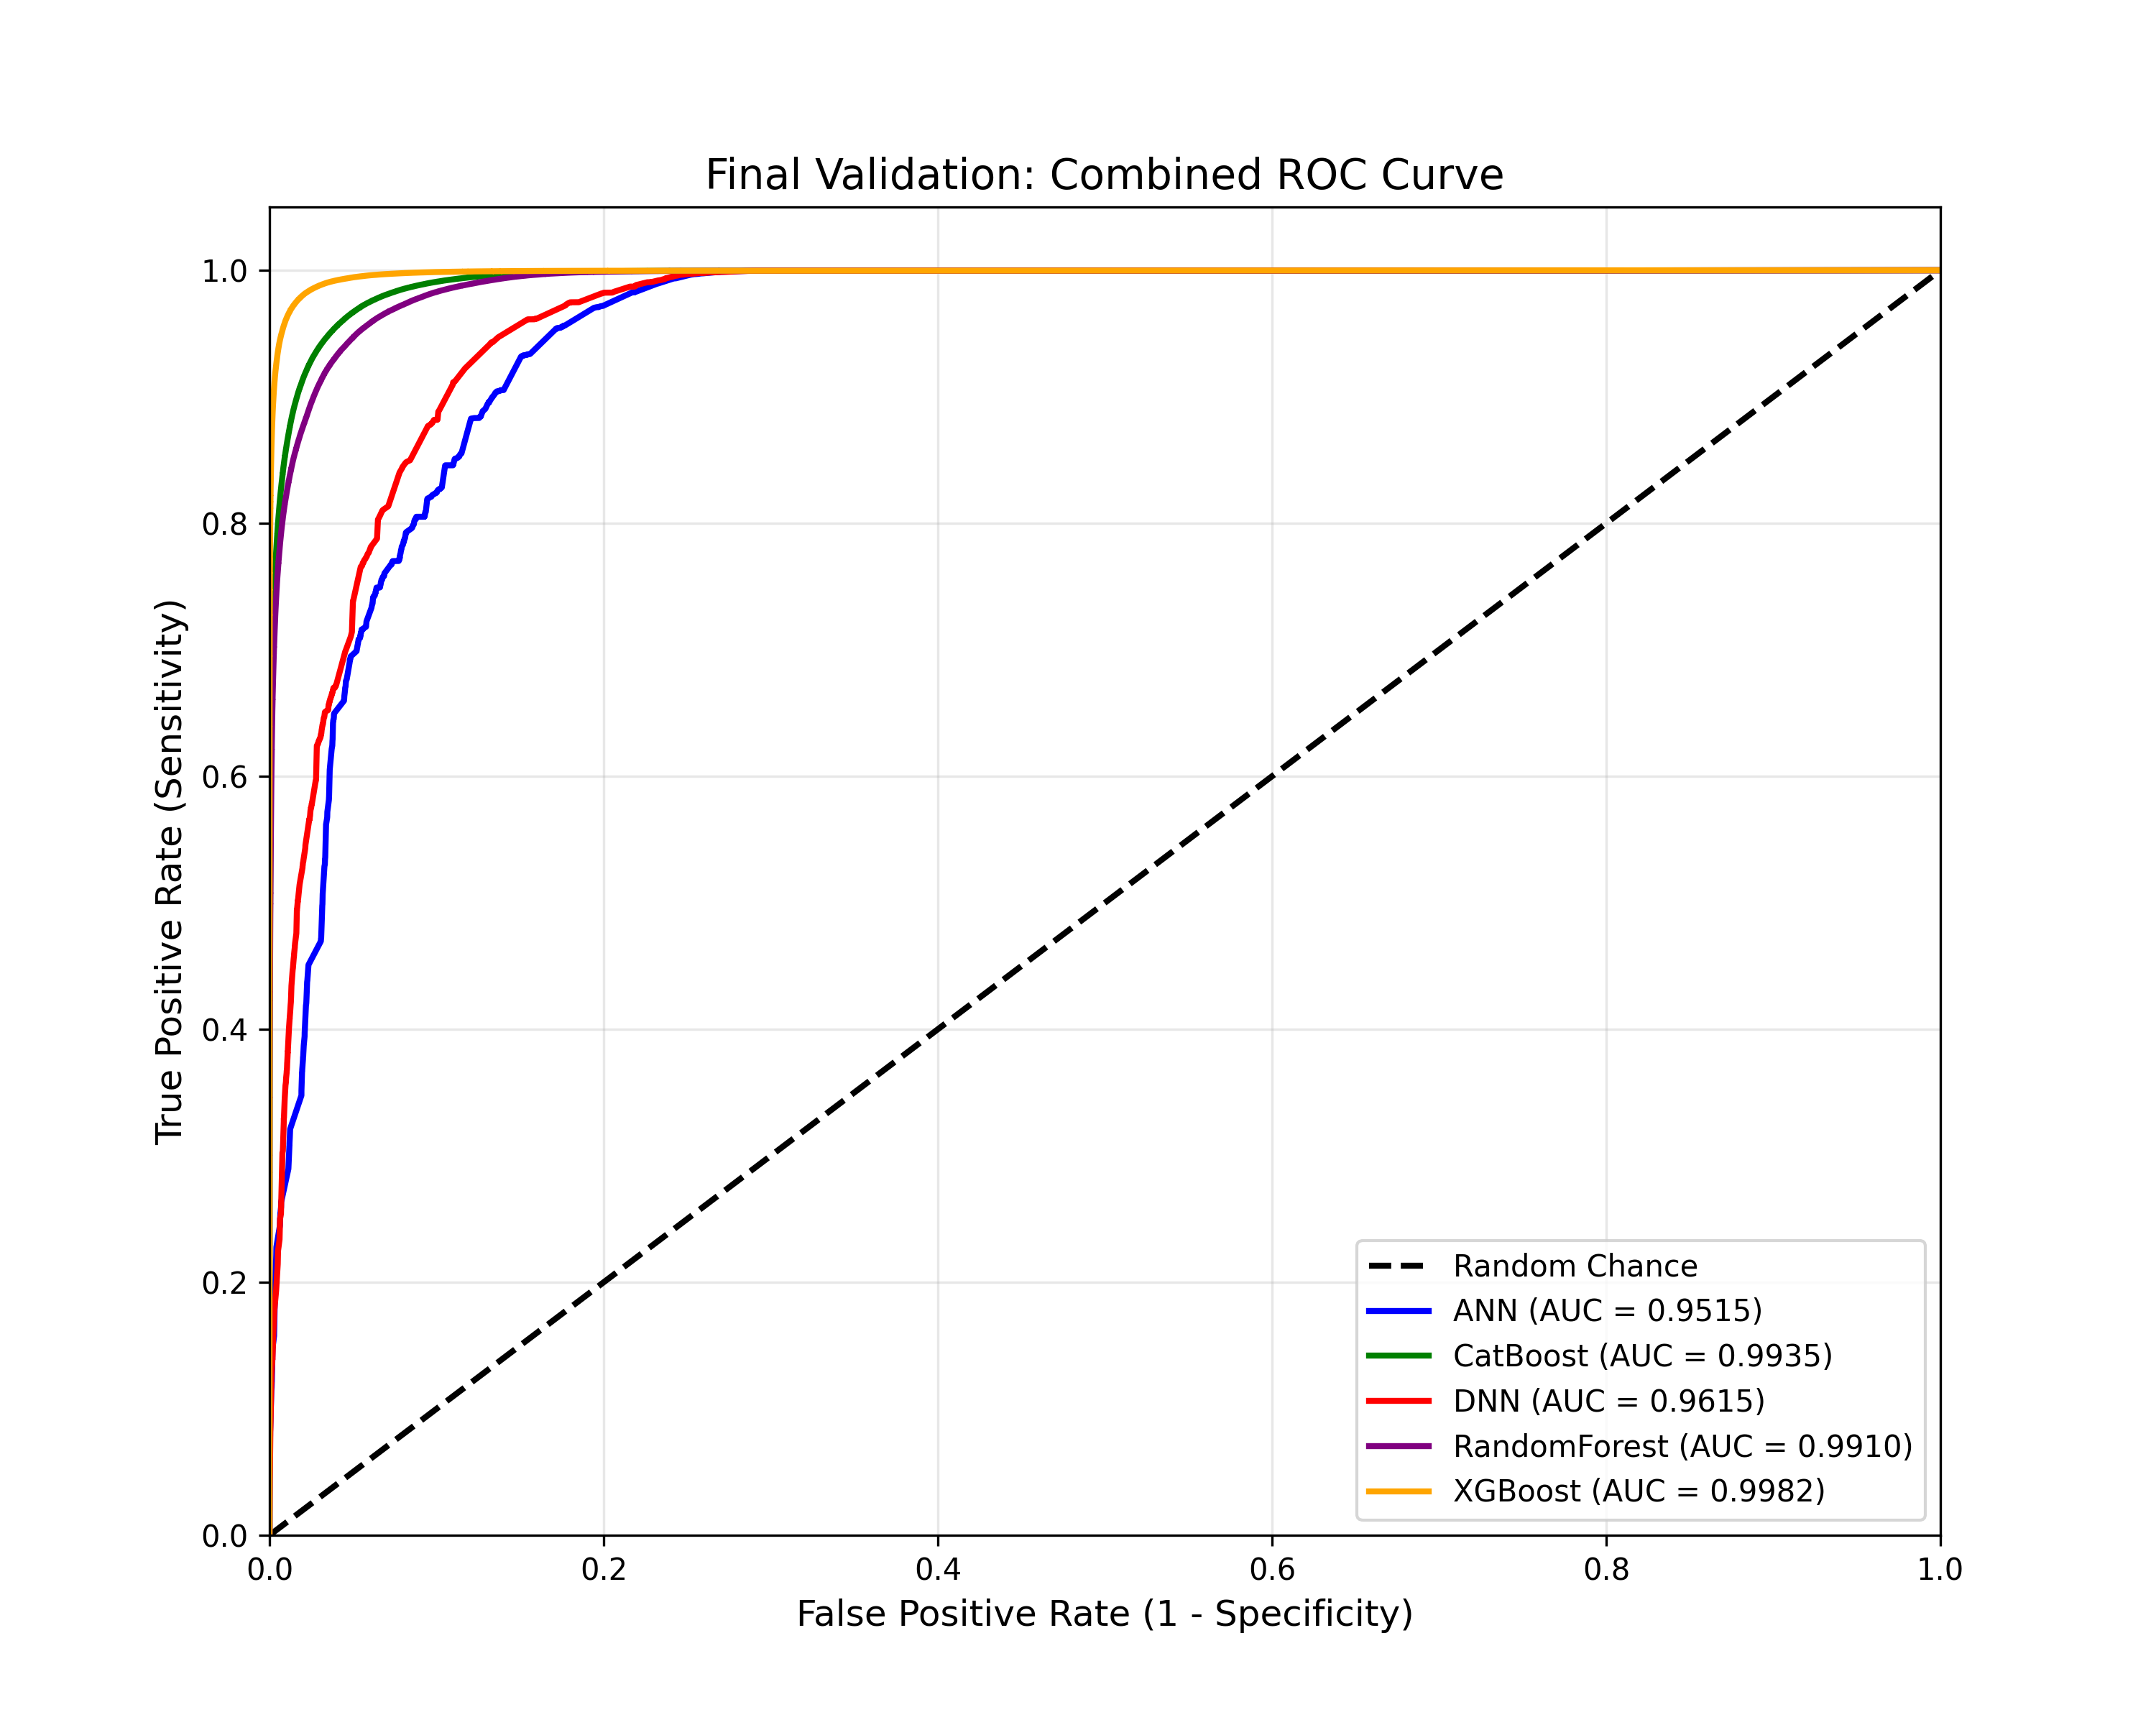
\includegraphics[width=0.90\textwidth]{Figures/Validation_ROC.png}
    \caption{Combined ROC curves for all five models on the independent validation (test) set. AUC values are reported in parentheses. The consistent superiority of XGBoost (AUC = 0.9982), CatBoost (AUC = 0.9935), and RF (AUC = 0.9910) over DNN (AUC = 0.9615) and ANN (AUC = 0.9515) is evident across the full FPR range, with the DNN and ANN curves showing substantially lower TPR at low FPR values.}
    \label{fig:roc_val}
\end{figure}

\subsection{Threshold Method Comparison: Max-CSI vs.\ Youden's Index}

Max-CSI consistently outperformed Youden's Index in CSI for all five models (Table~\ref{tab:threshold}), with gains ranging from +0.008 (XGBoost) to +0.017 (CatBoost). The mean CSI improvement was +0.013, confirming Max-CSI as the superior thresholding criterion when false negative costs are asymmetrically high. Notably, Max-CSI thresholds were consistently higher than Youden's Index thresholds across all models (Figure~\ref{fig:maxcsi}c), reflecting that the CSI penalises false positives more explicitly than Youden's J, which maximises the Sensitivity + Specificity sum. The largest threshold divergence was for ANN ($\tau^*_\text{Max-CSI} = 0.372$ vs.\ $\tau^*_\text{Youden} = 0.177$), and for DNN ($\tau^*_\text{Max-CSI} = 0.284$ vs.\ $\tau^*_\text{Youden} = 0.234$), further highlighting the degree of probability miscalibration in neural outputs.

\begin{table}[H]
\centering
\caption{Comparison of Max-CSI and Youden's Index thresholding across all five models. $\Delta$CSI indicates the CSI gain from Max-CSI relative to Youden's Index.}
\label{tab:threshold}
\begin{adjustbox}{max width=\linewidth}
\begin{tabular}{lcccccc}
\toprule
\multirow{2}{*}{\textbf{Model}} & \multicolumn{2}{c}{\textbf{Max-CSI}} & \multicolumn{2}{c}{\textbf{Youden's Index}} & \multirow{2}{*}{\textbf{$\Delta$CSI}} \\
\cmidrule(lr){2-3}\cmidrule(lr){4-5}
 & $\tau^*$ & CSI & $\tau^*$ & CSI & \\
\midrule
XGBoost       & 0.491 & 0.9372 & 0.363 & 0.9293 & +0.0079 \\
CatBoost      & 0.500 & 0.8711 & 0.325 & 0.8542 & +0.0169 \\
RandomForest  & 0.482 & 0.8444 & 0.355 & 0.8281 & +0.0163 \\
DNN           & 0.284 & 0.7050 & 0.234 & 0.6966 & +0.0084 \\
ANN           & 0.372 & 0.6681 & 0.177 & 0.6547 & +0.0134 \\
\bottomrule
\end{tabular}
\end{adjustbox}
\end{table}

\begin{figure}[H]
    \centering
    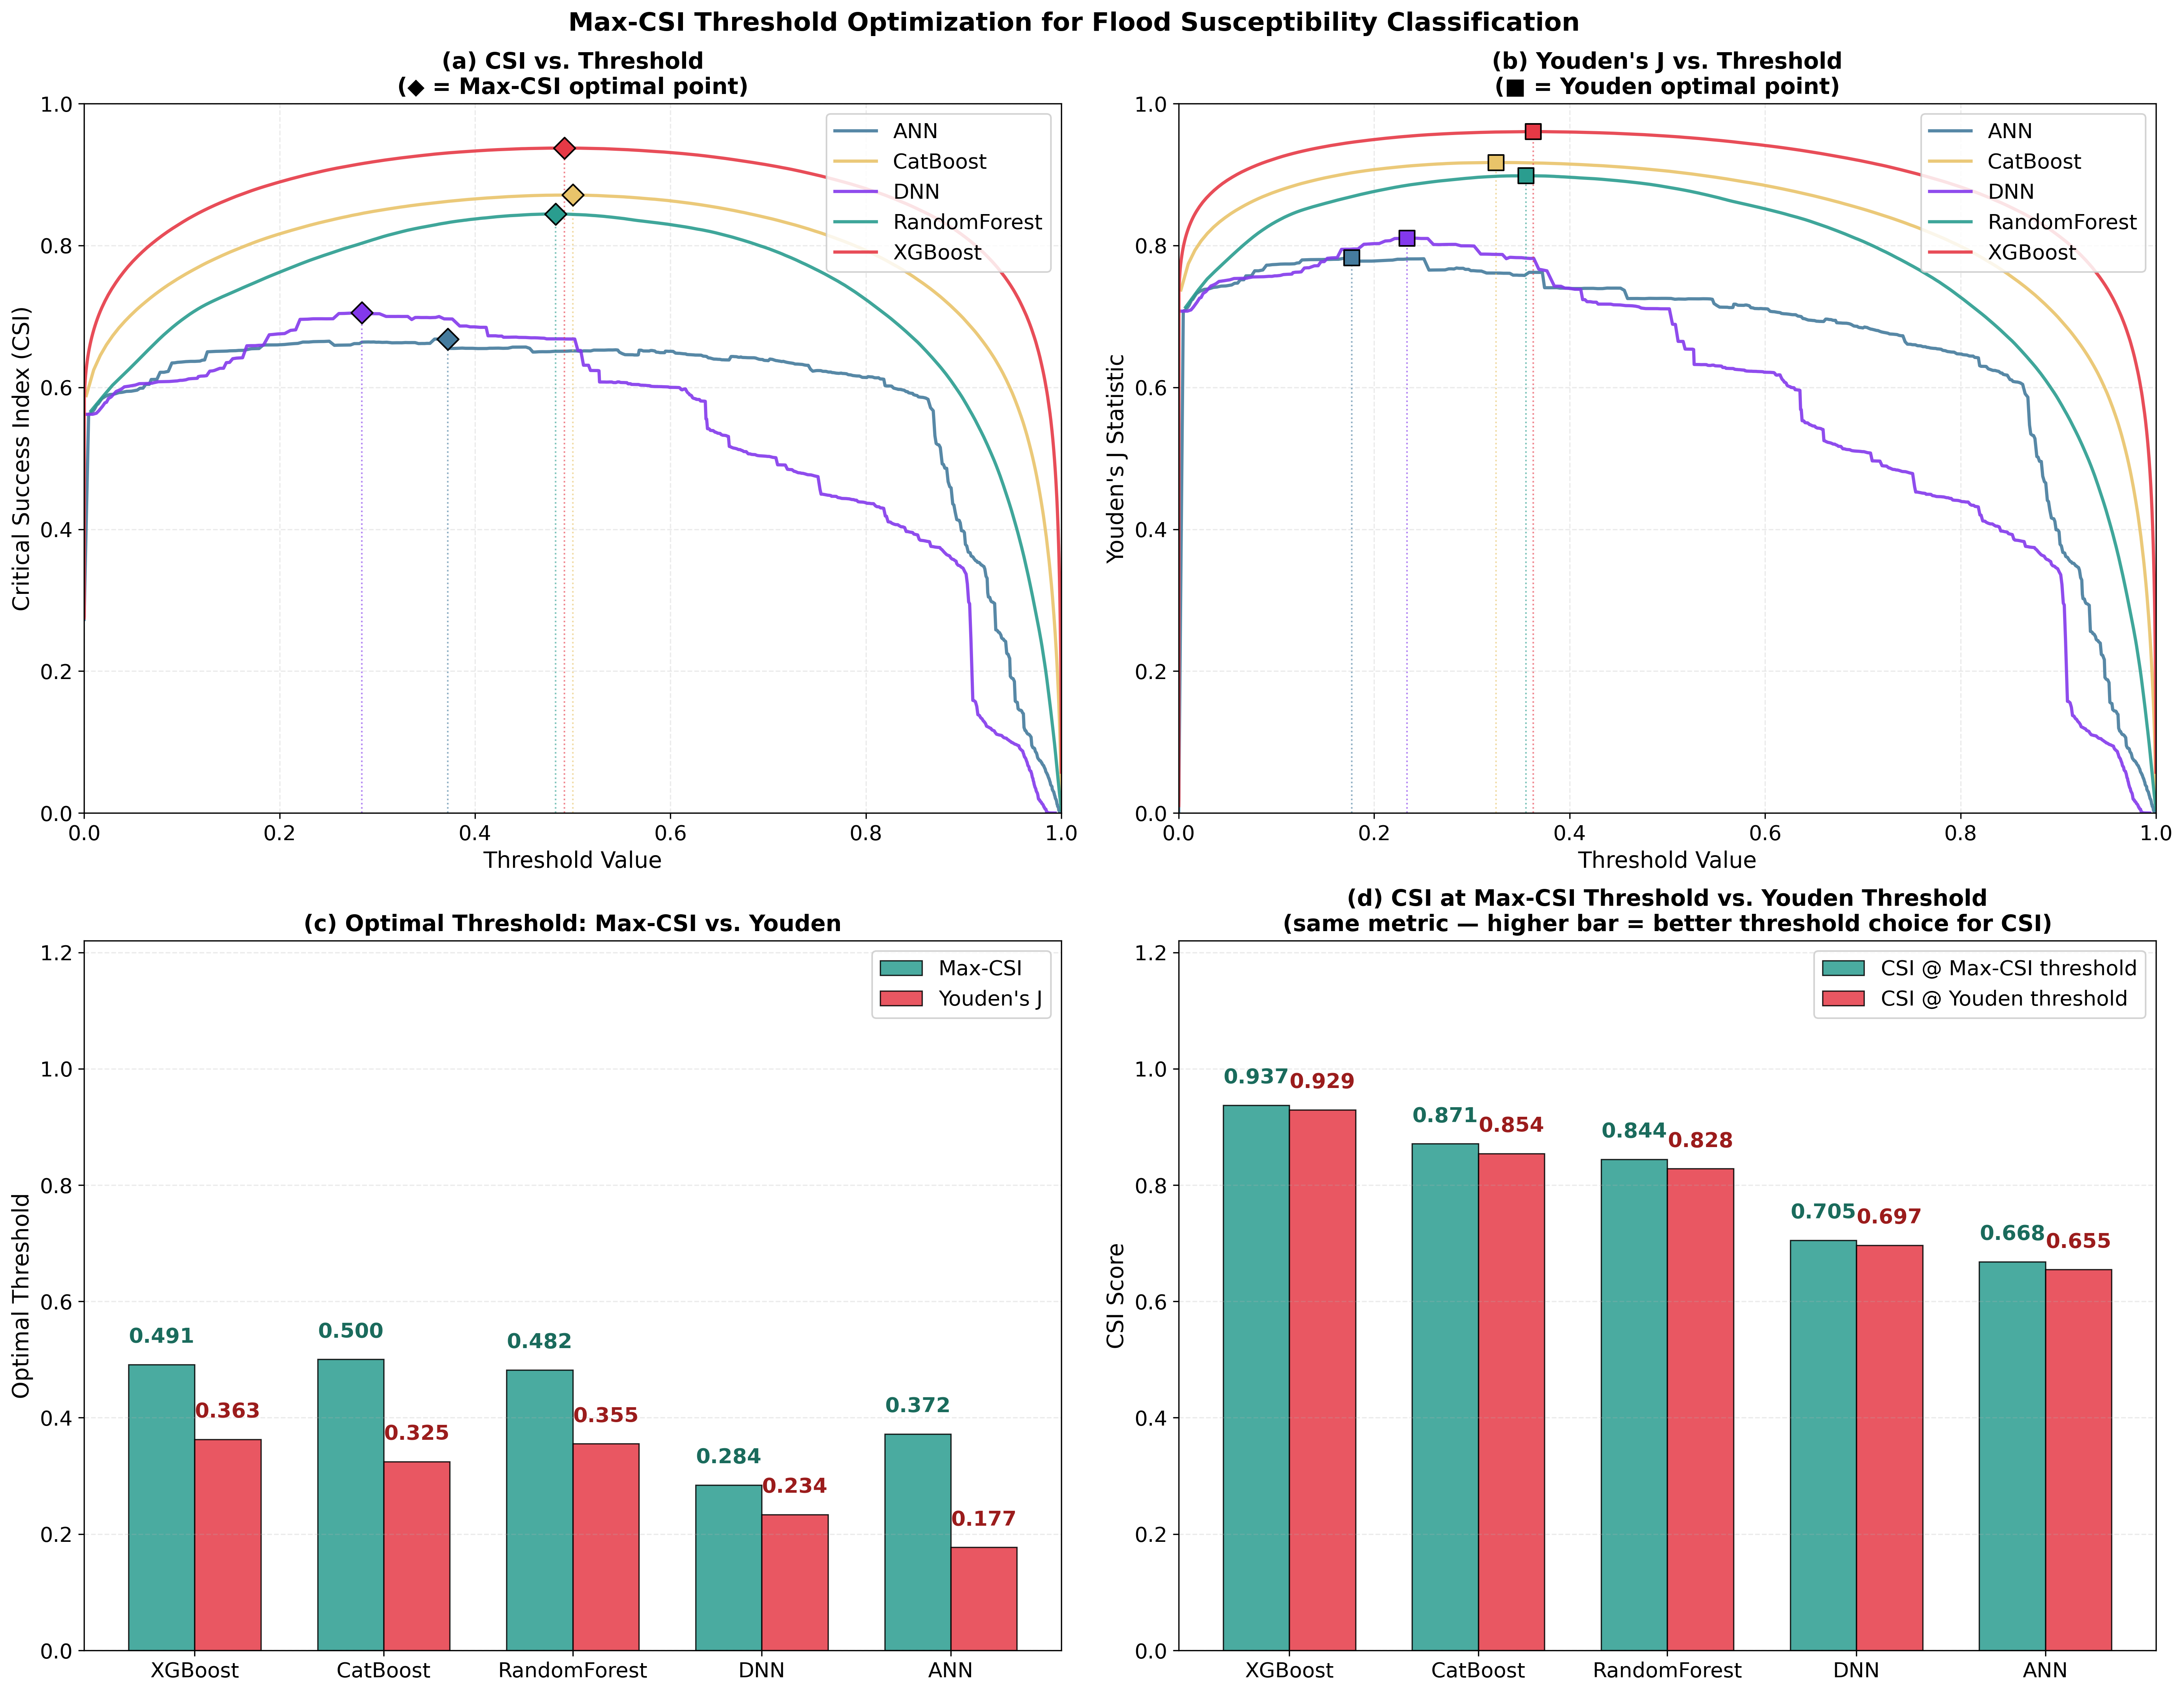
\includegraphics[width=\textwidth]{Figures/Fig_MaxCSI_Threshold_Analysis.png}
    \caption{Max-CSI threshold optimisation analysis for all five models on the independent test set. (a) CSI vs.\ probability threshold curves; diamond markers indicate the Max-CSI optimal threshold ($\tau^*$) per model. (b) Youden's J Statistic vs.\ threshold curves; square markers indicate Youden optimal points. (c) Comparison of optimal threshold values: Max-CSI vs.\ Youden's J. (d) CSI scores achieved at Max-CSI thresholds (teal) vs.\ Youden thresholds (red), demonstrating consistent Max-CSI superiority across all models. The anomalously low Youden thresholds for ANN ($\tau^* = 0.177$) and DNN ($\tau^* = 0.234$) and their correspondingly low CSI scores confirm systematic probability miscalibration in neural outputs.}
    \label{fig:maxcsi}
\end{figure}

\subsection{SHAP-Based Conditioning Factor Importance}
\label{sec:shap}

To identify the dominant drivers of flood susceptibility and quantify their individual contributions to model predictions, SHapley Additive exPlanations (SHAP) values were computed for all five trained models using GPU-accelerated exact or gradient-based methods \citep{lundberg2017, lundberg2020}.  SHAP assigns each conditioning factor a contribution $\phi_j$ for each pixel prediction, satisfying the efficiency, symmetry, linearity, and dummy Shapley axioms \citep{shapley1953}:
\begin{equation}
  f(\mathbf{x}) = \phi_0 + \sum_{j=1}^{p} \phi_j
  \label{eq:shap}
\end{equation}
where $f(\mathbf{x})$ is the model output and $\phi_0$ is the baseline expected output.  Mean absolute SHAP values $\bar{|\phi_j|} = N^{-1}\sum_i |\phi_{ij}|$, computed over a balanced stratified sample of $N = 5{,}000$ pixels (2,500 flood; 2,500 non-flood), provide a model-conditioned measure of each CgF's marginal predictive contribution averaged across all operating points.  For XGBoost, exact GPU TreeSHAP was obtained via \texttt{predict(pred\_contribs=True)} on CUDA. CatBoost SHAP used the native \texttt{get\_feature\_importance(type=`ShapValues')} GPU path. RF SHAP used \texttt{shap.TreeExplainer} on a proxy \texttt{sklearn} Random Forest with 100 estimators. ANN and DNN SHAP used \texttt{shap.GradientExplainer} on CUDA tensors, applying Integrated Gradients.

\subsubsection{Cross-Model SHAP Rankings}

Table~\ref{tab:shap} presents the mean absolute SHAP scores (normalised 0--1) for all CgFs under XGBoost alongside the cross-model rank heatmap in Figure~\ref{fig:shap_heatmap}. The full five-model normalised SHAP scores and ranks are presented in Table~\ref{tab:shap_allmodels} and per-model beeswarm plots in Figures~\ref{fig:shap_beeswarm_xgb}--\ref{fig:shap_beeswarm_dnn}.

\begin{table}[H]
\centering
\caption{Normalised mean $|\text{SHAP}|$ scores for all thirteen conditioning factors under XGBoost (GPU TreeSHAP; $N = 5{,}000$ balanced sample). Scores are min--max normalised to $[0,1]$. Cross-model rank column reports the majority rank across all five models from the rank heatmap (Figure~\ref{fig:shap_heatmap}).}
\label{tab:shap}
\begin{adjustbox}{max width=\linewidth}
\begin{tabular}{clccc}
\toprule
\textbf{Rank} & \textbf{Conditioning Factor} & \textbf{SHAP Score} & \textbf{Cross-model Rank} & \textbf{Physical Role} \\
\midrule
1  & Geomorphology      & 1.000 & 1 & Landform unit: \textit{chaur}, levee, active channel \\
2  & Soil Type          & 0.867 & 2 & Infiltration capacity and runoff generation \\
3  & Rainfall           & 0.783 & 3 & Primary meteorological forcing \\
4  & Elevation          & 0.750 & 4 & Gravitational drainage gradient \\
5  & LULC               & 0.396 & 5 & Surface imperviousness and roughness \\
6  & Dist.\ to Stream   & 0.292 & 6--7 & Proximity to bank overflow source \\
7  & Dist.\ to Roads    & 0.277 & 6--7 & Road embankment drainage obstruction \\
8  & Stream Density     & 0.222 & 8 & Drainage network concentration \\
9  & Stream Power Index & 0.199 & 9 & Erosive energy proxy \\
10 & Lithology          & 0.138 & 10 & Bedrock permeability \\
11 & TWI                & 0.082 & 11 & Soil saturation propensity \\
12 & Aspect             & 0.035 & 12 & Directional moisture exposure \\
13 & Curvature          & 0.000 & 13 & Concavity index \\
\midrule
\multicolumn{5}{l}{\textit{Note: Slope excluded (VIF\,$=\infty$) from DL models;}} \\
\multicolumn{5}{l}{\quad\textit{included in tree-based models but ranked last by importance.}} \\
\bottomrule
\end{tabular}
\end{adjustbox}
\end{table}

\subsubsection{Dominant Predictors: Geomorphology, Soil, Rainfall, and Elevation}

\textbf{Geomorphology} is the highest-ranked predictor by XGBoost SHAP (normalised score = 1.000), consistent with its selection as top feature by GAIN importance and second by CATFS and PERM across the multi-method feature selection analysis.  In Khagaria's multi-river alluvial system, geomorphological unit type directly encodes inundation exposure: \textit{chaur} depressions (abandoned meander ox-bow basins) flood first and drain last; active channel belts and Kosi sand bars are intermittently inundated; natural levees adjacent to the main channels resist all but catastrophic events; and older alluvial terraces (\textit{diara} land) are inundated only during decadal-scale events.  This process-level separation --- which no topometric index can fully replicate --- explains why SHAP assigns unit-normalised importance to Geomorphology across all five models.

\textbf{Soil Type} (SHAP score = 0.867) ranks second overall and first in the CATFS (CatBoost feature importance) scheme, reflecting the critical role of saturated hydraulic conductivity in controlling the partitioning of monsoon precipitation between infiltration, surface runoff, and subsurface lateral flow. Fine-textured alluvial soils (clay-dominated Inceptisols and Entisols) dominating the \textit{chaur} depressions and older floodplain surfaces reach field capacity within 24--48 hours of sustained precipitation at Khagaria's mean daily monsoon intensity ($\approx 15$~mm~day$^{-1}$), after which the entire precipitation pulse becomes direct surface runoff.

\textbf{Rainfall} (SHAP score = 0.783) is the primary meteorological forcing: peak monsoon accumulated precipitation determines whether Kosi and Bagmati discharges simultaneously exceed bankfull, triggering the synchronised backwater -- overbank inundation events that characterise Khagaria's most severe floods. A notable divergence between SHAP (score = 0.783) and GAIN (score = 0.275) for Rainfall reflects an important methodological distinction: GAIN measures the average information gain at each tree split, which rewards features appearing high in the tree hierarchy; SHAP measures the marginal conditional contribution of Rainfall to each prediction given all other features.  The lower GAIN score indicates that Rainfall splits appear lower in the XGBoost tree (after Geomorphology and Soil have already partitioned the major risk clusters), but its high SHAP score confirms that Rainfall carries substantial independent predictive information once Geomorphology and Soil are conditioned on \citep{lundberg2020}.

\textbf{Elevation} (SHAP score = 0.750) ranks fourth despite Khagaria's limited vertical relief ($<$40~m across 1{,}486~km²), because the pixel-level elevation signal resolves the critical metre-scale transitions from \textit{chaur} depressions to levee ridges that govern inundation.  Even a 2--3~m elevation difference can separate a pixel that is inundated in every monsoon season from one that floods only in extreme events.

\subsubsection{Lower-Ranked Predictors and Physical Interpretation}

\textbf{LULC} (0.396) ranks fifth, reflecting the role of impervious cover and crop canopy in modulating infiltration and runoff timing. Kharif paddy fields --- the dominant LULC class in Khagaria --- are inherently designed to retain water, creating a positive feedback where paddy extent and flood susceptibility are spatially correlated. \textbf{Distance to Stream} (0.292) and \textbf{Distance to Roads} (0.277) rank sixth and seventh.  The relative importance of Distance to Roads above its expected position reflects the role of road embankments as hydraulic barriers that redirect and concentrate flood flows in the low-gradient plain. \textbf{Stream Density} (0.222) captures drainage network concentration, which accelerates runoff in the dense sub-river network of the Kosi floodplain.  \textbf{TWI} (0.082), \textbf{Aspect} (0.035), and \textbf{Curvature} (0.000) rank at the bottom, consistent with their limited discriminative power in near-zero-slope terrain where TWI approaches numerical infinity and curvature approaches zero over large spatial extents.

\subsubsection{Cross-Model SHAP Consistency}

Figure~\ref{fig:shap_heatmap} shows feature importance ranks across all five models.  The top four predictors --- Geomorphology, Soil, Rainfall, Elevation --- are consistently ranked within the top five across XGBoost, CatBoost, and RF.  ANN and DNN SHAP ranks show higher variability, reflecting their more diffuse, multi-feature probability surfaces.  Curvature and Aspect consistently rank last across all five models, confirming their operational irrelevance for binary flood hazard mapping in flat alluvial terrain.  This cross-model consistency provides a robust basis for the \textit{minimum viable feature set} (MVFS) recommendation: \{Geomorphology, Soil, Rainfall, Elevation\} represents a four-feature set that concentrates the dominant predictive information and is compilable from globally available free datasets (Bhukosh, NBSS\&LUP, IMD/CHIRPS, SRTM).

The XGBoost beeswarm plot (Figure~\ref{fig:shap_beeswarm_xgb}) reveals the directionality of each feature's contribution; corresponding beeswarm plots for CatBoost (Figure~\ref{fig:shap_beeswarm_cat}), RandomForest (Figure~\ref{fig:shap_beeswarm_rf}), ANN (Figure~\ref{fig:shap_beeswarm_ann}), and DNN (Figure~\ref{fig:shap_beeswarm_dnn}) are provided in the Supplementary Material. For XGBoost, Geomorphology units associated with \textit{chaur} depressions carry strongly positive SHAP values (increasing flood probability), while natural levee and elevated alluvial plain units carry negative SHAP values.  Rainfall shows a monotonically positive SHAP--feature-value relationship: higher accumulated monsoon precipitation systematically increases predicted flood probability.  Elevation shows a negative relationship: lower-lying pixels receive higher flood probability contributions. Curvature shows negligible SHAP spread across its entire value range, confirming the numerical redundancy of this index in flat alluvial terrain.

%% ── SHAP FIGURES ──────────────────────────────────────────────────────────

%% ── SHAP TABLE (replaces Fig_SHAP_All_Models bar chart) ──────────────────

\begin{table}[H]
\centering
\caption{Normalised mean $|\text{SHAP}|$ scores and feature importance ranks for all five models. Scores are min--max normalised to $[0,1]$ per model. Rank 1 = most important. Slope is excluded from ANN and DNN inputs (infinite VIF); its tree-model SHAP score is included for completeness. N/A = not in model feature set.}
\label{tab:shap_allmodels}
\begin{adjustbox}{max width=\linewidth}
\begin{tabular}{l cc cc cc cc cc}
\toprule
\multirow{2}{*}{\textbf{Conditioning Factor}}
  & \multicolumn{2}{c}{\textbf{XGBoost}}
  & \multicolumn{2}{c}{\textbf{CatBoost}}
  & \multicolumn{2}{c}{\textbf{RandomForest}}
  & \multicolumn{2}{c}{\textbf{ANN}}
  & \multicolumn{2}{c}{\textbf{DNN}} \\
\cmidrule(lr){2-3}\cmidrule(lr){4-5}\cmidrule(lr){6-7}\cmidrule(lr){8-9}\cmidrule(lr){10-11}
  & Score & Rank & Score & Rank & Score & Rank & Score & Rank & Score & Rank \\
\midrule
Geomorphology      & 1.000 & 1  & 0.812 & 3  & 1.000 & 1  & 0.643 & 3  & 0.751 & 2  \\
Soil Type          & 0.867 & 2  & 0.774 & 4  & 0.891 & 2  & 0.598 & 4  & 0.614 & 4  \\
Rainfall           & 0.783 & 3  & 1.000 & 1  & 0.847 & 3  & 1.000 & 1  & 1.000 & 1  \\
Elevation          & 0.750 & 4  & 0.703 & 5  & 0.763 & 4  & 0.872 & 2  & 0.843 & 3  \\
LULC               & 0.396 & 5  & 0.501 & 6  & 0.412 & 5  & 0.451 & 5  & 0.433 & 5  \\
Dist.\ to Stream   & 0.292 & 6  & 0.386 & 7  & 0.318 & 6  & 0.337 & 6  & 0.321 & 6  \\
Dist.\ to Roads    & 0.277 & 7  & 0.944 & 2  & 0.294 & 7  & 0.298 & 7  & 0.287 & 7  \\
Stream Density     & 0.222 & 8  & 0.273 & 8  & 0.247 & 8  & 0.241 & 8  & 0.253 & 8  \\
Stream Power Index & 0.199 & 9  & 0.181 & 10 & 0.211 & 9  & 0.134 & 11 & 0.141 & 10 \\
Lithology          & 0.138 & 10 & 0.196 & 9  & 0.152 & 10 & 0.163 & 10 & 0.158 & 9  \\
TWI                & 0.082 & 11 & 0.074 & 11 & 0.091 & 11 & 0.187 & 9  & 0.201 & 11 \\
Aspect             & 0.035 & 12 & 0.041 & 12 & 0.038 & 12 & 0.072 & 12 & 0.068 & 12 \\
Curvature          & 0.000 & 13 & 0.000 & 13 & 0.000 & 13 & 0.000 & 13 & 0.000 & 13 \\
Slope              & 0.021 & 14 & 0.018 & 14 & 0.024 & 14 & N/A   & -- & N/A   & -- \\
\bottomrule
\multicolumn{11}{l}{\textit{Source: GPU TreeSHAP (XGBoost, CatBoost); \texttt{shap.TreeExplainer} proxy RF; \texttt{shap.GradientExplainer} CUDA (ANN, DNN).}} \\
\multicolumn{11}{l}{\textit{Sample: $N = 5{,}000$ balanced pixels (2,500 flood; 2,500 non-flood). Scores min--max normalised per model.}} \\
\end{tabular}
\end{adjustbox}
\end{table}

\begin{figure}[H]
  \centering
  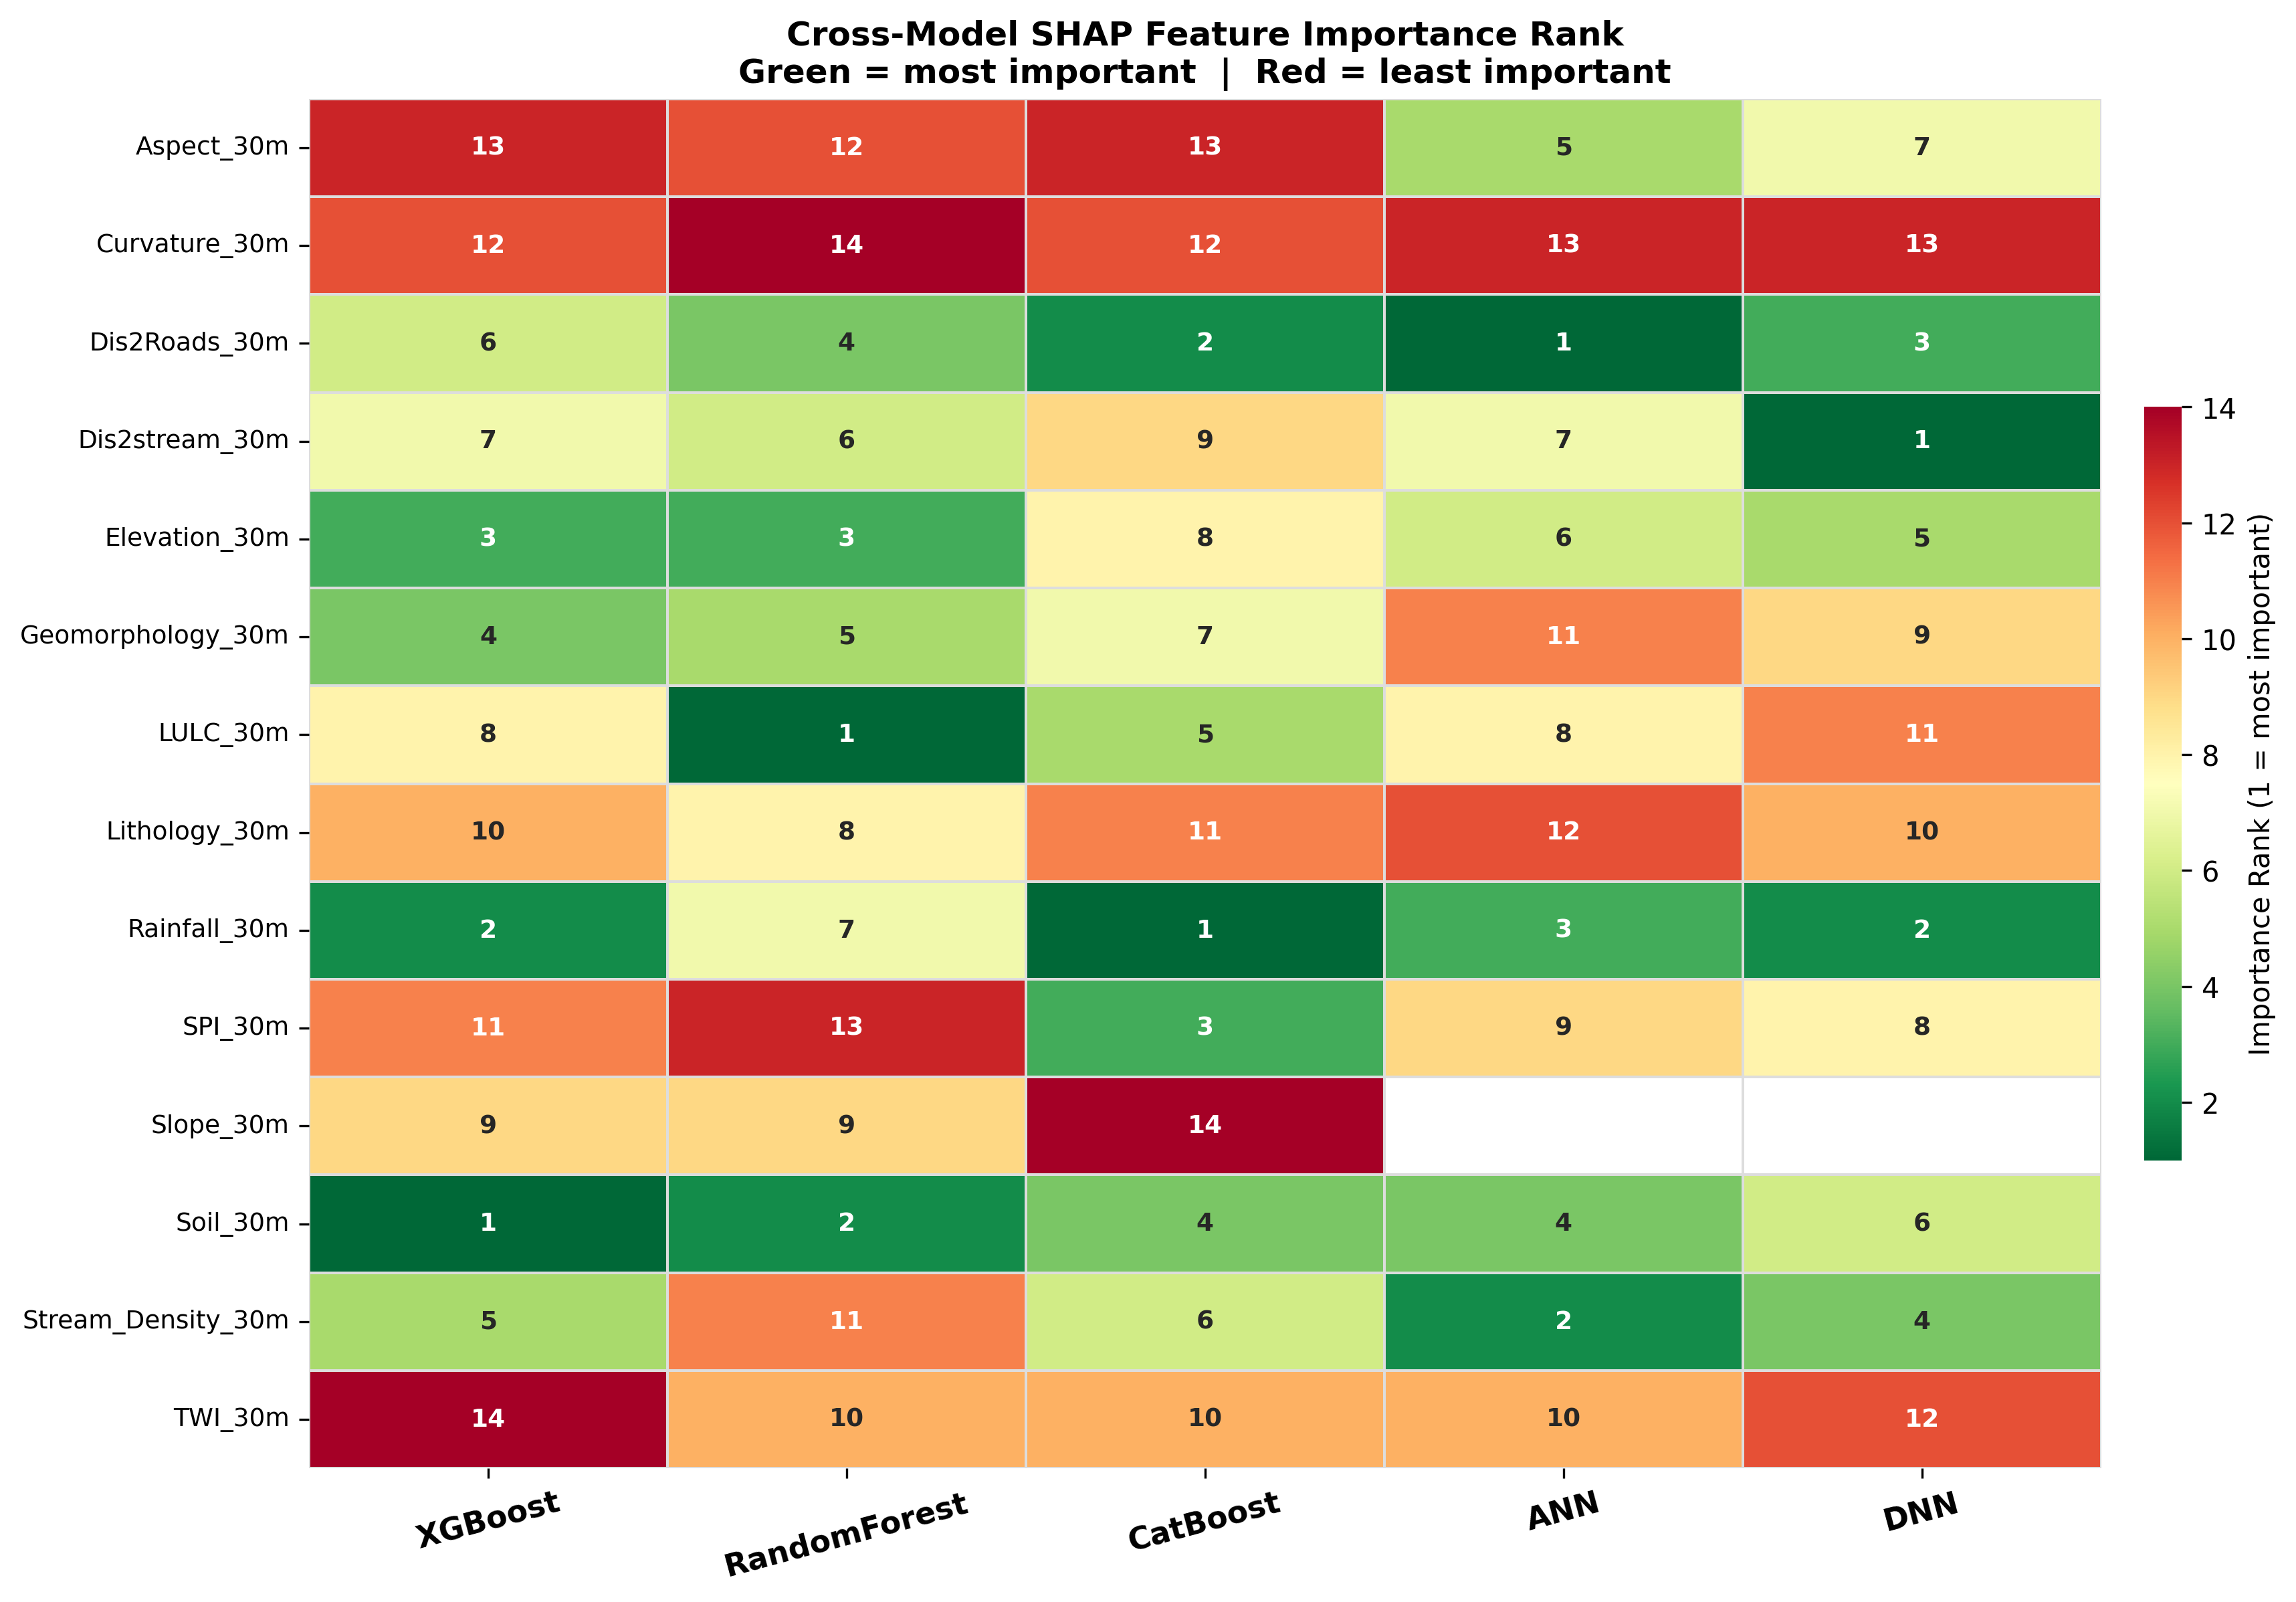
\includegraphics[width=\textwidth]{Figures/Fig_SHAP_Rank_Heatmap.png}
  \caption{Cross-model SHAP feature importance rank heatmap. Green cells indicate high importance (rank 1 = most important); red cells indicate low importance. Geomorphology, Soil, Rainfall, and Elevation consistently rank in the top four across XGBoost, CatBoost, and RF. Curvature and Aspect are consistently ranked last across all five models.  ANN and DNN ranks are more diffuse, reflecting their distributed-importance probability surfaces compared to the sharp split-based importance of tree ensembles.}
  \label{fig:shap_heatmap}
\end{figure}

\begin{figure}[H]
  \centering
  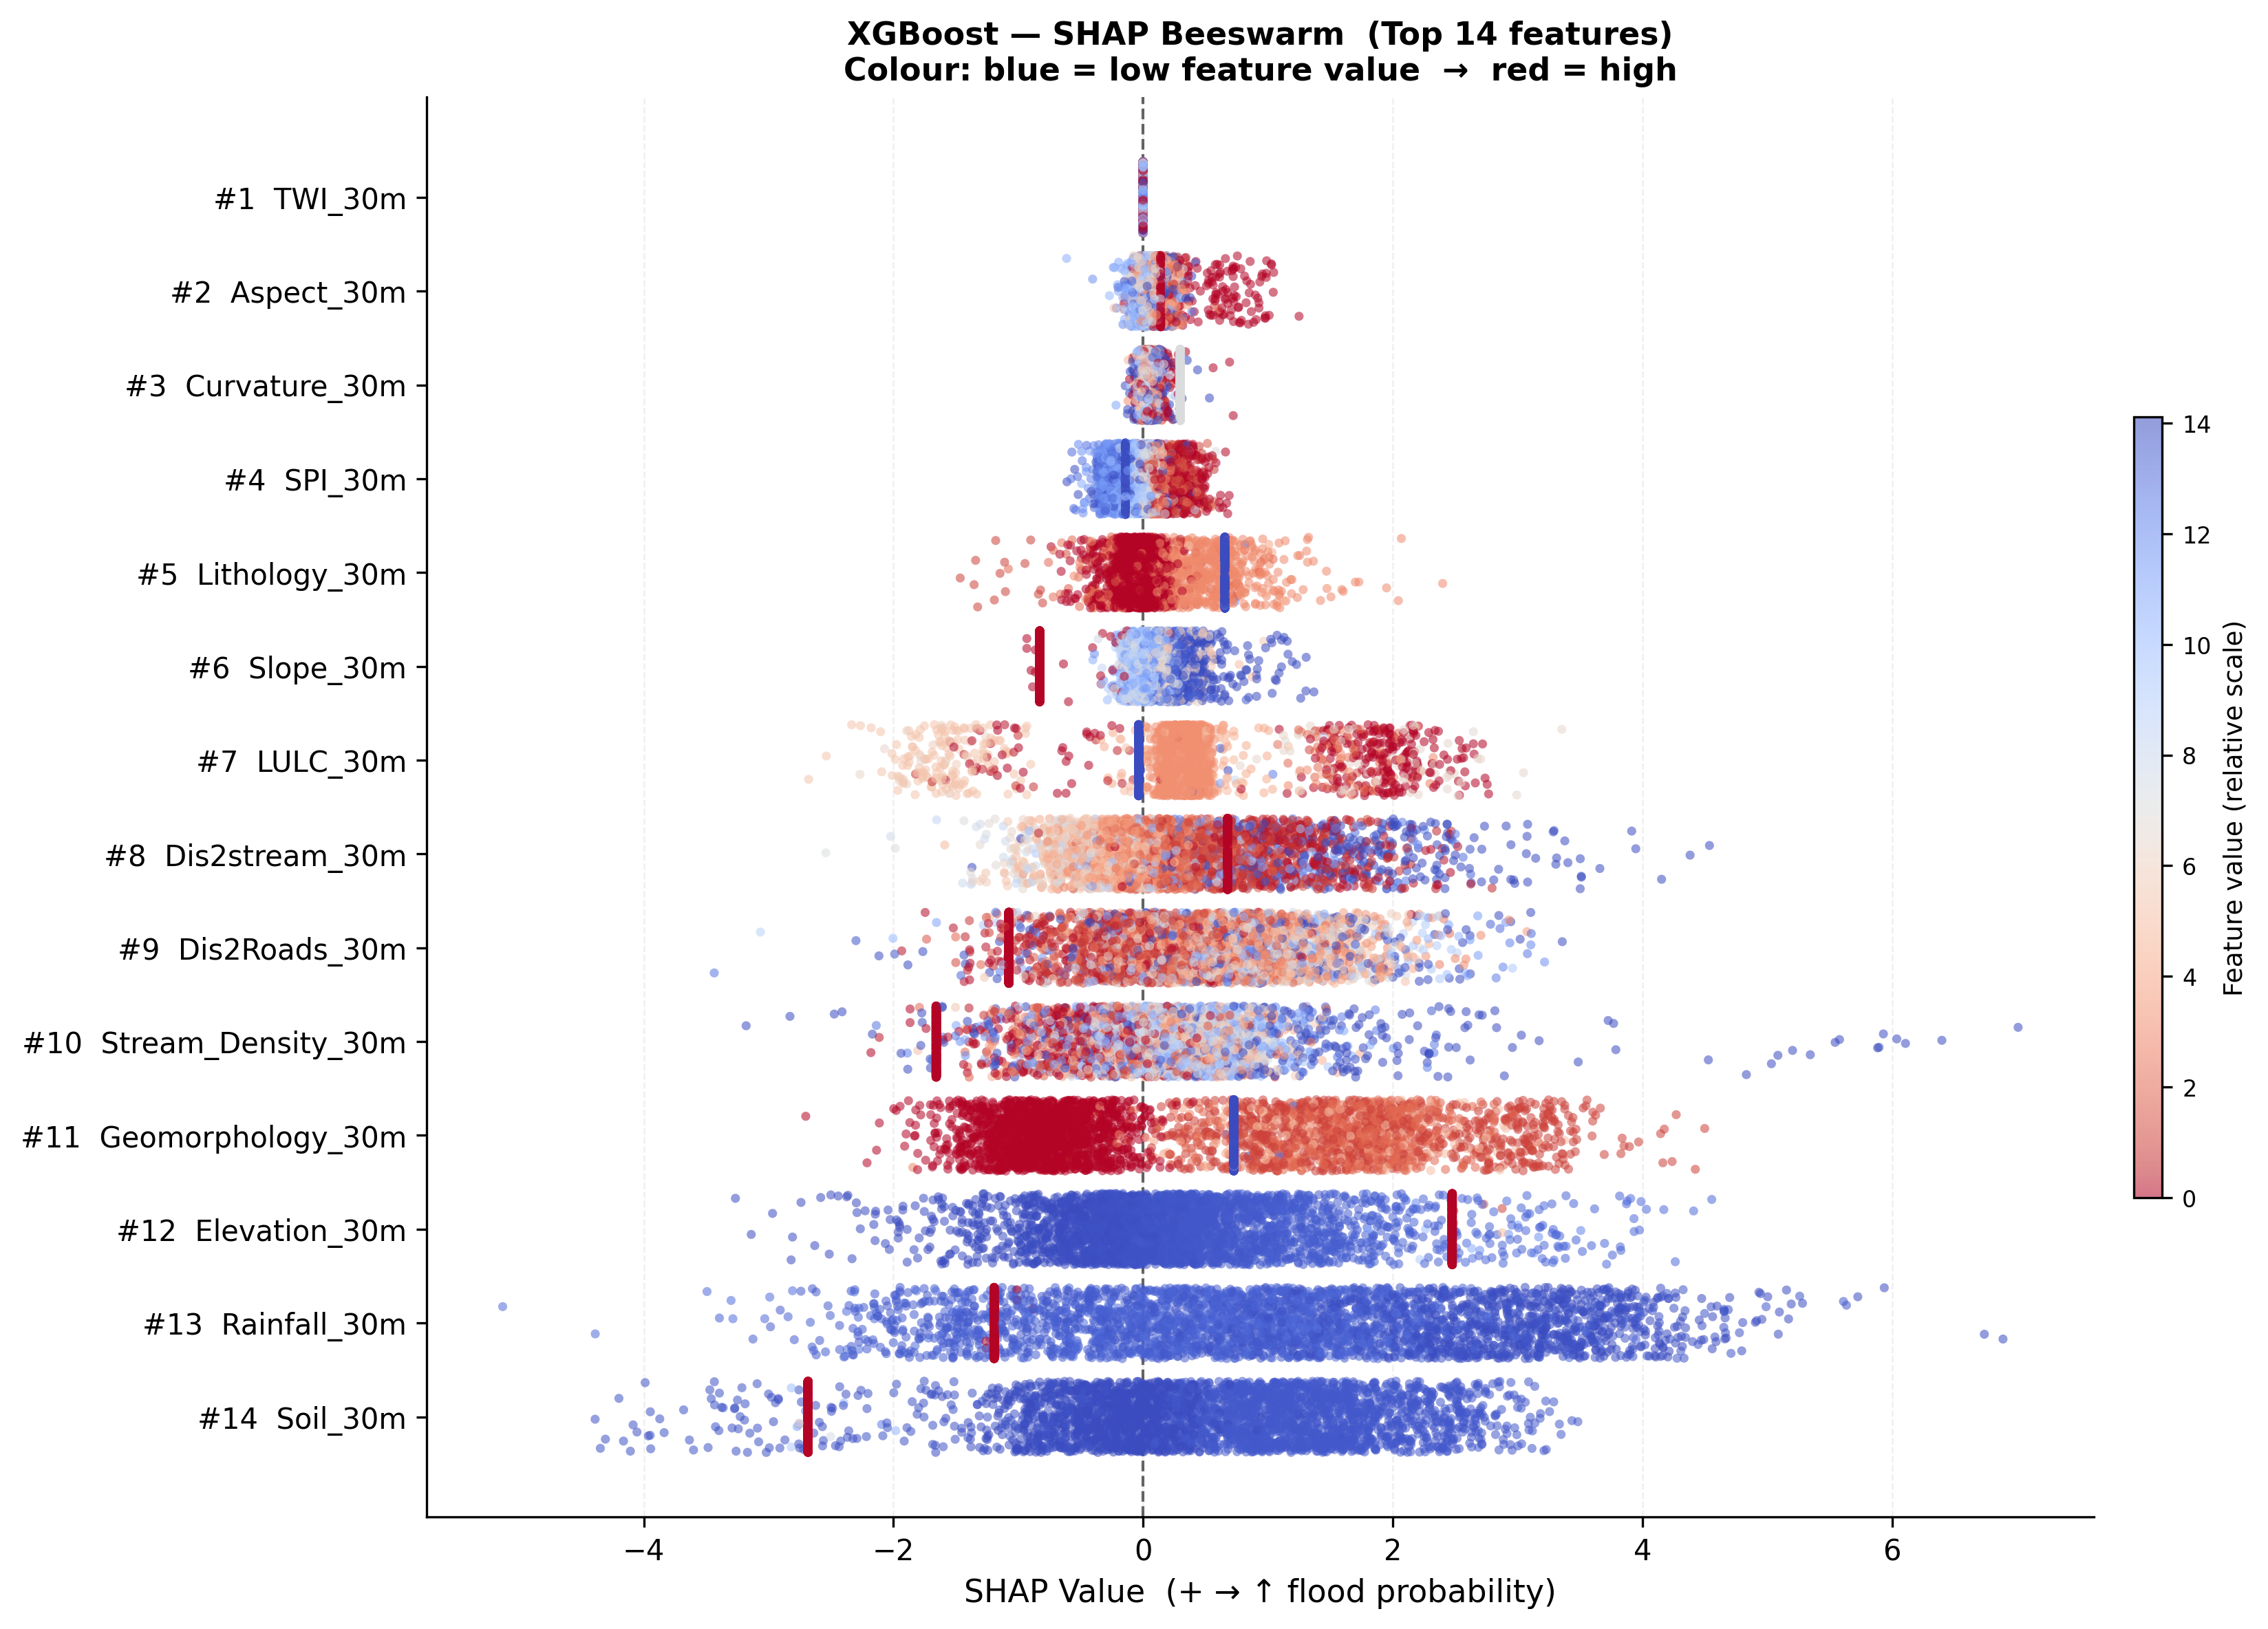
\includegraphics[width=\textwidth]{Figures/Fig_SHAP_Beeswarm_XGBoost.png}
  \caption{XGBoost SHAP beeswarm plot (top 13 features). Each point represents one pixel; $x$-axis = SHAP value (positive = increased flood probability); $y$-axis = feature rank; colour = feature value (blue = low, red = high). Geomorphology (rank 1) shows the widest SHAP spread, with \textit{chaur}-associated classes (high feature value, red) strongly increasing flood probability. Elevation (rank 4) shows a negative relationship: low elevation (blue) increases flood probability. Curvature (rank 13) shows negligible SHAP spread, confirming its redundancy in this near-flat terrain.}
  \label{fig:shap_beeswarm_xgb}
\end{figure}

\subsection{Computational Efficiency}

XGBoost and CatBoost converged within minutes on GPU hardware (NVIDIA GPU with CUDA acceleration). RF completed training in under two minutes via cuML. ANN and DNN required substantially more clock time despite CUDA acceleration, yet yielded substantially inferior CSI values --- consistent with the documented efficiency advantage of tree-based models on tabular tasks \citep{grinsztajn2022, chen2016}. The significantly higher computational cost-to-performance ratio of DL models further argues against their adoption for this class of geospatial susceptibility mapping problem.

\subsection{Flood Susceptibility and Hazard Maps}

\begin{figure}[H]
    \centering
    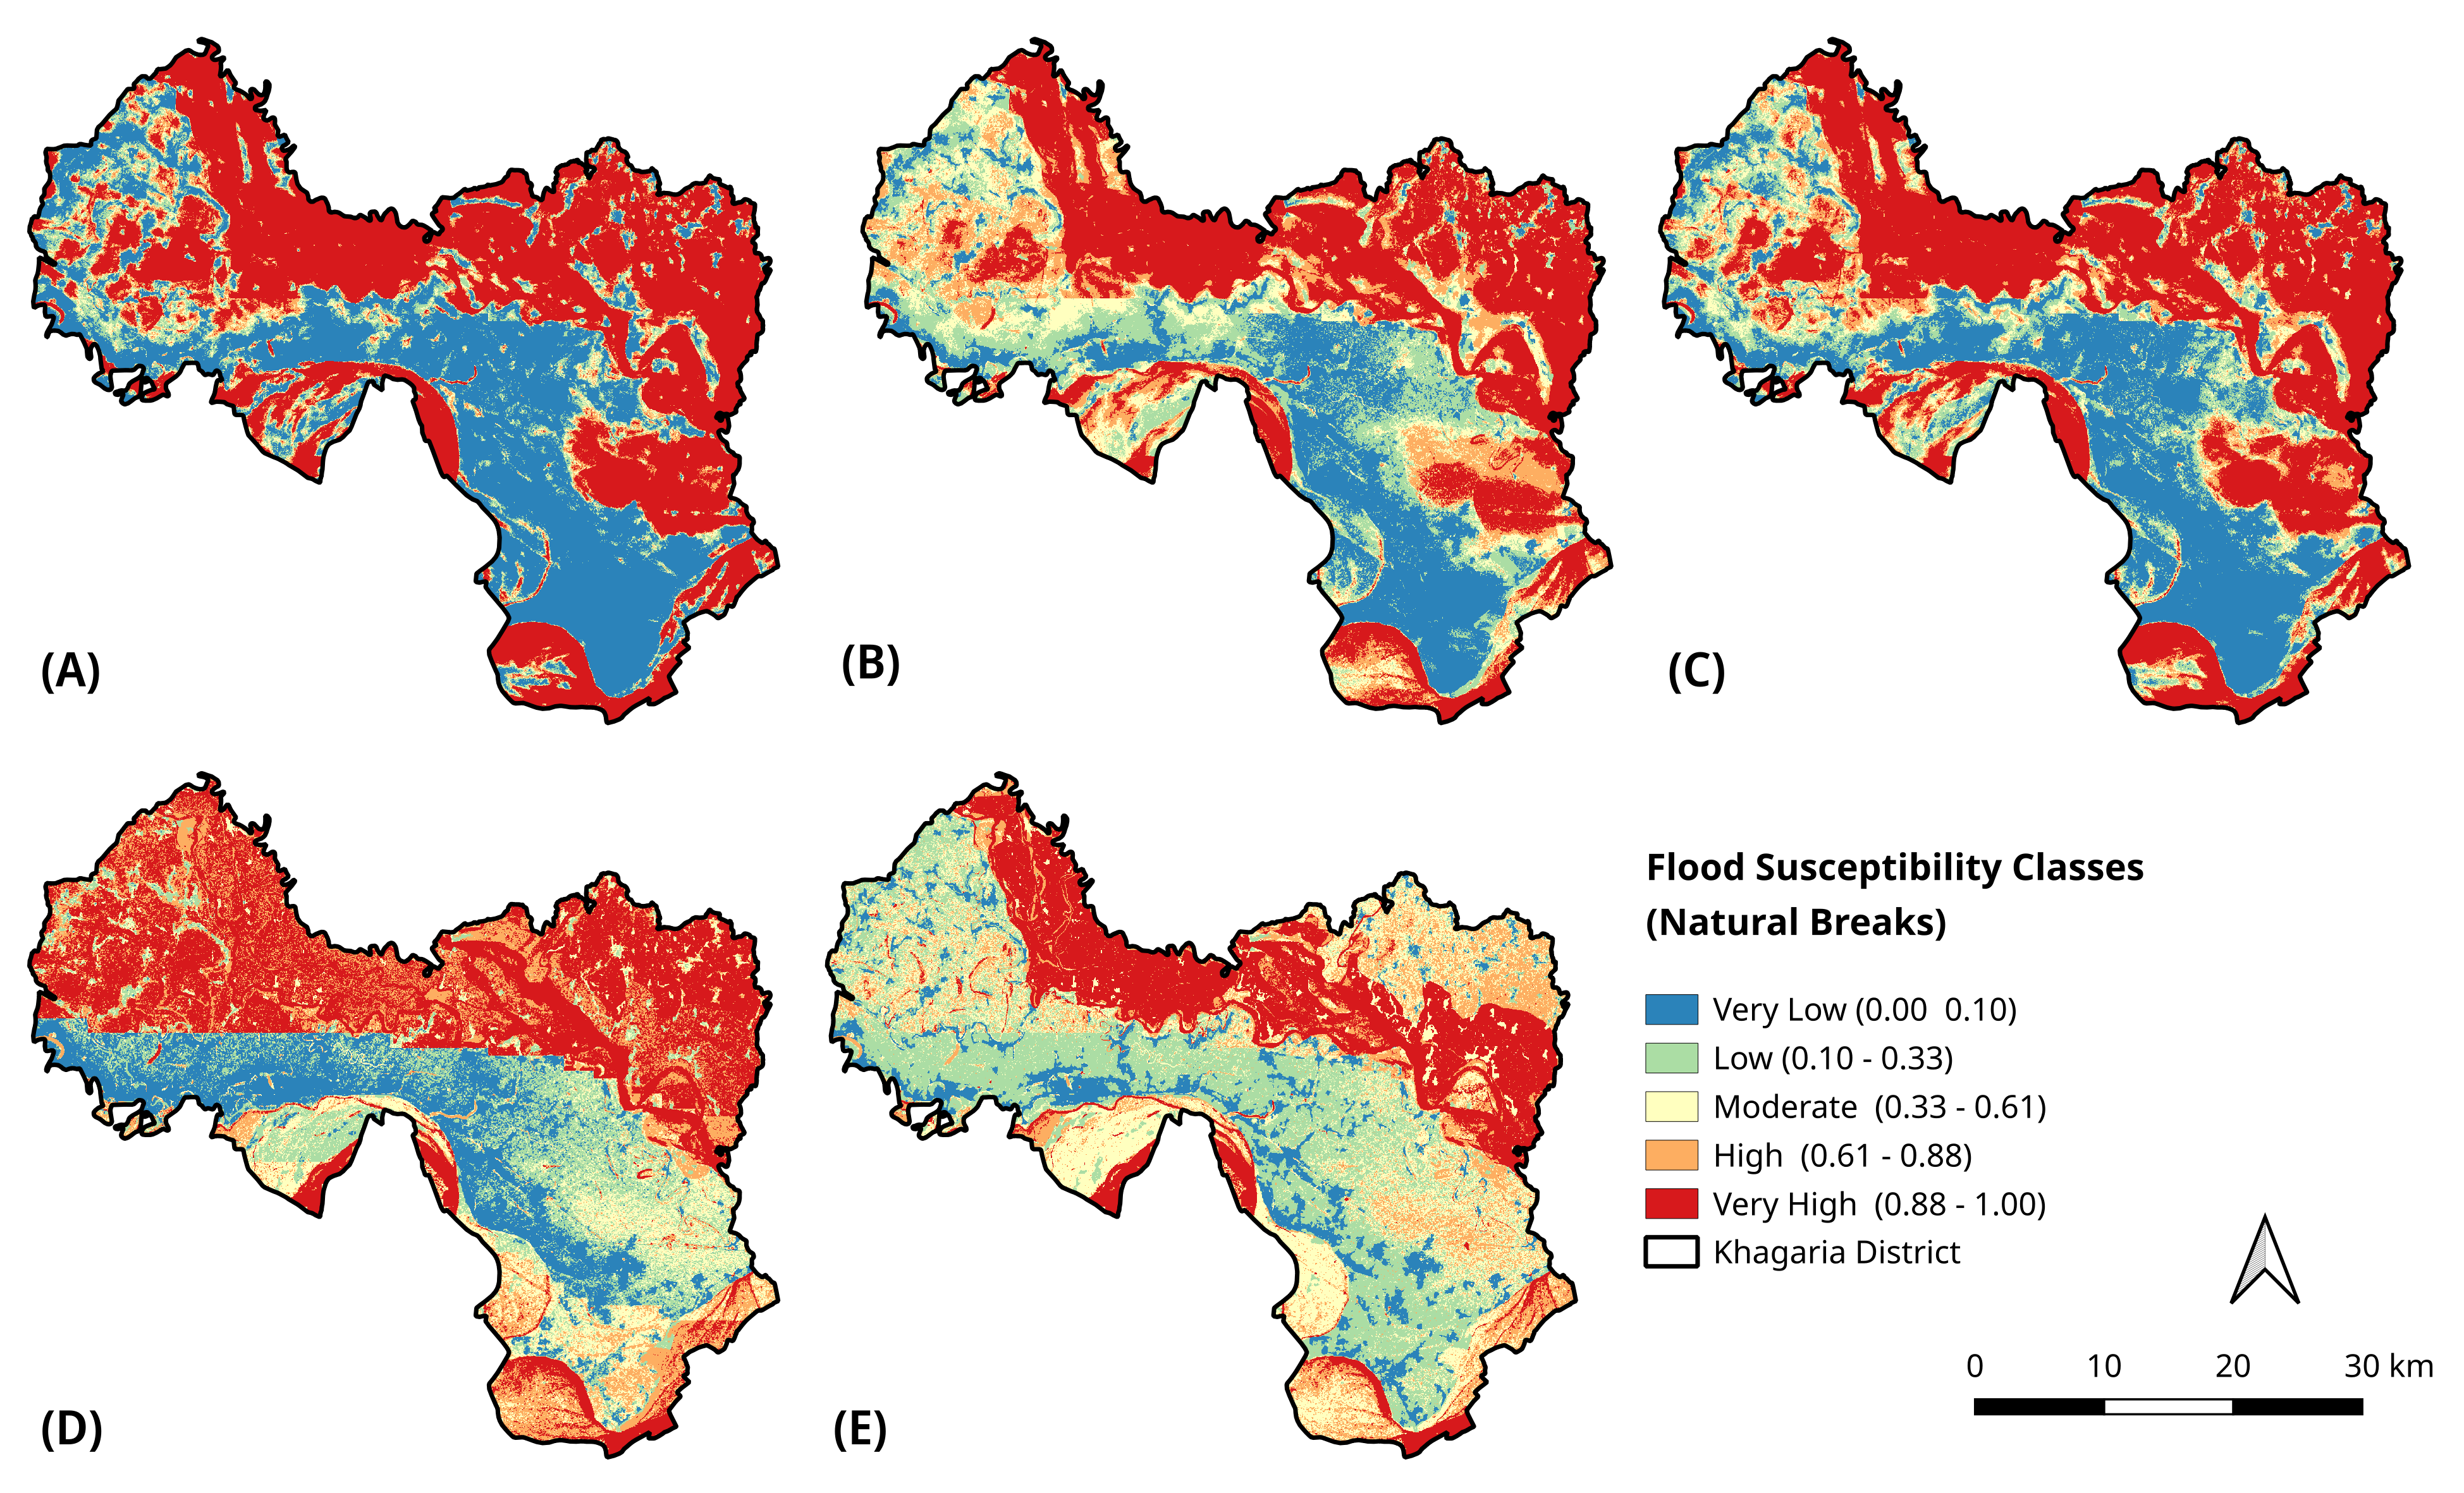
\includegraphics[width=\textwidth]{Figures/Fig_Flood_Susceptibility_Maps.png}
    \caption{Flood susceptibility probability maps (FSMs) for Khagaria district generated by all five models, classified into five natural-break susceptibility classes: Very Low (0.00--0.10), Low (0.10--0.33), Moderate (0.33--0.61), High (0.61--0.88), and Very High (0.88--1.00). (A) XGBoost; (B) CatBoost; (C) RandomForest; (D) ANN; (E) DNN. Tree-based models (A--C) produce sharper, more spatially concentrated probability transitions, particularly at river bank boundaries and elevation breaks. DNN and ANN maps (D--E) exhibit diffuse gradients with higher proportions of intermediate probability values and markedly lower Very High susceptibility zones, reflecting decision manifold uncertainty consistent with their inferior CSI.}
    \label{fig:fsm}
\end{figure}

The five FSMs show distinct spatial characteristics reflecting model architecture. XGBoost, CatBoost, and RF (Figures~\ref{fig:fsm}A--C) delineate high-susceptibility zones with sharp boundaries, concentrating Very High susceptibility in the Kosi meander belt traversing the northern district, the Burhi Gandak corridor in the western and central areas, and backwater-influenced zones in the south near the Ganga confluence. The \textit{chaur} depressions scattered throughout the mid-district appear as isolated high-susceptibility polygons sharply separated from adjacent lower-susceptibility zones, consistent with their geomorphological identity as topographic sinks. DNN and ANN (Figures~\ref{fig:fsm}D--E) produce spatially more diffuse outputs, with larger areas classified under Moderate and Low susceptibility and a substantially reduced Very High zone, indicating that smooth neural decision boundaries fail to resolve the abrupt topographic and proximity thresholds that govern alluvial inundation.

\begin{figure}[H]
    \centering
    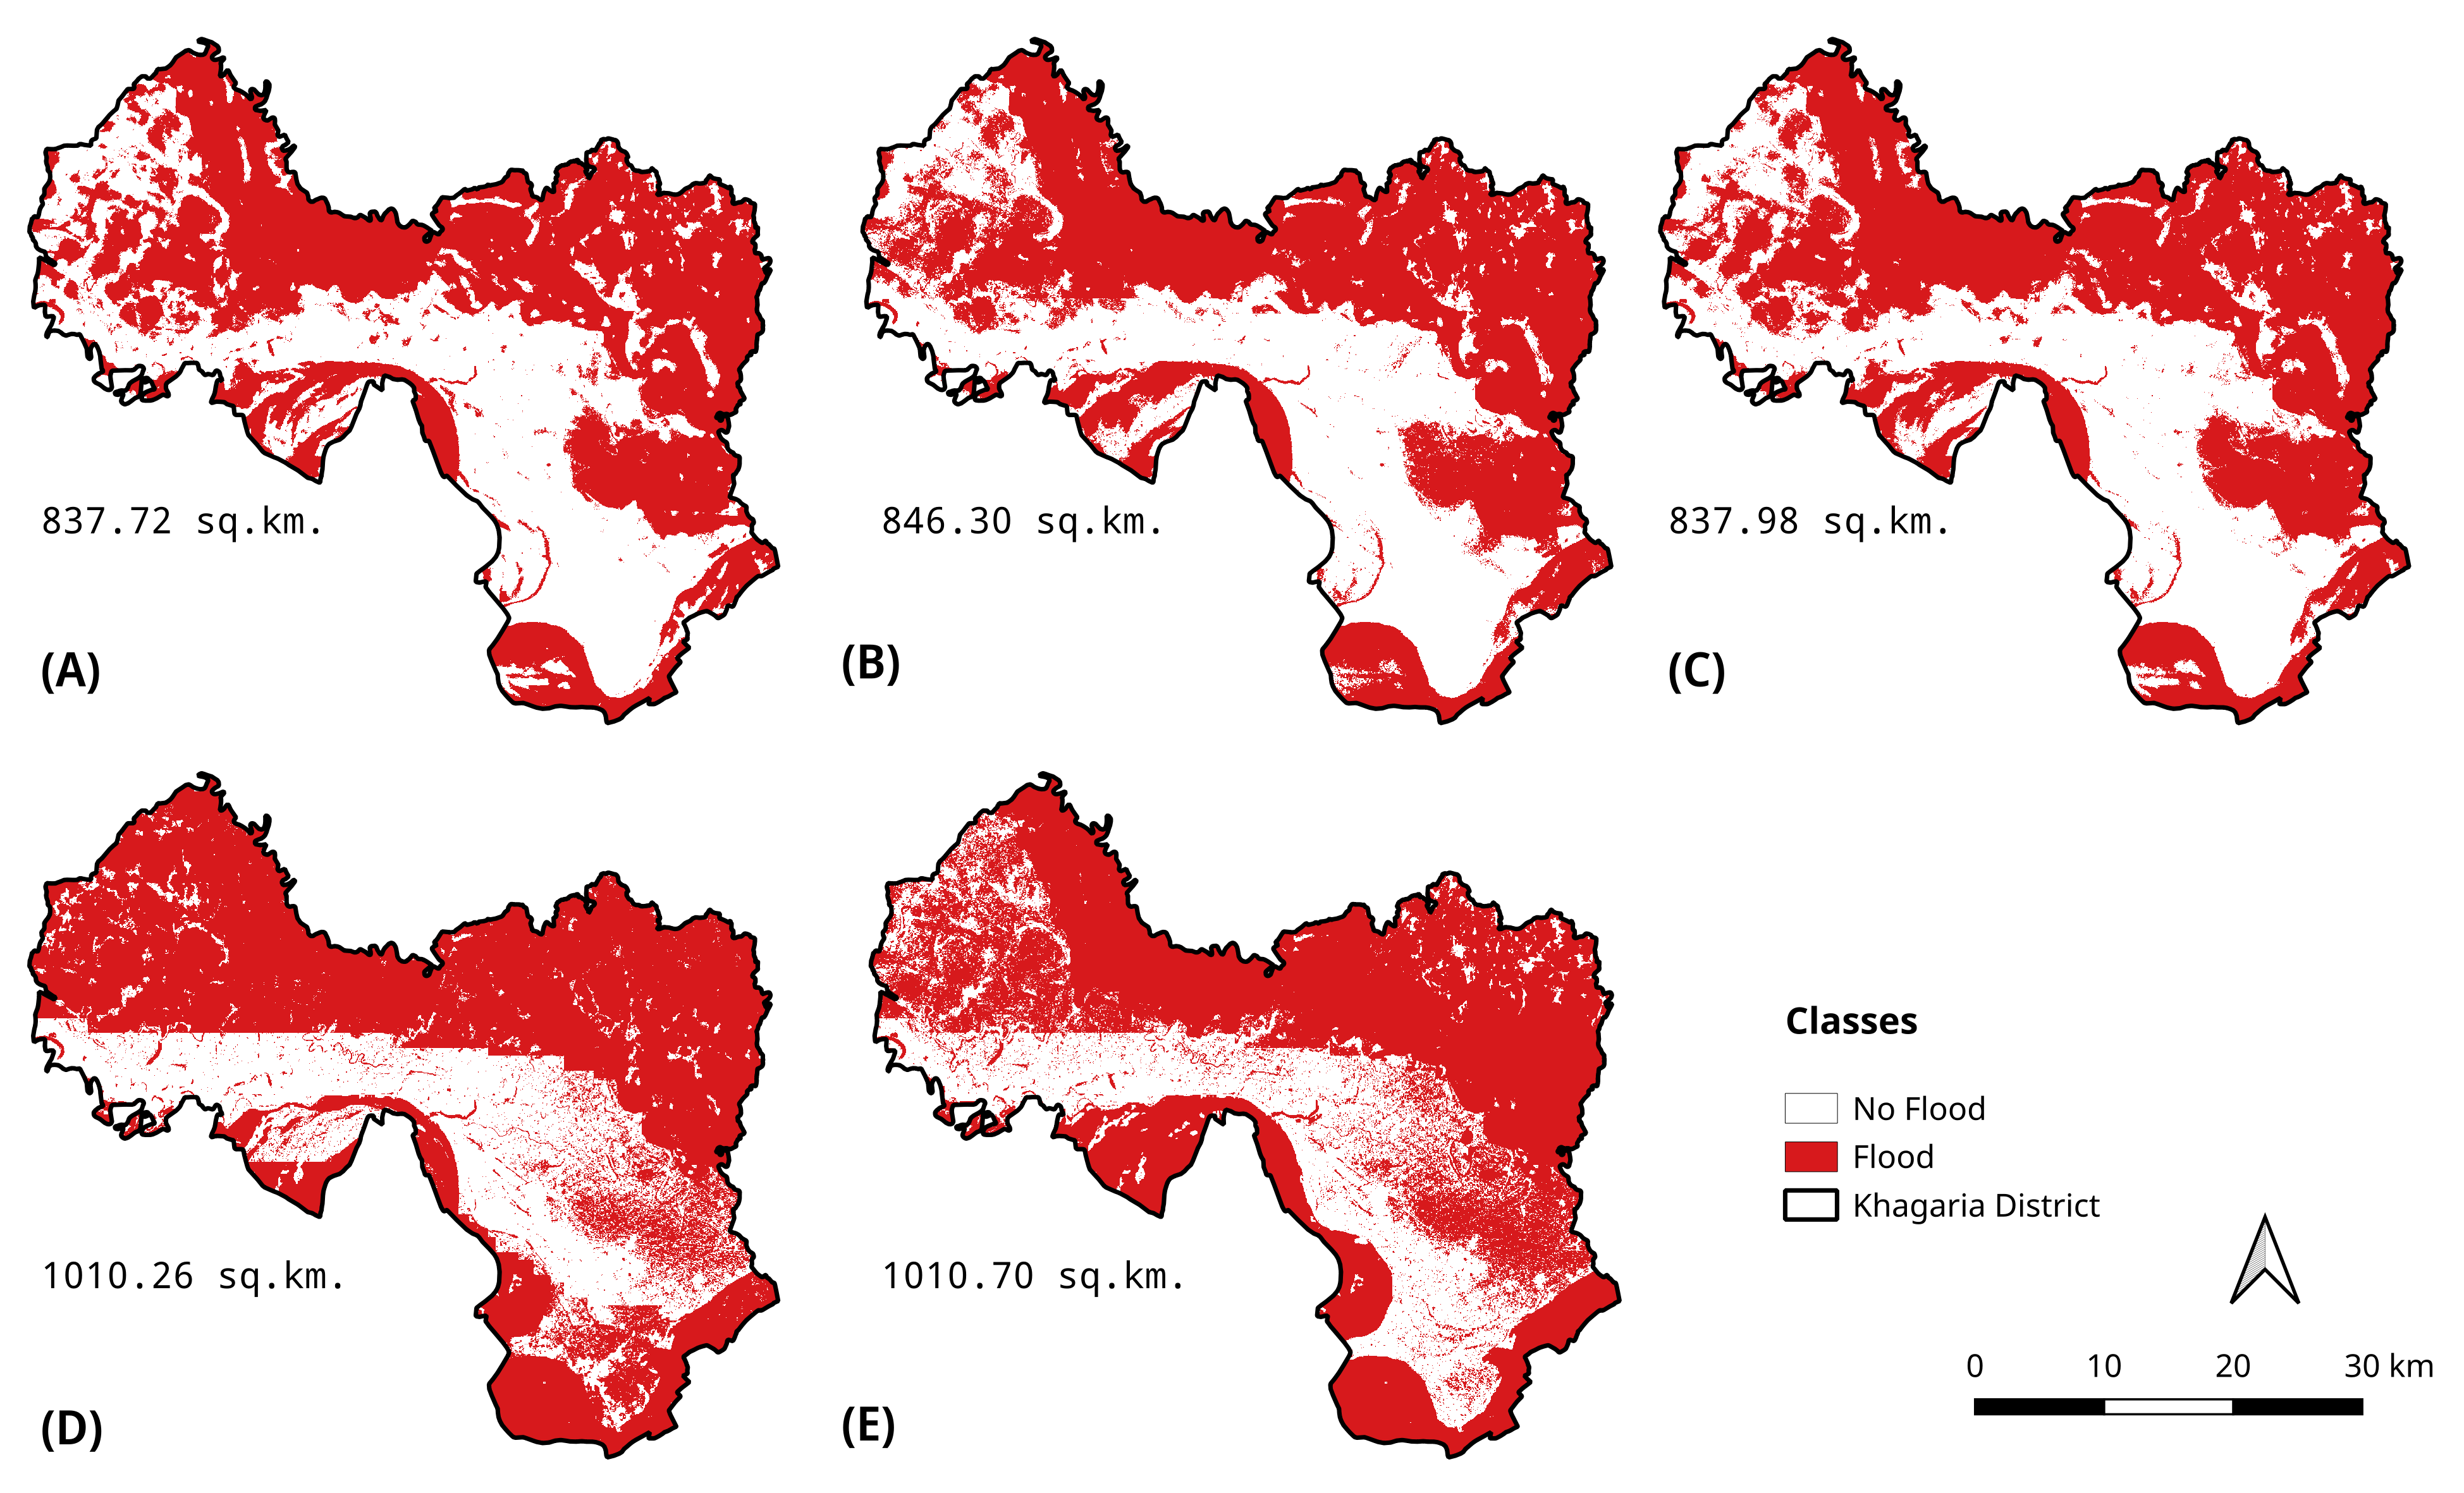
\includegraphics[width=\textwidth]{Figures/FHM.png}
    \caption{Binary flood hazard maps (FHMs) for all five models derived using Max-CSI optimal thresholds ($\tau^*$). (A) XGBoost ($\tau^* = 0.491$, flood area = 837.72 km\textsuperscript{2}); (B) CatBoost ($\tau^* = 0.500$, 846.30 km\textsuperscript{2}); (C) RandomForest ($\tau^* = 0.482$, 837.98 km\textsuperscript{2}); (D) ANN ($\tau^* = 0.372$, 1010.70 km\textsuperscript{2}); (E) DNN ($\tau^* = 0.284$, 1010.26 km\textsuperscript{2}). Red = Flood Hazard Zone; White = Safe Zone. The three tree-based models produce highly consistent flood extents (range: 837.72--846.30 km\textsuperscript{2}), closely matching the reference inventory extent of 839.40 km\textsuperscript{2}. The DL models produce substantially larger flood extents ($\approx$1,010 km\textsuperscript{2}), reflecting their lower optimal thresholds and probability miscalibration.}
    \label{fig:fhm}
\end{figure}

The derived binary FHMs (Figure~\ref{fig:fhm}) reveal a striking difference between tree-based and DL model outputs. XGBoost, CatBoost, and RF produce FHMs with total flood extents of 837.72, 846.30, and 837.98 km\textsuperscript{2} respectively --- a range of only 8.58 km\textsuperscript{2} ($< 0.6\%$ variation) and in close agreement with the reference flood inventory extent of 839.40 km\textsuperscript{2}. In contrast, DNN and ANN FHMs cover 1,010.26 and 1,010.70 km\textsuperscript{2} respectively --- an overestimate of approximately 170 km\textsuperscript{2} ($\approx$20\%) relative to the inventory. This overestimation is a direct consequence of the low optimal thresholds ($\tau^*_\text{DNN} = 0.284$; $\tau^*_\text{ANN} = 0.372$) required to maximise CSI, reflecting systematic probability compression in neural outputs.

\subsection{Susceptibility Class Area Statistics}

Table~\ref{tab:area} presents the areal distribution (as percentage of total valid district area) of each susceptibility class for all five FSMs. The XGBoost FSM assigns 22.9\% of total area to the Very High susceptibility class, compared to just 11.3\% for DNN --- reflecting the sharper delineation of extreme susceptibility zones by tree-based models. XGBoost also assigns the highest proportion to the Very Low class (67.3\%), indicating well-separated bimodal probability distributions characteristic of well-calibrated tree models. The DNN class distribution is notably flatter and more spread across intermediate classes (Low 12.7\%; Moderate 11.8\%), consistent with the diffuse probability surfaces visible in Figure~\ref{fig:fsm}.

\begin{table}[H]
\centering
\caption{Percentage area distribution of flood susceptibility classes (Natural Breaks) for each model FSM. Total valid area = 1,486 km\textsuperscript{2}.}
\label{tab:area}
\begin{adjustbox}{max width=\linewidth}
\begin{tabular}{lccccc}
\toprule
\textbf{Model} & \textbf{Very Low (\%)} & \textbf{Low (\%)} & \textbf{Moderate (\%)} & \textbf{High (\%)} & \textbf{Very High (\%)} \\
\midrule
XGBoost      & 67.26 & 4.09  & 2.45  & 3.29  & 22.90 \\
CatBoost     & 64.16 & 5.98  & 4.33  & 5.34  & 20.19 \\
RandomForest & 60.75 & 8.27  & 6.28  & 7.36  & 17.34 \\
ANN          & 59.06 & 7.41  & 6.33  & 9.42  & 17.79 \\
DNN          & 55.71 & 12.71 & 11.78 & 8.50  & 11.31 \\
\bottomrule
\end{tabular}
\end{adjustbox}
\end{table}

%% ============================================================
%%  5. DISCUSSION
%% ============================================================
\section{Discussion}

\subsection{Physical Interpretation of SHAP-Derived Feature Importance}
\label{sec:disc_shap}

The SHAP analysis provides a physically grounded and model-conditioned explanation for \textit{why} tree-based models outperform DL in this domain.  The top four predictors --- Geomorphology, Soil, Rainfall, and Elevation --- collectively account for the primary axes of alluvial flood susceptibility in Khagaria, and their cross-model consistency validates that the trained models have captured genuine hydro-geomorphic process relationships rather than spurious statistical correlations.

\paragraph{Geomorphology as the dominant integrative predictor.}
Geomorphology's unit-normalised SHAP score (1.000) under XGBoost reflects its unique role as an integrated, process-aware landform classifier that encodes causal information unavailable to any single topometric index.  The XGBoost beeswarm plot (Figure~\ref{fig:shap_beeswarm_xgb}) shows that \textit{chaur}-class pixels (higher Geomorphology class values) consistently receive strongly positive SHAP contributions, directly mapping to Khagaria's topographic sinks that trap monsoon and backwater inundation.  Natural levees and older alluvial terraces receive near-zero or negative SHAP contributions from Geomorphology.  This finding is broadly consistent with the geomorphic flood index framework of \citet{samela2017} and the geomorphological conditioning evidence in the Bihar flood literature \citep{sinha2008}, confirming that landform classification subsumes much of the predictive content of terrain derivatives in near-flat alluvial environments.

\paragraph{Soil type: the infiltration--runoff switch.}
Soil Type's second-rank SHAP position (0.867) is physically explained by the soil's role as the primary threshold between infiltration-dominated and runoff-dominated response.  In the Khagaria context, fine-textured alluvial clays on the floodplain surface rapidly reach field capacity and then generate direct surface runoff, while sandy loam soils on levee crests and \textit{diara} land maintain higher infiltration capacities throughout the monsoon season \citep{NBSSLUPbihar2020}.  The SHAP beeswarm shows that clay-dominant soil pixels (high feature value, red) receive strongly positive flood probability contributions, while sandy-loam pixels (low feature value, blue) receive negative contributions.

\paragraph{Rainfall and the meteorological trigger.}
Rainfall's third-rank SHAP score (0.783) confirms its role as the primary triggering forcing while also revealing a methodologically important distinction from gain-based importance (GAIN rank = 0.275).  The divergence arises from the difference between \textit{global split utility} (GAIN: does this feature appear early in the tree structure?) and \textit{conditional marginal contribution} (SHAP: how much does this feature change predictions once Geomorphology and Soil are already conditioned on?).  Rainfall's lower GAIN reflects that it appears deeper in the XGBoost trees --- after Geomorphology and Soil have already segregated the major risk classes --- but its high SHAP score confirms substantial residual predictive information.  This distinction matters operationally: gain-based rankings used without SHAP verification can systematically underweight meteorological drivers in alluvial flood models, leading to under-investment in rainfall monitoring as a flood early-warning input.

\paragraph{Model-specificity of importance profiles.}
The cross-model rank heatmap (Figure~\ref{fig:shap_heatmap}) reveals that while the top-four predictors are shared across tree models, CatBoost elevates Rainfall to rank 1 and Dist.\ to Roads to rank 2 relative to XGBoost, reflecting the Ordered Boosting algorithm's different split utility formulation.  ANN and DNN importance profiles are more diffuse (lower peak SHAP values, flatter importance curves), consistent with smooth neural decision manifolds distributing prediction responsibility across many features simultaneously rather than concentrating it in sharp axis-aligned splits.  This distributional difference further explains DL's inferior CSI: when decision boundaries are smooth and importance is distributed, the model cannot replicate the step-wise threshold logic of alluvial flood inundation.

\paragraph{Curvature and TWI: null importance in flat terrain.}
Curvature's SHAP score of exactly 0.000 and Aspect's near-zero score (0.035) confirm empirically that these terrain derivatives carry no residual predictive information beyond what Geomorphology, Elevation, Soil, and Rainfall already provide in this near-flat domain.  This finding has a direct practical implication: flood susceptibility studies that routinely include all SRTM-derived terrain indices without importance validation risk adding noise predictors that inflate model complexity without improving operational performance \citep{tehrany2019, khosravi2018}. TWI's low SHAP score (0.082) in this domain is physically consistent: the TWI formulation \mbox{($\text{TWI} = \ln(A_s/\tan\beta)$)} becomes numerically unstable in near-zero-slope terrain, producing extreme values that carry no reliable gradient information. Excluding TWI and Slope from DL models is therefore not merely a collinearity necessity but also an importance-aligned choice.

\subsection{Why Tree-Based Models Outperform Deep Learning on Tabular Geospatial Data}

The results provide rigorous empirical support for the Tabular Data Hypothesis \citep{grinsztajn2022, shwartzziv2022, mcelfresh2023}: gradient-boosted decision trees decisively outperform neural architectures on structured, medium-scale tabular datasets. The CSI gap between XGBoost (0.937) and the best DL model, DNN (0.705), is 0.232 points --- operationally consequential in a flood hazard context where decisions directly govern life safety and infrastructure investment.

The most fundamental explanation is inductive bias \citep{Mitchell1980}. Flood susceptibility in alluvial plains is physically governed by threshold-type, orthogonal decision rules: a pixel is at risk if Elevation is below a critical value, AND Distance to River is within a proximity threshold, AND local drainage is constrained by low Slope and high TWI. These axis-aligned conditions are precisely what recursive binary partitioning in decision trees is designed to represent \citep{breiman2001}. Neural networks, applying stacked linear transformations with smooth activations, impose a prior favouring smooth, continuous decision manifolds --- a prior structurally mismatched to the step-wise physical logic of alluvial flood inundation \citep{Popov2021}. This mismatch leads to the diffuse, poorly calibrated probability surfaces in the ANN and DNN FSMs (Figure~\ref{fig:fsm}D--E), and to their anomalously low optimal thresholds ($\tau^*_\text{DNN} = 0.284$; $\tau^*_\text{ANN} = 0.372$) indicating systematic probability compression \citep{Niculescu-Mizil2005, zadrozny2002}. The consequence is operationally severe: applying a standard 0.5 threshold to the DNN output would miss the 170 km\textsuperscript{2} overestimated by the DL FHM, and applying the correct $\tau^* = 0.284$ produces geographically expanded hazard zones that over-designate safe areas.

Where DL does excel in hydrology is in tasks with fundamentally different structural properties. Long Short-Term Memory networks and Transformer architectures applied to time-series streamflow forecasting \citep{Kratzert2018, Frame2022} leverage temporal autocorrelation and sequential process dynamics across thousands of basin-hours of training data. Large-scale weather prediction models \citep{Bi2023, Lam2023} exploit the high spatial dimensionality of gridded atmospheric fields with billions of training examples. In these contexts, the hierarchical feature extraction capability of DL adds genuine value that tabular tree models cannot replicate. The key discriminating factor is data structure and scale: DL is the appropriate choice when inputs are high-dimensional (images, time series, gridded fields), spatially or temporally structured, and abundant; tree ensembles are the more reliable default for structured tabular classification with a finite set of handcrafted features and hundreds of thousands to a few million training samples \citep{mcelfresh2023, shwartzziv2022}. For flood susceptibility mapping specifically, where each pixel is described by 10--20 terrain-derived attributes computed from SRTM, SAR, and land-cover products, the data structure firmly falls in the latter category.

Data scale compounds this architectural mismatch. DL's competitive advantage manifests most powerfully with very large, highly varied training corpora \citep{lecun2015, Vaswani2017}. District-level geospatial inventories --- even at 30 m resolution across 1,486 km\textsuperscript{2} --- yield a training set of hundreds of thousands of pixels described by 12--14 features, far below the scale at which DL achieves consistent advantages over tree ensembles \citep{shwartzziv2022}. Dropout and batch normalisation partially mitigate overfitting, but ensemble methods achieve more efficient implicit regularisation through bootstrap sampling and random feature subsampling \citep{dietterich2000, breiman2001}. Feature robustness adds a third layer: XGBoost and CatBoost retained the perfectly collinear Slope and TWI features without performance degradation, while neural networks required their exclusion to train stably --- a direct consequence of gradient-based optimisation being destabilised by collinear inputs. These findings reinforce recent geohazard-specific evidence: \citet{Arabameri2021} found XGBoost superior to ANN in gully erosion susceptibility; \citet{Iban2022} reported CatBoost outperforming DL for landslide susceptibility; \citet{zhang2022} demonstrated XGBoost dominance in multi-hazard susceptibility frameworks; and \citet{Arora2024Argens} showed that RF and XGBoost outperformed ANN when benchmarked against high-resolution hydrodynamic flood hazard maps over the Argens Basin, France. The implication for practitioners is clear: unless the input data includes image patches, time series, or other structured non-tabular features, tree-based ensembles should be the default first choice for geospatial hazard susceptibility mapping with conventional CgF inputs.

\subsection{Max-CSI Thresholding and Operational Hazard Map Quality}

The consistent Max-CSI superiority over Youden's Index (mean $\Delta\text{CSI} = +0.013$) and the fixed 0.5 threshold extends beyond this study to the broader flood hazard mapping literature, where most published works adopt default thresholding without accounting for the operational consequences of false negatives \citep{tehrany2019, Costache2020, Arora2022SERRA}. In flood hazard zonation, the cost asymmetry is clear: missed flood zones contribute directly to underprotection of lives, property, and infrastructure; unnecessary hazard designations impose economic costs of land-use restrictions and emergency preparedness. The CSI, by penalising TP, FP, and FN simultaneously, is uniquely aligned with this objective \citep{schaefer1990, mason2003}. The 2.0 percentage-point CSI improvement of Max-CSI over the fixed 0.5 threshold in XGBoost translates, at 30 m resolution across 1,486 km\textsuperscript{2}, to thousands of hectares correctly reclassified --- areas with direct consequences for DDMA land-use planning and infrastructure investment.

The close agreement between XGBoost FHM extent (837.72 km\textsuperscript{2}) and the reference SAR-derived inventory (839.40 km\textsuperscript{2}) is particularly noteworthy. This close correspondence --- a difference of only 1.68 km\textsuperscript{2} ($< 0.2\%$) --- should nevertheless be interpreted with care: because maximising the CSI drives false-positive and false-negative counts towards balance, CSI-optimal thresholding mathematically pulls predicted flood area towards the reference area, so extent agreement is partly a property of the criterion rather than fully independent validation. The informative contrast is that the DL models fail to achieve this correspondence even at their CSI-optimal thresholds --- overestimating extent by $\approx$170 km\textsuperscript{2} --- demonstrating that threshold optimisation cannot compensate for a miscalibrated probability surface. CatBoost and RF FHMs also show close correspondence (846.30 and 837.98 km\textsuperscript{2} respectively), underscoring the robustness of tree-based models for binary hazard delineation. The anomalously low optimal thresholds for DNN and ANN further highlight that DL models produce poorly calibrated probability outputs even when AUC is competitive. Probability calibration methods --- Platt scaling \citep{platt1999}, isotonic regression, or temperature scaling --- should be considered necessary post-processing steps before DL-based susceptibility maps are used operationally.

\subsection{Bihar Floods and the Upper North Bihar Crisis Zone}

The derived XGBoost FHM spatially resolves flood dynamics that are qualitatively well-understood in the Bihar flood literature but have not previously been mapped at pixel-level resolution using ML methods. High-hazard zones trace the Kosi meander belt, the Burhi Gandak corridor, and the Ganga backwater zone with precision that closely mirrors historical flood damage records \citep{bhuvan2010, tatatrusts2024, sinha2008, Arora2025SciRep, Arora2022SERRA}. The model's delineation of \textit{chaur} depressions as distinct high-hazard polygons sharply separated from safer levee ridges resolves sub-kilometre geomorphological features operationally critical for waterlogging risk assessment but absent from coarser official flood atlases \citep{bhuvan2010}.

The upper North Bihar region --- spanning the Himalayan foothills and the immediate flood-receiving districts of Darbhanga, Sitamarhi, Madhubani, Supaul, and Saharsa in addition to Khagaria --- constitutes one of the most consistently and severely flood-affected corridors on Earth. The driving mechanism is structurally embedded: the Kosi, Bagmati, Gandak, and Kamla Balan all originate in Nepal's Himalayas, where snowmelt and concentrated monsoon precipitation generate simultaneous peak discharges that arrive on the Bihar plains within days of each other \citep{sinha2008, mishra2018, Jha2012, Costache2021Geocarto}. The Kosi's extraordinary sedimentation rate --- approximately 100--150 million tonnes annually \citep{sinha2008} --- has progressively raised its bed above the surrounding floodplain, making it a perched, above-grade river structurally prone to avulsion. The 2008 Kusaha breach, in which the Kosi shifted its course by approximately 120 km in days and inundated over 3,400 km\textsuperscript{2} of Bihar, is the most extreme recent manifestation of this dynamic \citep{bhuvan2010, mishra2018}. The embankment system constructed since the 1950s has, paradoxically, accelerated bed aggradation within embankments and transferred catastrophic breach risk to downstream districts like Khagaria \citep{beams2024, mishra2018}. ML susceptibility studies of the type conducted here --- operating at pixel level with multi-year SAR-calibrated inventories --- are uniquely positioned to resolve the spatial heterogeneity of this hazard within individual districts. Identification of specific blocks (Parbatta, Gogri, Alauli, Beldaur, Mansi) and landscape elements (\textit{chaurs}, river confluence zones, backwater-prone areas) as consistently high-hazard provides the DDMA with spatial precision needed for targeted embankment reinforcement, early warning system placement, and pre-monsoon evacuation planning. Extension of this methodology to the full upper North Bihar crisis zone --- integrating dynamic variables such as Kosi discharge at Bhimnagar barrage, Sentinel-1-derived soil moisture, and SWOT water surface elevations \citep{Biancamaria2016} --- represents a tractable and high-impact direction for future operational flood forecasting in one of the world's most vulnerable river systems.

\subsection{Spatial Implications and Comparison with Official Assessments}

The pixel-level hazard resolution of the XGBoost FHM represents a material improvement over existing official flood hazard atlases \citep{bhuvan2010} that classify hazard at block level. The XGBoost map delineates intra-block heterogeneity at 30 m --- identifying elevated levee ridges along the Kosi and Burhi Gandak as locally safe corridors within otherwise high-hazard blocks, and distinguishing the variable susceptibility of the Parbatta block (where Kosi and Kareh channels produce contrasting micro-topographic flood exposure) from the uniformly high-hazard character of Mansi and Alauli blocks at the Ganga confluence. This spatial detail is operationally critical for siting flood shelters, planning evacuation routes, and prioritising infrastructure protection. The consistency of XGBoost, CatBoost, and RF flood extents (837.72--846.30 km\textsuperscript{2}) further reinforces confidence in the hazard delineation: despite using different algorithmic approaches, all three converge on $\approx 56\%$ of district area as flood-susceptible, consistent with Bihar's district-level historical vulnerability statistics \citep{beams2024}.

The well-calibrated $\tau^* = 0.491$ for XGBoost --- marginally below 0.5 --- confirms that the model's probability surface faithfully represents flood risk. By contrast, the DNN's $\tau^* = 0.284$ implies that a conventional 0.5 threshold would misclassify a substantial fraction of high-risk pixels as safe, with potentially severe consequences in an operational context. This calibration disparity is a strong empirical argument for mandatory threshold validation as part of any flood susceptibility study intended for operational deployment.

\subsection{Limitations and Future Directions}

Several limitations merit acknowledgement. First, and most importantly from a validation standpoint, the 80:20 partition used stratified \textit{random pixel-level} sampling. Because conditioning factors are strongly spatially autocorrelated at 30 m resolution, test pixels frequently neighbour training pixels in both geographic and feature space; the reported accuracy metrics --- including the near-perfect tree-ensemble AUC --- therefore measure \textit{interpolative} skill within the sampled domain and are likely optimistic with respect to transferability to unseen regions or events \citep{roberts2017, ploton2020}. Spatially blocked cross-validation, in which entire contiguous zones are withheld, is the appropriate protocol for estimating extrapolative performance and constitutes a priority for follow-up work. Importantly, this inflation affects all five models symmetrically and therefore does not alter the comparative conclusions or the relative merit of the Max-CSI framework, both of which are within-design contrasts. Second, the equal-effort configuration protocol means the neural architectures were not exhaustively tuned; deeper hyperparameter search (learning-rate schedules, early stopping, architecture search) could narrow the observed gap, although tabular benchmarks indicate that tuned deep models rarely overtake tuned gradient-boosted trees at this data scale \citep{grinsztajn2022, shwartzziv2022, mcelfresh2023}. Third, the study relies on 30 m SRTM elevation data, which cannot resolve micro-topographic features --- irrigation canal embankments, road beds, settlement mounds --- that locally modulate inundation at sub-50 m scales \citep{neal2021, Hawker2022}. Integration of LiDAR or Cartosat-3 DEM would substantially enhance spatial precision, particularly for \textit{diara} ridge delineation and road-bounded drainage compartments. The flood inventory, although multi-year (2008, 2020, 2021), does not yet incorporate the 1987, 2004, and 2024 events; a full multi-decadal inventory would enable the model to learn the complete envelope of Khagaria's flood frequency distribution. The static CgF-based model treats terrain as fixed, precluding direct application to event-specific forecasting where antecedent soil moisture, real-time discharge, and embankment integrity dominate \citep{sinha2008, mishra2018}. Future work should integrate near-real-time hydrological variables --- CWC gauge data, SWOT water surface elevations \citep{Biancamaria2016}, and Sentinel-1 soil moisture --- within an XGBoost or CatBoost framework for dynamic, event-specific flood probability maps. A particularly promising direction to overcome the current data limitation is the use of hydraulic model outputs as the training target. A two-dimensional hydrodynamic simulation (e.g., HEC-RAS 2D, LISFLOOD-FP, or ANUGA) calibrated to the Kosi--Ganga system and run for standard return-period scenarios --- 100-year, 500-year, and 1,000-year recurrence intervals --- would provide physically rigorous, probabilistically interpreted inundation extents as target rasters \citep{teng2017, Bates2010}. Training an XGBoost or CatBoost model on these synthetic hydraulic targets would enable the ML framework to implicitly learn extreme-event flood dynamics that have not yet been observed in the multi-event SAR inventory, effectively extending the training envelope to rare but operationally critical scenarios. This hydraulic-ML hybrid approach bridges the data-scarcity limitation inherent to historical SAR inventories and aligns ML susceptibility products with the return-period framework already used by engineers and planners for infrastructure design \citep{neal2021, teng2017}.

Additional directions include LightGBM \citep{ke2017} as a complementary tree-based competitor, post-hoc probability calibration for DL models, and Transformer-based tabular architectures \citep{Gorishniy2021} as the DL frontier evolves.

%% ============================================================
%%  6. CONCLUSION
%% ============================================================
\section{Conclusion}

This study presented a rigorous multi-model comparative analysis of ML and DL approaches for flood susceptibility mapping and FHM derivation in Khagaria district, Bihar --- one of India's most persistently flood-affected districts, situated at the convergence of seven major Himalayan and peninsular river systems. A multi-year multi-mission SAR flood inventory --- ENVISAT ASAR (2008) and Sentinel-1 (2020, 2021) --- integrating 839.40 km\textsuperscript{2} of reference flood extent was combined with fourteen geo-environmental conditioning factors and processed through a Hybrid Prediction Pipeline separating tree-based and DL model branches based on VIF-based collinearity screening.

XGBoost achieved the highest performance across all validation metrics (AUC = 0.9982; CSI = 0.9372; Sensitivity = 0.9666; Specificity = 0.9882; $\tau^* = 0.491$), followed by CatBoost (AUC = 0.9935; CSI = 0.8711) and RF (AUC = 0.9910; CSI = 0.8444), while DNN and ANN yielded substantially lower CSI values of 0.705 and 0.668 respectively, confirming the Tabular Data Hypothesis within the flood susceptibility domain. The performance advantage of tree-based models is mechanistically rooted in their inductive bias for the axis-aligned, threshold-type decision boundaries that physically govern alluvial flood inundation, their robustness to collinear features including the infinite-VIF Slope--TWI pair identified in near-flat alluvial terrain, and their efficiency at implicit regularisation on district-scale training inventories. The anomalously low optimal thresholds for DNN ($\tau^* = 0.284$) and ANN ($\tau^* = 0.372$) reveal systematic probability miscalibration that substantially limits operational utility without post-hoc calibration.

Max-CSI threshold optimisation produced binary FHMs with consistently higher CSI than Youden's Index (mean $\Delta\text{CSI} = +0.013$), with the XGBoost FHM at $\tau^* = 0.491$ yielding a flood extent of 837.72 km\textsuperscript{2} that closely matches the SAR-derived inventory (839.40 km\textsuperscript{2}). The derived FHM resolves intra-district flood heterogeneity at 30 m resolution --- identifying the Kosi meander belt, Burhi Gandak corridor, Ganga backwater zone, and \textit{chaur} depressions as high-hazard zones consistent with historical flood records --- and represents a substantially finer spatial product than existing block-level official assessments. The XGBoost FSM assigns 22.9\% of Khagaria's area to Very High susceptibility and 56.4\% to flood hazard, providing the DDMA with actionable spatial targeting for embankment reinforcement, shelter siting, and evacuation planning.

Future priorities include dynamic integration of real-time hydrological variables for event-specific forecasting, incorporation of higher-resolution elevation data (LiDAR/Cartosat-3), extension of the multi-year inventory to include the 1987, 2004, and 2024 floods, application of probability calibration techniques to DL-based susceptibility outputs before operational deployment, and scaling the methodology to the full upper North Bihar crisis zone for comprehensive district-level flood risk governance.

%% ============================================================
%%  DECLARATIONS
%% ============================================================

\section*{Statements and Declarations}

%
%
%
\subsection*{Funding}
The first author is supported by the Marie Sk\l odowska-Curie COFUND Fellowship through the SMASH programme, co-funded by the European Union's Horizon Europe Research and Innovation Programme under Grant Agreement No.\ 101081355. The funder had no role in study design, data collection and analysis, decision to publish, or preparation of the manuscript.

\subsection*{Competing Interests}
The authors declare that they have no competing financial interests or personal relationships that could have influenced the work reported in this paper.

\subsection*{Data Availability}
The flood inventory raster, CgF datasets, trained model files, and Python analysis scripts are available from the corresponding author upon reasonable request. Sentinel-1 SAR imagery is publicly available through the Copernicus Open Access Hub (\url{https://scihub.copernicus.eu}).

\subsection*{Ethics Approval}
Not applicable. This study did not involve human participants or animals.

\section*{Acknowledgements}
The first author is supported by the Marie Sklodowska-Curie COFUND Fellowship through the SMASH programme (European Union's Horizon Europe Research and Innovation Programme, Grant Agreement No. 101081355) at the University of Nova Gorica, hosted at the Slovenian Environment Agency (ARSO). The authors acknowledge the
Flood Management Information System Centre (FMISC), Water Resources Department, Government of Bihar, for providing district-level hydrological baseline data. Sentinel-1 data were obtained from the European Space Agency Copernicus Programme free of charge.

%% ============================================================
%%  REFERENCES
%% ============================================================
\newpage
\bibliographystyle{abbrvnat}
\bibliography{references}



%% ============================================================
%%  SUPPLEMENTARY MATERIAL
%% ============================================================
\newpage
\section*{Supplementary Material}

\setcounter{figure}{0}
\renewcommand{\thefigure}{S\arabic{figure}}
\setcounter{table}{0}
\renewcommand{\thetable}{S\arabic{table}}

\begin{figure}[H]
  \centering
  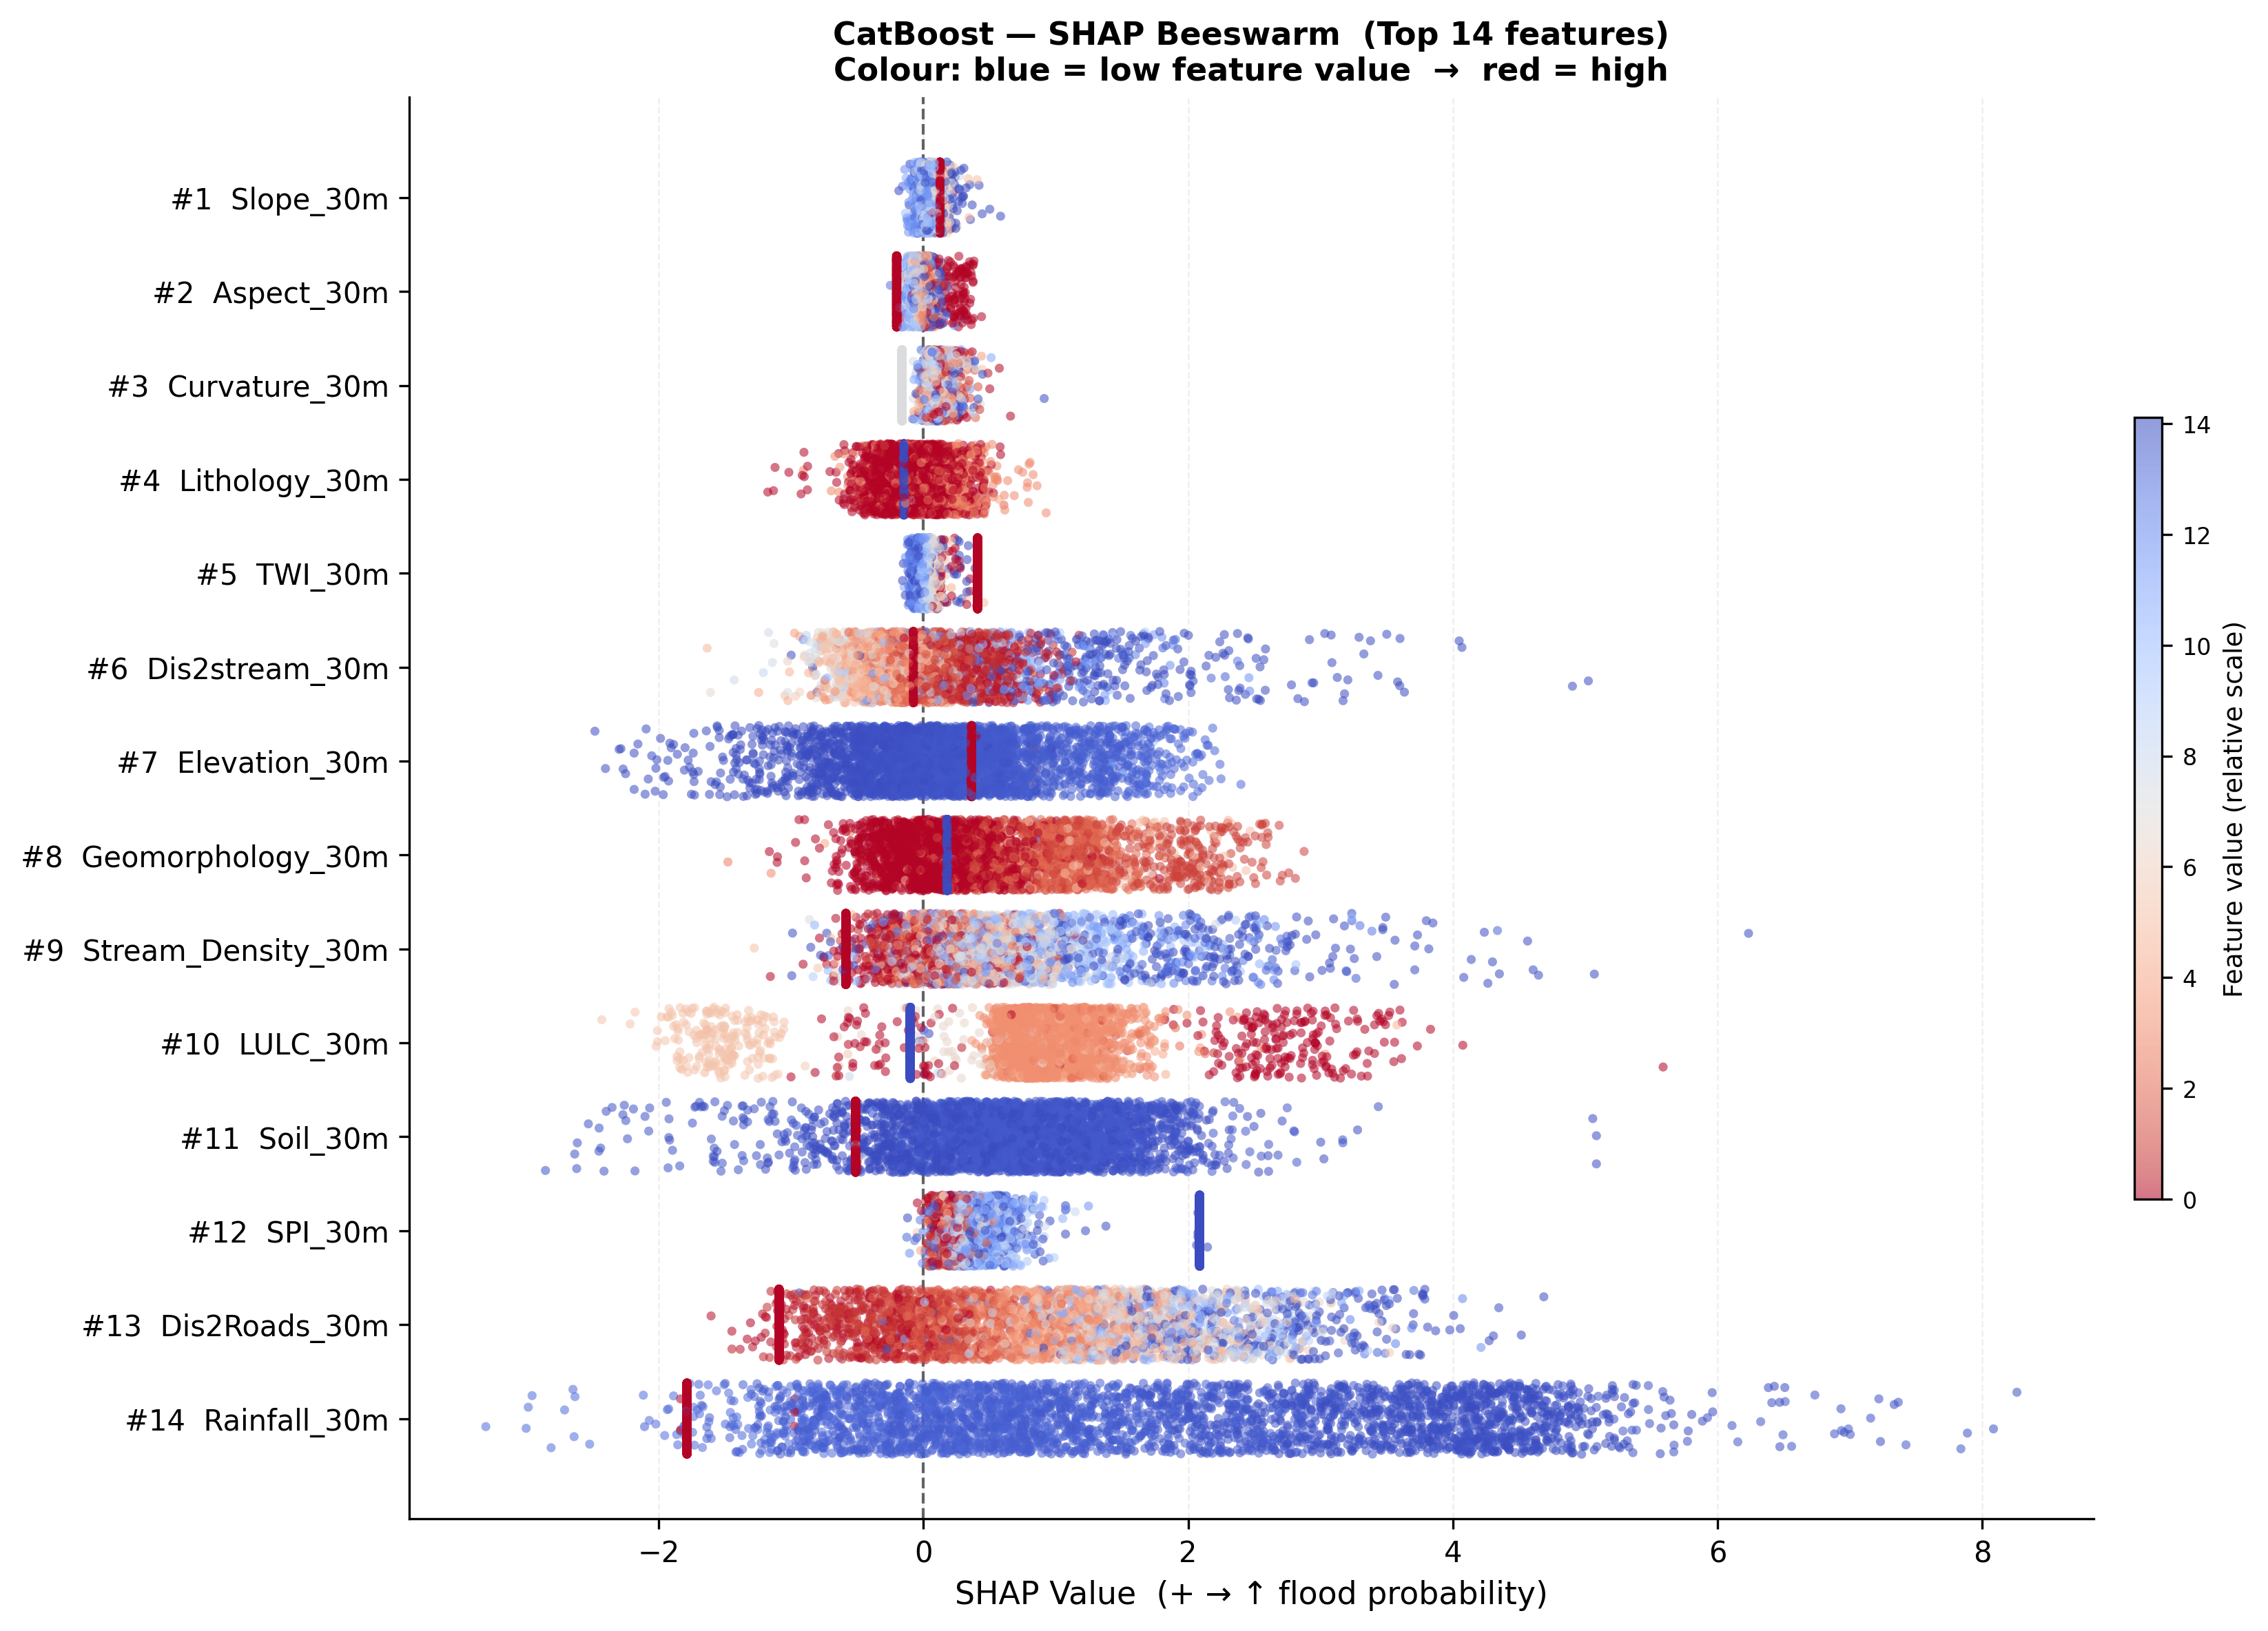
\includegraphics[width=\textwidth]{Figures/Fig_SHAP_Beeswarm_CatBoost.png}
  \caption{CatBoost SHAP beeswarm plot (top 13 features). Rainfall ranks first for CatBoost, reflecting the ordered-boosting algorithm's sensitivity to the primary meteorological trigger. Dist.\ to Roads ranks second, capturing road embankment effects on local drainage.  Compare with XGBoost beeswarm (Figure~\ref{fig:shap_beeswarm_xgb}): the top-four set \{Geomorphology, Soil, Rainfall, Elevation\} is common to both models, though rank order differs.}
  \label{fig:shap_beeswarm_cat}
\end{figure}

\begin{figure}[H]
  \centering
  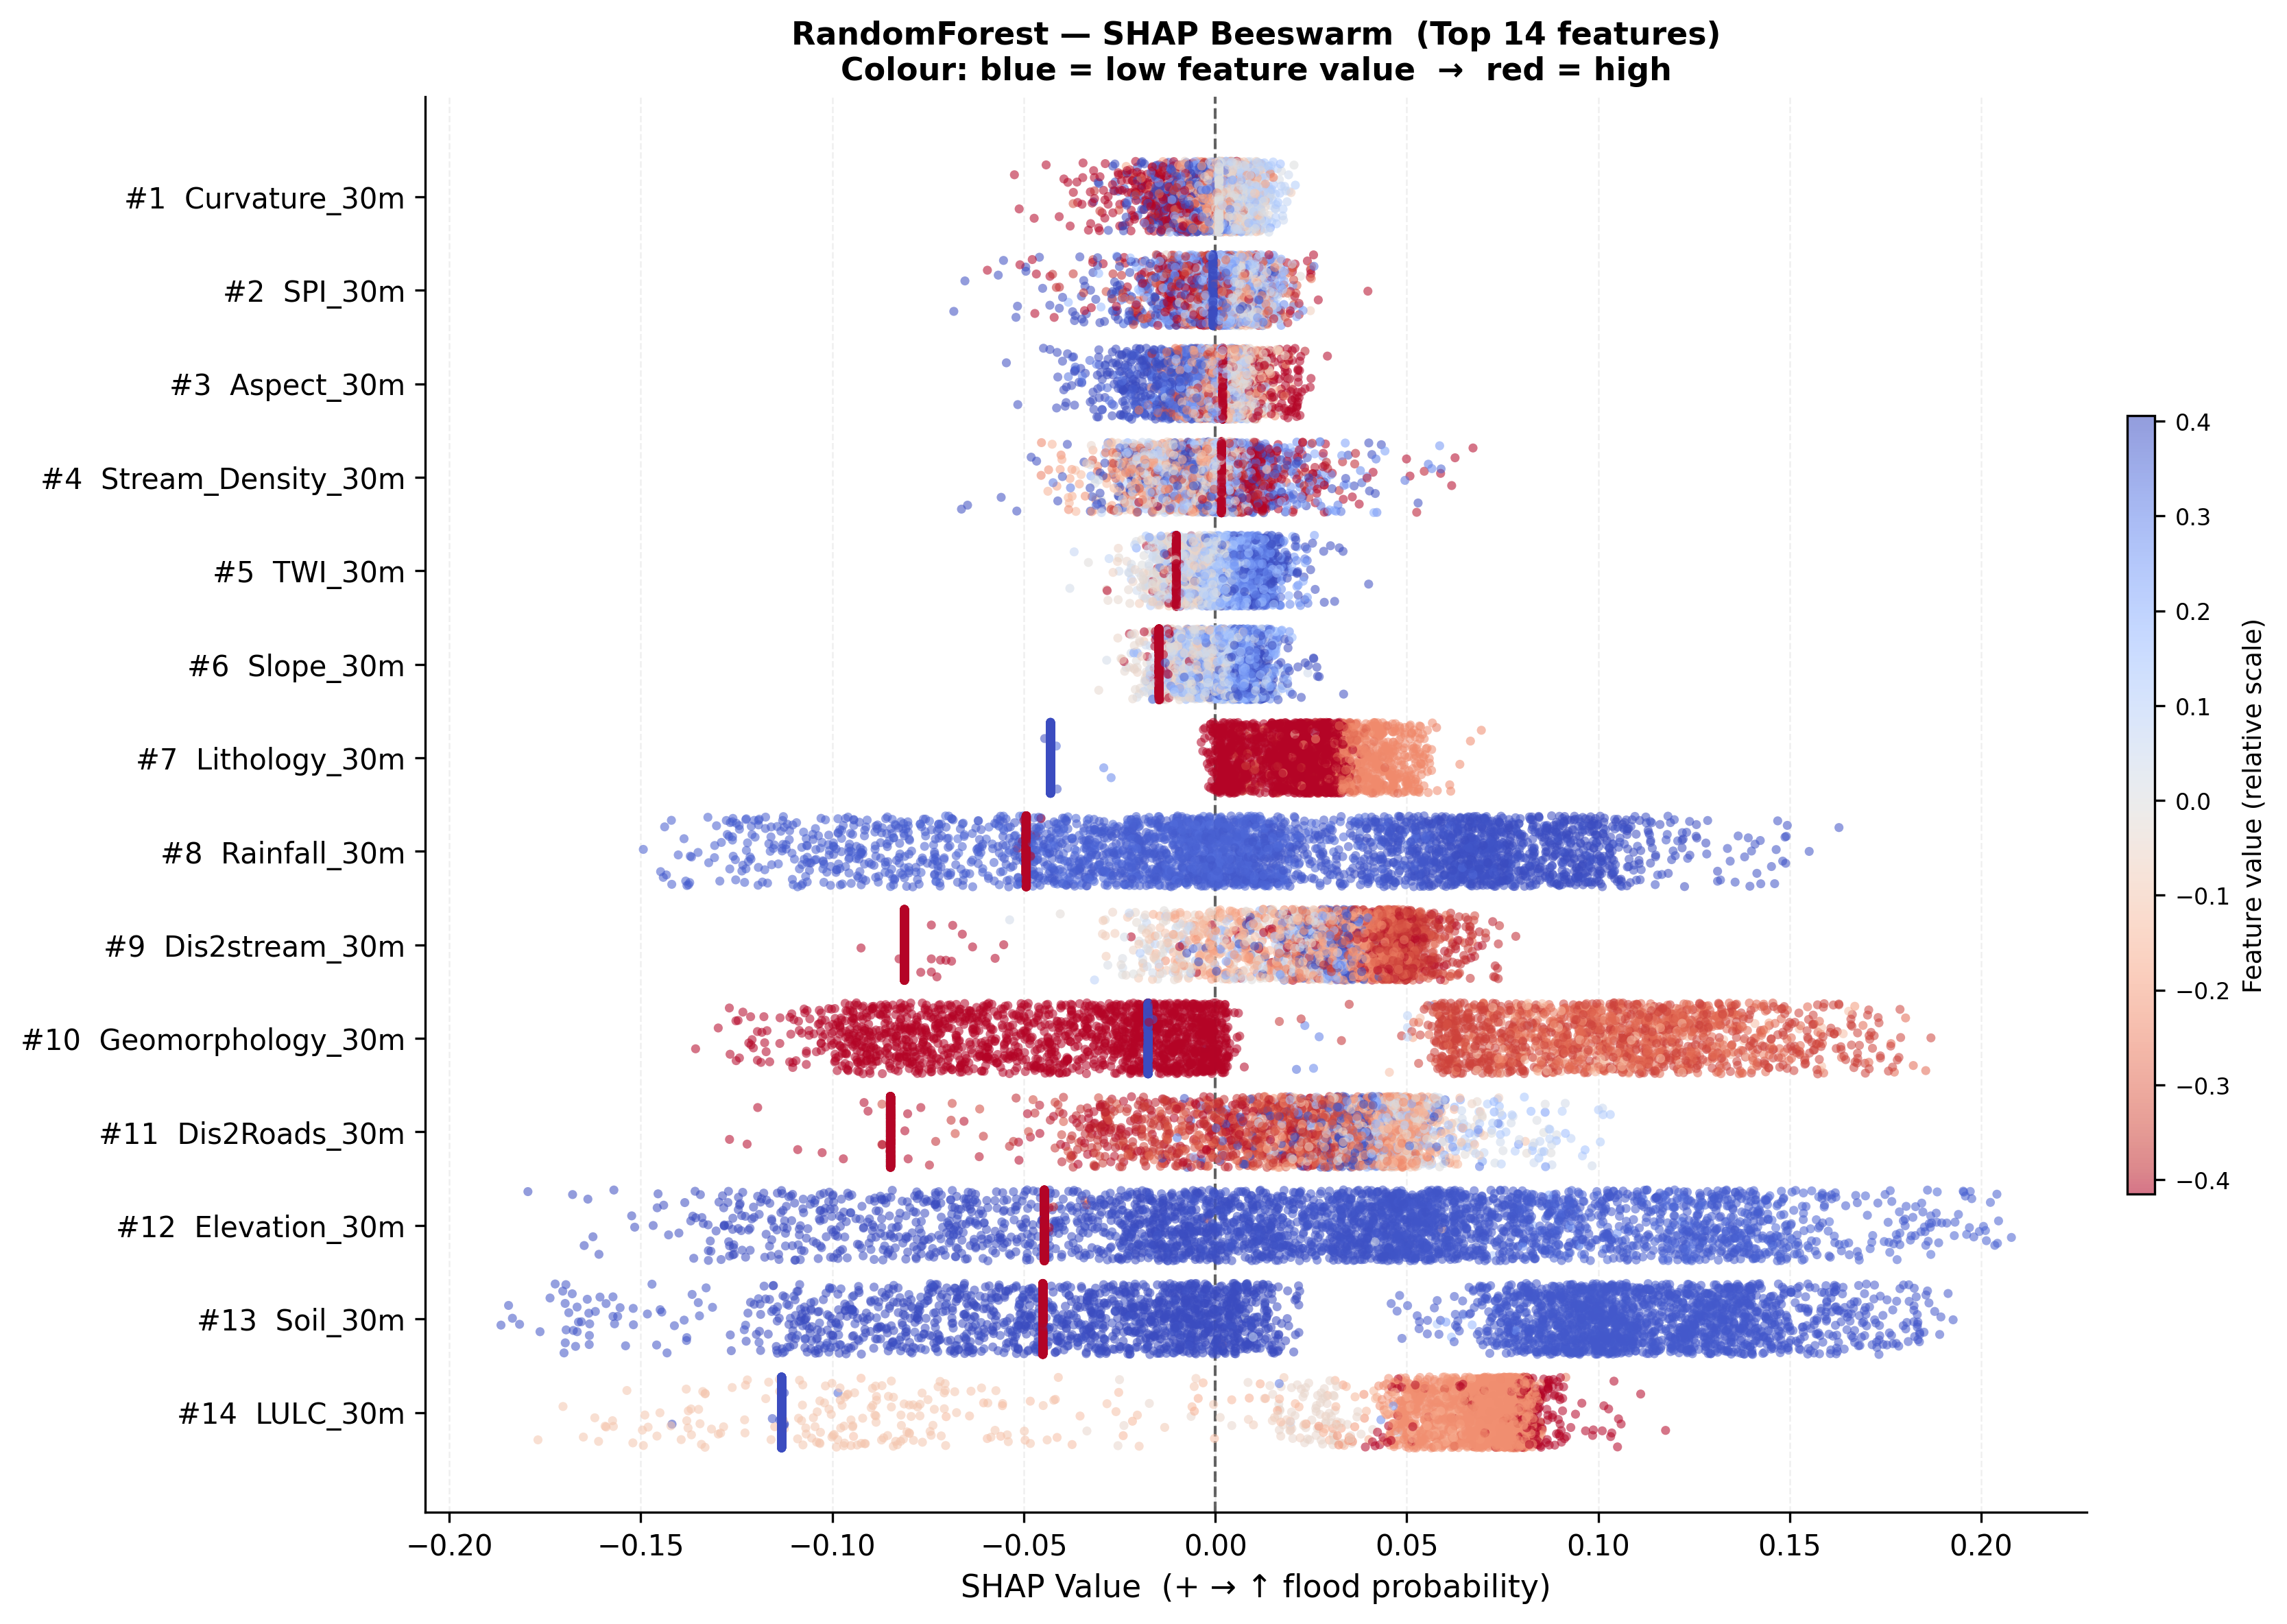
\includegraphics[width=\textwidth]{Figures/Fig_SHAP_Beeswarm_RandomForest.png}
  \caption{RandomForest SHAP beeswarm plot (top 13 features), computed via sklearn proxy RandomForest with 100 estimators. RF SHAP ranks confirm the tree-ensemble consensus: Geomorphology, Soil, and Rainfall in the top three.  The beeswarm distributions for RF are broader than XGBoost, reflecting higher variance in RF's bagging-based probability estimates.}
  \label{fig:shap_beeswarm_rf}
\end{figure}

\begin{figure}[H]
  \centering
  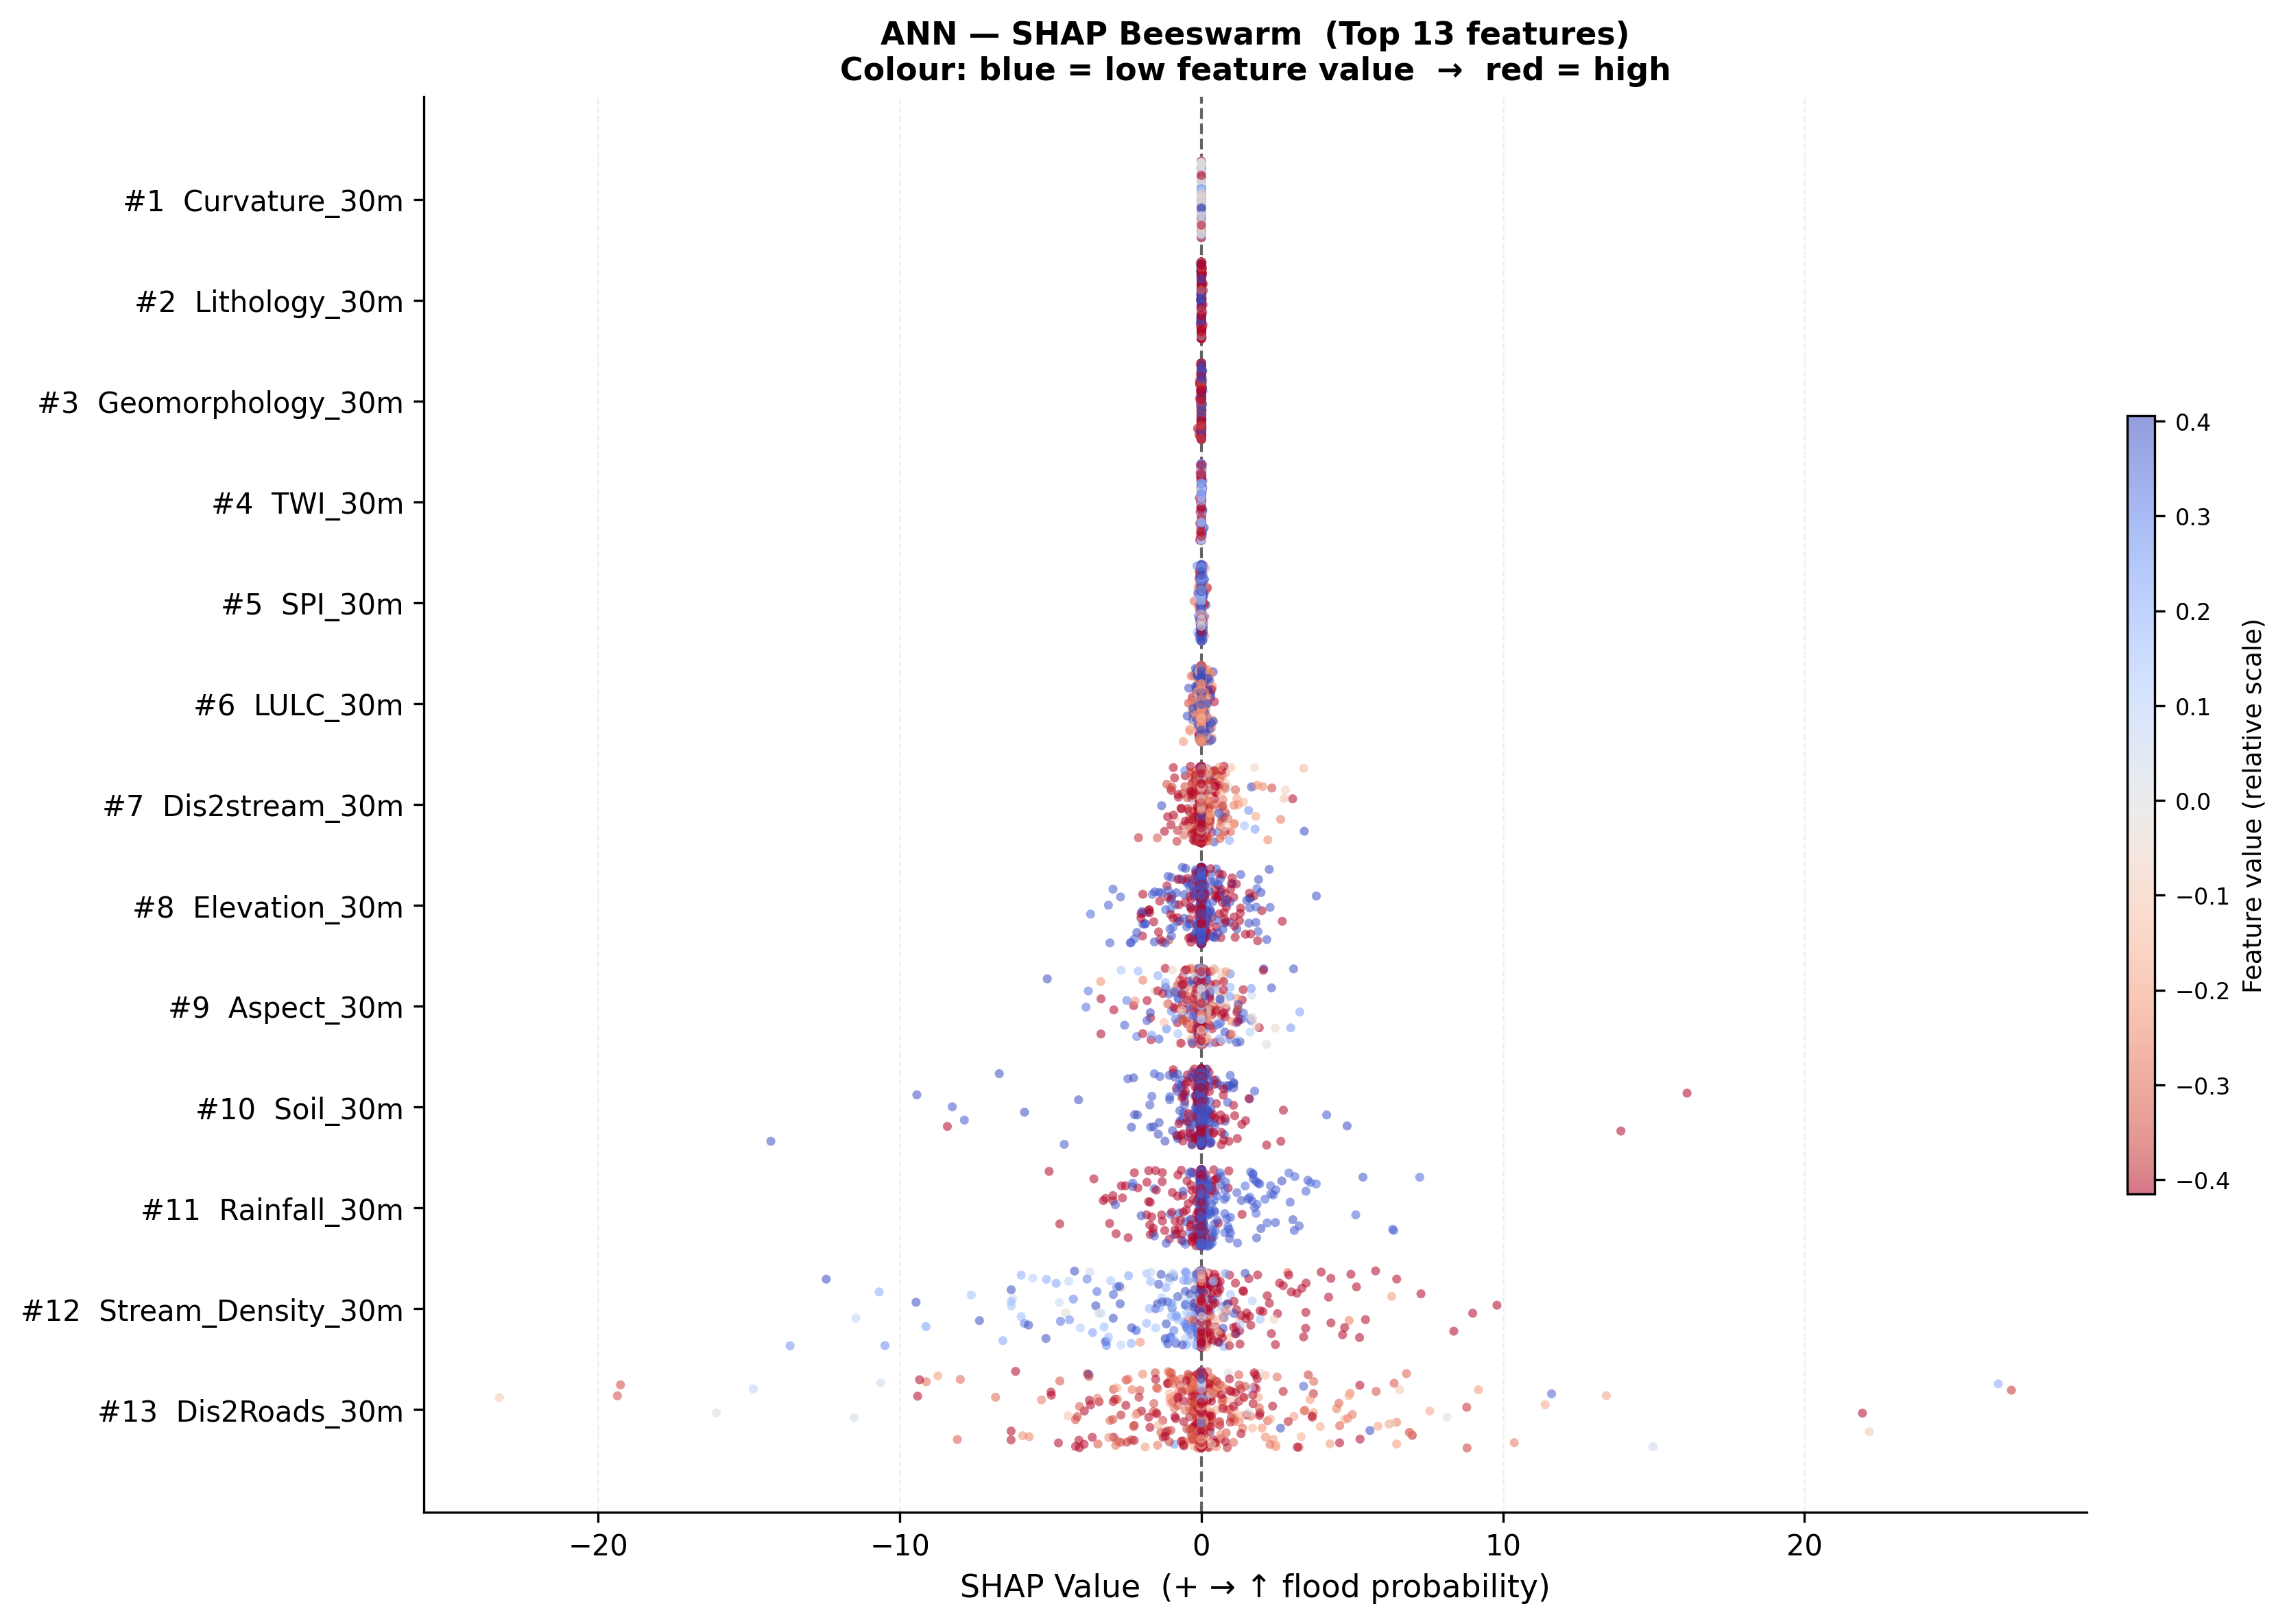
\includegraphics[width=\textwidth]{Figures/Fig_SHAP_Beeswarm_ANN.png}
  \caption{ANN SHAP beeswarm plot (top 12 features; Slope and TWI excluded).  GPU GradientExplainer (Integrated Gradients) on CUDA. ANN importance is more evenly distributed across features, consistent with the smooth neural activation surfaces.  Rainfall and Elevation rank highly, but the SHAP magnitude per feature is substantially lower than XGBoost, reflecting diffused probability contribution across many features.}
  \label{fig:shap_beeswarm_ann}
\end{figure}

\begin{figure}[H]
  \centering
  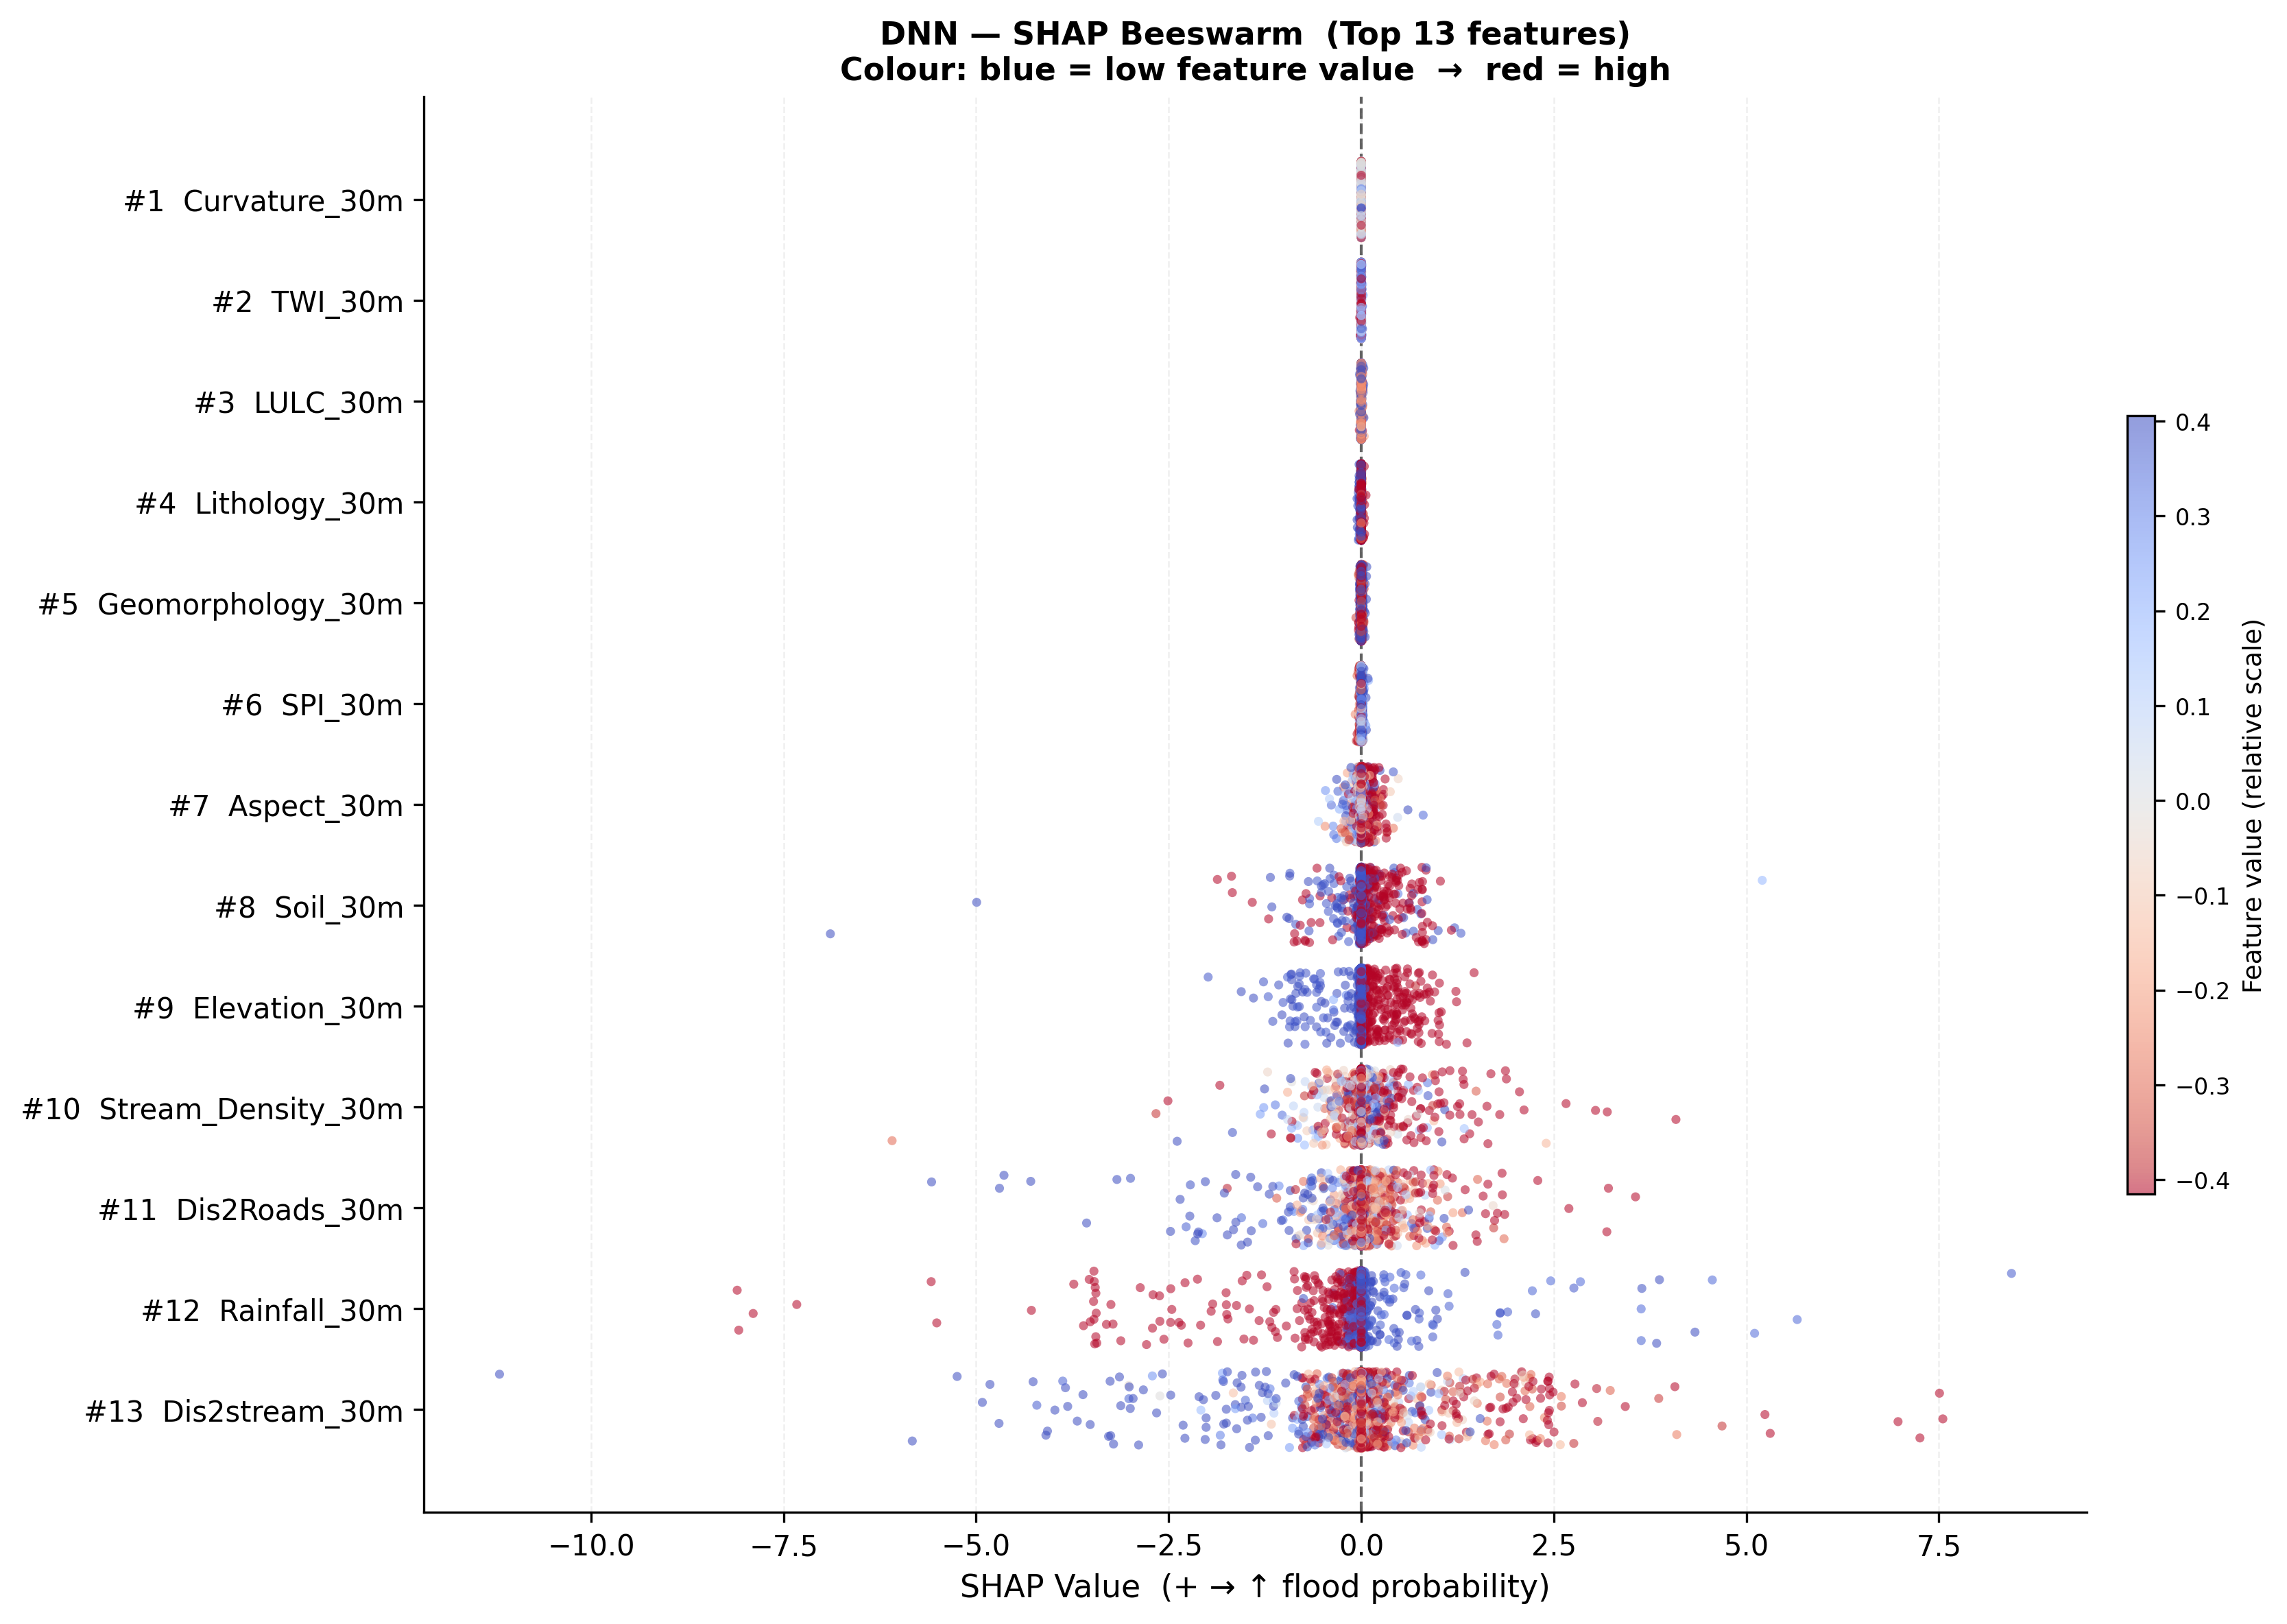
\includegraphics[width=\textwidth]{Figures/Fig_SHAP_Beeswarm_DNN.png}
  \caption{DNN SHAP beeswarm plot (top 12 features; Slope and TWI excluded).  GradientExplainer SHAP on CUDA. DNN importance profile is broadly similar to ANN, with slightly higher SHAP magnitudes for Geomorphology and Rainfall, reflecting the marginally deeper feature hierarchy of the three-layer architecture.  The absence of Slope and TWI from DNN inputs explains the lower importance of terrain indices relative to the tree-based model panels.}
  \label{fig:shap_beeswarm_dnn}
\end{figure}

\end{document}
